\documentclass[a4paper,12pt]{report}
\usepackage[utf8]{inputenc}
\usepackage[german]{babel}
\usepackage{lmodern}
\usepackage{amsmath}
\usepackage{amssymb}
\usepackage{amsthm}
\usepackage{geometry}
\usepackage{graphicx}
\usepackage{enumitem}
\usepackage{microtype}
\usepackage[hidelinks]{hyperref}
\usepackage{tikz}
\usepackage{circuitikz}

\usetikzlibrary{arrows.meta,positioning,calc}
\hypersetup{colorlinks=true,linkcolor=blue!60!black,urlcolor=blue!60!black,citecolor=blue!60!black}
\geometry{margin=2.5cm}
\setlist[itemize,1]{label=--}

\theoremstyle{definition}
\newtheorem{definition}{Definition}
\newtheorem{beispiel}{Beispiel}
\newtheorem{satz}{Satz}
\newtheorem{lemma}{Lemma}
\newtheorem{korollar}{Korollar}
\newtheorem{beobachtung}{Beobachtung}

\title{\textbf{Signaltheorie} \\ {\Large Das Wunder der e-Funktion}}
\author{Stephan Epp}
\date{23. Januar 2026}

\begin{document}
	
	\maketitle
	\tableofcontents
	\newpage
	
	\chapter{Einführung}
	
	\begin{definition}[Signal]
		Ein \textbf{Signal} ist eine Funktion, die Information über ein physikalisches Phänomen trägt. Mathematisch ist ein Signal eine Funktion $x(t)$, die einen Wert zu jedem Zeitpunkt $t$ hat.
		
		Signale können sein:
		\begin{itemize}
			\item[-] \textbf{Kontinuierlich}: Definiert für alle Zeiten $t \in \mathbb{R}$
			\item[-] \textbf{Diskret}: Definiert nur für bestimmte Zeitpunkte $t = nT$
			\item[-] \textbf{Deterministisch}: Vollständig vorhersehbar
			\item[-] \textbf{Stochastisch}: Zufällig oder mit Rauschen
		\end{itemize}
	\end{definition}
	
	\begin{beispiel}[Signale in der Natur]
		Beispiele für Signale in der Natur:
		\begin{itemize}
			\item[-] \textbf{Schallwellen}: Druckschwankungen in der Luft, die das Ohr wahrnimmt
			\item[-] \textbf{Lichtwellen}: Elektromagnetische Wellen, die das Auge sieht
			\item[-] \textbf{Elektrische Spannungen}: In Stromkreisen und elektronischen Geräten
			\item[-] \textbf{Seismische Wellen}: Vibrationen der Erde bei Erdbeben
			\item[-] \textbf{Biologische Signale}: Herzschlag, Gehirnaktivität (EEG), Muskelaktivität (EMG)
			\item[-] \textbf{Kommunikationssignale}: Radio, Fernsehen, Internet
		\end{itemize}
	\end{beispiel}
	
	\section{Warum Signaltheorie?}
	
	Signale sind überall. Aber warum brauchen wir eine Theorie, um sie zu verstehen? Warum nicht einfach die Signale messen und analysieren?
	
	Die Antwort ist: Weil Signale oft sehr komplex sind. Ein Musiksignal besteht aus Millionen von Schwingungen überlagert. Ein Kommunikationssignal ist mit Rauschen vermischt. Ein biologisches Signal ist von vielen Störquellen beeinflusst.
	
	Um diese komplexen Signale zu verstehen, zu analysieren und zu verarbeiten, brauchen wir \textbf{Werkzeuge}. Und diese Werkzeuge kommen aus der Signaltheorie.
	
	\begin{beobachtung}[Anwendungen]
		Praktische Anwendungen der Signaltheorie:
		\begin{itemize}
			\item[-] \textbf{Audio}: Kompression (MP3), Rauschunterdrückung, Equalizer
			\item[-] \textbf{Kommunikation}: Modulation, Filterung, Fehlerkorrektur
			\item[-] \textbf{Medizin}: EKG-Analyse, Bildverarbeitung, Diagnose
			\item[-] \textbf{Seismologie}: Erdbebenerkennung, Ressourcenerkundung
			\item[-] \textbf{Astronomie}: Signalverarbeitung von Teleskopen
			\item[-] \textbf{Finanzwesen}: Zeitreihenanalyse, Vorhersage
		\end{itemize}
	\end{beobachtung}
	
	Diese Arbeit stellt eine zentrale Frage: Gibt es ein universelles Signal, das alle anderen Signale beschreibt? Gibt es ein fundamentales Konzept, das die Struktur aller Signale erklärt? Die Antwort ist ja. Und dieses universelle Signal ist die \textbf{e-Funktion}.
	
	\begin{satz}[Zentrale Aussage]
		Die e-Funktion $e^{st}$ mit komplexem $s = \sigma + i\omega$ ist das universelle Signal. Sie ist:
		\begin{itemize}
			\item[-] Die natürliche Lösung aller linearen Differentialgleichungen
			\item[-] Die Eigenfunktion aller linearen zeitinvarianten Systeme
			\item[-] Die Basis aller Signalzerlegungen (Fourier, Laplace)
			\item[-] Das fundamentale Modell für Wachstum, Zerfall und Oszillation
		\end{itemize}
	\end{satz}
	
	Diese Arbeit beschreibt den Weg von der Praxis zur Theorie und zurück. Es wird sehen, wie die e-Funktion überall auftaucht -- in Stromkreisen, in biologischen Systemen, in Netzwerken, in der Signalverarbeitung.
	
	Wir beginnen in Kapitel 2 mit dem einfachsten nicht-trivialen dynamischen System: einem RL-Strom\-kreis (Spule und Widerstand). Wenn wir die Differentialgleichung für diesen Stromkreis lösen, erscheint die e-Funktion natürlich. Es wird sehen, wie die Zeitkonstante $\tau = L/R$ die Dynamik bestimmt, und wie die e-Funktion Aufbau und Abbau des Stroms beschreibt. \textbf{Lernziel}: Verstehen, dass die e-Funktion die natürliche Lösung von Differentialgleichungen ist.
	
	Dann wenden wir uns in Kapitel 3 einem biologischen Wunder zu: der Basilarmembran im Ohr. Diese Membran führt eine spektrale Zerlegung durch -- sie zerlegt Schallwellen in ihre Frequenzkomponenten. Dies ist eine biologische Fourier-Transformation, die die Natur Millionen Jahre vor der mathematischen Formulierung realisiert hat.
	
	Es wird sehen, wie die e-Funktion auch hier auftaucht -- in der exponentiellen Frequenzverteilung. Und es wird das Abtasttheorem aus der Physiologie motivieren: Warum können wir bis 20 kHz hören, aber nicht höher? \textbf{Lernziel}: Verstehen, dass biologische Systeme die gleichen mathematischen Prinzipien wie technische Systeme verwenden.
	
	In Kapitel 4 entwickeln wir dann die mathematische Fourier-Transformation. Dies ist ein mächtiges Werkzeug zur Zerlegung von Signalen in ihre Frequenzkomponenten. Es wird sehen, dass die e-Funktion $e^{i\omega t}$ die Basis dieser Zerlegung ist.
	
	Aber es wird auch die Grenzen der Fourier-Transformation erkennen: Sie ist nicht die beste Wahl für kontinuierliche Signale, weil sie keine Informationen über Wachstum und Zerfall enthält. \textbf{Lernziel}: Verstehen, dass die Fourier-Transformation eine Spezialfall einer allgemeineren Theorie ist.
	
	Dann untersuchen wir in Kapitel 5, wie Signale sich durch Netzwerke ausbreiten. Es wird sehen, dass die Adjazenzmatrix eines Netzwerks ein Signaloperator ist, und dass die Eigenwerte dieser Matrix das Langzeitverhalten bestimmen. Und wieder erscheint die e-Funktion -- diesmal als Matrixexponentialfunktion $e^{At}$. \textbf{Lernziel}: Verstehen, dass Netzwerk-Dynamik durch die e-Funktion beschrieben wird.
	
	In Kapitel 6 werden wir dann die theoretischen Konzepte durch umfangreiche Experimente validieren. Wir werden sehen, wie die e-Funktion in realen Systemen auftaucht: in RL- und RLC-Stromkreisen, in der Fourier-Analyse von Signalen, in Filterdesign, in der Signalausbreitung durch Netzwerke, und in der biologischen Fourier-Analyse der Basilarmembran. Diese Experimente werden zeigen, dass die Theorie nicht nur mathematisch elegant ist, sondern auch praktisch relevant. \textbf{Lernziel}: Verstehen, dass die theoretischen Konzepte in realen Systemen funktionieren.
	
	In Kapitel 7 synthetisieren wir alle Erkenntnisse. Es wird sehen, dass die e-Funktion $e^{st}$ mit komplexem $s = \sigma + i\omega$ alle Aspekte der Signaltheorie vereint:
	\begin{itemize}
		\item[-] Der Realteil $\sigma$ beschreibt Wachstum und Zerfall
		\item[-] Der Imaginärteil $\omega$ beschreibt Oszillation
		\item[-] Zusammen beschreiben sie alle Aspekte der Dynamik
	\end{itemize}
	
	Es wird auch die Laplace-Transformation kennenlernen -- die natürliche Verallgemeinerung der Fourier-Transformation. \textbf{Lernziel}: Verstehen, dass die e-Funktion das universelle Signal ist.
	
	Dann sehen wir in Kapitel 8, wie die theoretischen Konzepte in der Praxis angewendet werden. Wir entwerfen Filter, modulieren Signale, und implementieren digitale Signalverarbeitung. Es wird sehen, dass die Theorie direkt zu praktischen Werkzeugen führt. \textbf{Lernziel}: Verstehen, dass Theorie und Praxis zusammenhängen.
	
	In Kapitel 9 reflektieren wir über die Bedeutung der e-Funktion. Es wird sehen, dass sie nicht nur ein mathematisches Werkzeug ist, sondern ein Fenster in die fundamentale Struktur der Natur. \textbf{Lernziel}: Verstehen, dass die e-Funktion ein Urmodell der Natur ist.
	
	Abschließend erkunden wir in Kapitel 10 eine fundamentale Asymmetrie: Ableitungen sind viel leichter durchzuführen als Integrale. Dies ist nicht nur eine mathematische Beobachtung, sondern ein tiefes Prinzip, das die gesamte moderne Signalverarbeitung prägt. Es wird sehen, warum dieser Asymmetrie zu einem Paradigmenwechsel geführt hat: weg von Laplace- und Fourier-Transformationen (Bildbereich) hin zu direkter Zeitbereichsanalyse mit Ableitungen und Differenzengleichungen.
	
	Es wird auch verstehen, warum nach der Digitalisierung eines Signals die klassischen Transformationen nicht mehr die erste Wahl sind. Stattdessen arbeitet die moderne Signalverarbeitung direkt im Zeitbereich mit adaptiven Algorithmen, die sich an sich ändernde Signale anpassen. Die Basilarmembran zeigt, dass die Natur schon lange diesen Weg geht: Sie arbeitet direkt mit kontinuierlichen Signalen, führt eine räumliche Abtastung durch, und konvertiert dann in neuronale Impulse.
	
	\textbf{Lernziel}: Verstehen, dass die Asymmetrie zwischen Ableitungen und Integralen ein fundamentales Prinzip der modernen Signalverarbeitung ist, und dass der Zeitbereich die natürliche Domäne für praktische Anwendungen ist.
	
	
	\section{Die Zerlegung in gerade und ungerade Komponenten}
	
	Ein wichtiges Konzept, das sich durch diese Arbeit zieht, ist die \textbf{Zerlegung in gerade und ungerade Komponenten}. Dies wurde in der früheren Arbeit über die Exponentialreihe eingeführt:
	
	\begin{align}
		e^x = E(x) + U(x) = \cosh(x) + \sinh(x)
	\end{align}
	
	wobei $E(x) = \cosh(x)$ die gerade Komponente und $U(x) = \sinh(x)$ die ungerade Komponente ist.
	
	Diese Zerlegung manifestiert sich überall in der Signaltheorie:
	\begin{itemize}
		\item[-] In der Fourier-Transformation: $e^{i\omega t} = \cos(\omega t) + i\sin(\omega t)$
		\item[-] In der komplexen e-Funktion: $e^{st} = e^{\sigma t}[\cos(\omega t) + i\sin(\omega t)]$
		\item[-] In der Fourier-Reihe: Cosinus-Komponenten (gerade) und Sinus-Komponenten (ungerade)
	\end{itemize}
	
	Diese fundamentale Dualität ist nicht zufällig. Sie spiegelt eine tiefe Struktur der Natur wider.
	
	\section{Zentrale Aussage}
	
	Die zentrale Aussage dieser Arbeit ist einfach: Die e-Funktion ist nicht nur ein mathematisches Werkzeug. Sie ist das Urmodell aller Signale und Dynamik. Sie zeigt uns, dass Komplexität aus Einfachheit entsteht, dass Vielfalt aus Einheit kommt, und dass die Natur nach eleganten Prinzipien funktioniert.
	
	\chapter{RL-Stromkreis: Erste Begegnung mit e-Funktion}
	
	\section{Das einfachste dynamische System}
	
	Betrachten wir den einfachsten nicht-trivialen elektrischen Stromkreis: eine Spule (Induktivität $L$) in Reihe mit einem Widerstand $R$, gespeist von einer Spannungsquelle $U(t)$.
	
	\begin{figure}[htbp]
		\centering
		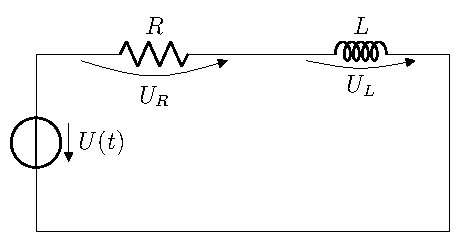
\includegraphics[width=0.7\textwidth]{cir-rl-circuit.pdf}
		\caption{RL-Stromkreis als Reihenschaltung mit Widerstand $R$ und Induktivität $L$}
		\label{fig:cir-rl-circuit}
	\end{figure}
	
	\begin{definition}[Kirchhoffsche Maschenregel]
		Die Summe aller Spannungen entlang einer geschlossenen Masche ist Null:
		\begin{align}
			U(t) - U_R(t) - U_L(t) = 0
		\end{align}
		
		Mit dem \textbf{Ohmschen Gesetz} $U_R = R \cdot i$ und dem \textbf{Induktionsgesetz} $U_L = L \frac{di}{dt}$ folgt:
		\begin{align}
			U(t) = R \cdot i(t) + L \frac{di(t)}{dt}
		\end{align}
	\end{definition}
	
	Dies ist eine lineare Differentialgleichung erster Ordnung. Die Struktur dieser Gleichung ist fundamental: Sie verbindet den aktuellen Zustand $i(t)$ mit seiner Änderungsrate $\frac{di}{dt}$.
	
	\section{Lösung für Gleichspannung}
	
	Für den Fall, dass die Spannungsquelle zum Zeitpunkt $t = 0$ eingeschaltet wird, lautet die Lösung:
	
	\begin{satz}[Lösung der RL-Differentialgleichung]
		Für Anfangsbedingung $i(0) = 0$ und konstante Spannung $U(t) = U_0$ für $t > 0$ ist die Lösung:
		\begin{align}
			i(t) = \frac{U_0}{R} \left(1 - e^{-\frac{R}{L}t}\right) = \frac{U_0}{R} \left(1 - e^{-\frac{t}{\tau}}\right)
		\end{align}
		
		wobei $\tau = \frac{L}{R}$ die \textbf{Zeitkonstante} des Systems ist.
	\end{satz}
	
	\begin{proof}
		Die Differentialgleichung lautet für $t > 0$:
		\begin{align}
			L \frac{di}{dt} + R i = U_0
		\end{align}
		
		\textbf{Schritt 1: Homogene Lösung}
		
		Die homogene Gleichung $L \frac{di}{dt} + R i = 0$ kann umgeschrieben werden als:
		\begin{align}
			\frac{di}{dt} = -\frac{R}{L} i
		\end{align}
		
		Dies ist die Standardform einer Exponentialgleichung. Der Ansatz $i_h(t) = C e^{\lambda t}$ führt zu:
		\begin{align}
			\lambda C e^{\lambda t} = -\frac{R}{L} C e^{\lambda t} \quad \Rightarrow \quad \lambda = -\frac{R}{L}
		\end{align}
		
		Also: $i_h(t) = C e^{-\frac{R}{L}t}$.
		
		\textbf{Schritt 2: Partikuläre Lösung}
		
		Für die inhomogene Gleichung suchen wir eine konstante Lösung: $i_p(t) = i_{\infty}$.
		Einsetzen ergibt:
		\begin{align}
			L \cdot 0 + R i_{\infty} = U_0 \quad \Rightarrow \quad i_{\infty} = \frac{U_0}{R}
		\end{align}
		
		Dies ist der \textbf{stationäre Strom} -- der Strom, der sich für $t \to \infty$ einstellt.
		
		\textbf{Schritt 3: Allgemeine Lösung}
		
		Die allgemeine Lösung ist die Summe:
		\begin{align}
			i(t) = i_h(t) + i_p(t) = C e^{-\frac{R}{L}t} + \frac{U_0}{R}
		\end{align}
		
		\textbf{Schritt 4: Anfangsbedingung}
		
		Aus $i(0) = 0$ folgt:
		\begin{align}
			0 = C e^0 + \frac{U_0}{R} = C + \frac{U_0}{R} \quad \Rightarrow \quad C = -\frac{U_0}{R}
		\end{align}
		
		Somit:
		\begin{align}
			i(t) = -\frac{U_0}{R} e^{-\frac{R}{L}t} + \frac{U_0}{R} = \frac{U_0}{R} \left(1 - e^{-\frac{R}{L}t}\right)
		\end{align}
	\end{proof}
	
	\section{Die Zeitkonstante als fundamentales Maß}
	
	\begin{definition}[Zeitkonstante]
		Die Zeitkonstante $\tau = \frac{L}{R}$ ist die charakteristische Zeit des Systems. Sie hat folgende Bedeutungen:
		
		\begin{enumerate}
			\item[-] Nach Zeit $t = \tau$ hat der Strom den Wert:
			\begin{align}
				i(\tau) = \frac{U_0}{R}(1 - e^{-1}) = \frac{U_0}{R} \cdot 0.632... \approx 63.2\% \text{ des Endwerts}
			\end{align}
			
			\item[-] Nach Zeit $t = 5\tau$ (oft als "praktisch unendlich" betrachtet):
			\begin{align}
				i(5\tau) = \frac{U_0}{R}(1 - e^{-5}) = \frac{U_0}{R} \cdot 0.993... \approx 99.3\% \text{ des Endwerts}
			\end{align}
			
			\item[-] Die Zeitkonstante ist das Verhältnis von Induktivität zu Widerstand:
			\begin{align}
				\tau = \frac{L}{R} = \frac{\text{Energiespeicher}}{\text{Energieverlust pro Zeit}}
			\end{align}
		\end{enumerate}
	\end{definition}
	
	\begin{beobachtung}[Asymmetrie zwischen Aufbau und Abbau]
		Die e-Funktion beschreibt sowohl den Aufbau ($1 - e^{-t/\tau}$) als auch den Abbau ($e^{-t/\tau}$) des Stroms. Diese Asymmetrie manifestiert sich in der Zerlegung:
		\begin{align}
			i(t) = \underbrace{\frac{U_0}{R}}_{\text{Stationär}} - \underbrace{\frac{U_0}{R} e^{-t/\tau}}_{\text{Transient}}
		\end{align}
		
		Der \textbf{stationäre Anteil} ist zeitunabhängig (eine Konstante, also eine "gerade Funktion" der Ordnung 0), der \textbf{transiente Anteil} ist zeitabhängig und klingt exponentiell ab.
		
		Dies ist eine erste Manifestation der Zerlegung in gerade und ungerade Komponenten, die wir aus der Exponentialreihe kennen!
	\end{beobachtung}
	
	\section{Energiebetrachtung}
	
	Die Energie in der Spule ist gegeben durch:
	\begin{align}
		W_L(t) = \frac{1}{2} L i(t)^2 = \frac{1}{2} L \left(\frac{U_0}{R}\right)^2 \left(1 - e^{-t/\tau}\right)^2
	\end{align}
	
	Die im Widerstand dissipierte Leistung ist:
	\begin{align}
		P_R(t) = R i(t)^2 = R \left(\frac{U_0}{R}\right)^2 \left(1 - e^{-t/\tau}\right)^2 = \frac{U_0^2}{R} \left(1 - e^{-t/\tau}\right)^2
	\end{align}
	
	Die gesamte dissipierte Energie bis zur Zeit $t$ ist:
	\begin{align}
		E_R(t) = \int_0^t P_R(\tau) d\tau = \int_0^t \frac{U_0^2}{R} \left(1 - e^{-\tau/\tau_0}\right)^2 d\tau
	\end{align}
	
	\begin{satz}[Energiebilanz]
		Die von der Quelle gelieferte Energie wird teils in der Spule gespeichert, teils im Widerstand dissipiert:
		\begin{align}
			W_{\text{Quelle}}(t) = W_L(t) + E_R(t)
		\end{align}
		
		Für $t \to \infty$:
		\begin{itemize}
			\item[-] Die Spule speichert: $W_L(\infty) = \frac{1}{2} L \left(\frac{U_0}{R}\right)^2$
			\item[-] Die Leistungsdissipation konvergiert gegen: $P_R(\infty) = \frac{U_0^2}{R}$
			\item[-] Die transiente Energie wurde vollständig im Widerstand dissipiert
		\end{itemize}
	\end{satz}
	
	\section{Die e-Funktion als natürliche Antwort}
	
	\begin{lemma}[Eigenfunktion der Differentiation]
		Die e-Funktion ist Eigenfunktion des Differentialoperators:
		\begin{align}
			\frac{d}{dt} e^{st} = s \cdot e^{st}
		\end{align}
		
		Dies erklärt, warum $e^{st}$ die natürliche Lösung linearer Differentialgleichungen mit konstanten Koeffizienten ist.
	\end{lemma}
	
	\begin{proof}
		Durch direkte Berechnung:
		\begin{align}
			\frac{d}{dt} e^{st} = \frac{d}{dt} \sum_{n=0}^{\infty} \frac{(st)^n}{n!} = \sum_{n=1}^{\infty} \frac{s \cdot n \cdot (st)^{n-1}}{n!} = s \sum_{n=1}^{\infty} \frac{(st)^{n-1}}{(n-1)!} = s e^{st}
		\end{align}
	\end{proof}
	
	Für die RL-Schaltung bedeutet dies:
	\begin{align}
		L \frac{di}{dt} + R i = 0 \quad \Rightarrow \quad L s + R = 0 \quad \Rightarrow \quad s = -\frac{R}{L}
	\end{align}
	
	Der Eigenwert $s = -R/L$ ist negativ, daher klingt die Lösung ab. Dies entspricht der dissipativen Natur des Widerstands -- Energie wird in Wärme umgewandelt.
	
	\section{Verallgemeinerung: Der RLC-Reihenschwingkreis}
	
	Für einen RLC-Reihenschwingkreis kommt zum Widerstand $R$ und zur Induktivität $L$ noch ein Kondensator (Kapazität $C$) hinzu.
	
	\begin{figure}[htbp]
		\centering
		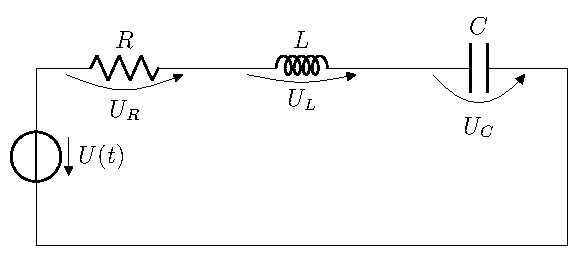
\includegraphics[width=0.7\textwidth]{cir-rlc-circuit.pdf}
		\caption{RLC-Stromkreis mit Widerstand $R$, Induktivität $L$ und Kondensator $C$}
		\label{fig:cir-rlc-circuit}
	\end{figure}
	
	Die Spannung am Kondensator ist:
	\begin{align}
		U_C(t) = \frac{1}{C} \int_0^t i(\tau) d\tau
	\end{align}
	
	Die Differentialgleichung wird:
	\begin{align}
		L \frac{di}{dt} + R i + \frac{1}{C} \int i(\tau) d\tau = U(t)
	\end{align}
	
	Durch Differentiation nach $t$:
	\begin{align}
		L \frac{d^2i}{dt^2} + R \frac{di}{dt} + \frac{1}{C} i = \frac{dU}{dt}
	\end{align}
	
	Für $U(t) = U_0$ ist $\frac{dU}{dt} = U_0 \text{ } \delta(t)$ (Dirac-Impuls bei $t=0$, dann Null).
	
	Die charakteristische Gleichung ist:
	\begin{align}
		L s^2 + R s + \frac{1}{C} = 0 \quad \Rightarrow \quad s_{1,2} = -\frac{R}{2L} \pm \sqrt{\left(\frac{R}{2L}\right)^2 - \frac{1}{LC}}
	\end{align}
	
	\begin{definition}[Dämpfungstypen]
		Abhängig von der Diskriminante $\Delta = \left(\frac{R}{2L}\right)^2 - \frac{1}{LC}$ unterscheidet man:
		
		\begin{itemize}
			\item[-] \textbf{Überdämpft} ($\Delta > 0$, d.h. $R^2 > 4L/C$): 
			\begin{itemize}
				\item[-] Zwei reelle negative Eigenwerte $s_1, s_2 < 0$
				\item[-] Exponentielles Abklingen ohne Oszillation
				\item[-] Lösung: $i(t) = A_1 e^{s_1 t} + A_2 e^{s_2 t}$
			\end{itemize}
			
			\item[-] \textbf{Kritisch gedämpft} ($\Delta = 0$, d.h. $R^2 = 4L/C$): 
			\begin{itemize}
				\item[-] Doppelter reeller Eigenwert $s = -\frac{R}{2L}$
				\item[-] Schnellstmögliches Abklingen ohne Überschwingen
				\item[-] Lösung: $i(t) = (A + Bt) e^{st}$
			\end{itemize}
			
			\item[-] \textbf{Unterdämpft} ($\Delta < 0$, d.h. $R^2 < 4L/C$): 
			\begin{itemize}
				\item[-] Komplex konjugierte Eigenwerte
				\item[-] Gedämpfte Oszillation
			\end{itemize}
		\end{itemize}
	\end{definition}
	
	Für den unterdämpften Fall schreiben wir die Eigenwerte als:
	\begin{align}
		s_{1,2} = -\underbrace{\frac{R}{2L}}_{\sigma} \pm i\underbrace{\sqrt{\frac{1}{LC} - \left(\frac{R}{2L}\right)^2}}_{\omega_d}
	\end{align}
	
	wobei:
	\begin{itemize}
		\item[-] $\sigma = \frac{R}{2L}$ die \textbf{Dämpfungskonstante} ist
		\item[-] $\omega_d = \sqrt{\frac{1}{LC} - \left(\frac{R}{2L}\right)^2}$ die \textbf{gedämpfte Kreisfrequenz} ist
		\item[-] $\omega_0 = \frac{1}{\sqrt{LC}}$ die \textbf{ungedämpfte Eigenfrequenz} ist
	\end{itemize}
	
	Die Lösung für die homogene Gleichung ist:
	\begin{align}
		i(t) = e^{-\sigma t} \left(A \cos(\omega_d t) + B \sin(\omega_d t)\right) = C e^{-\sigma t} \cos(\omega_d t + \phi)
	\end{align}
	
	wobei $C$ und $\phi$ durch die Anfangsbedingungen bestimmt werden.
	
	\begin{beobachtung}[Zerlegung in gerade und ungerade Komponenten]
		Die Lösung lässt sich schreiben als:
		\begin{align}
			i(t) = \text{Re}\left(C e^{s_1 t}\right) = \text{Re}\left(C e^{-\sigma t} e^{i\omega_d t}\right)
		\end{align}
		
		Mit der Euler-Formel $e^{i\omega t} = \cos(\omega t) + i\sin(\omega t)$ ergibt sich:
		\begin{align}
			i(t) = e^{-\sigma t} \underbrace{\left(C_1 \cos(\omega_d t)\right)}_{\text{Gerade Funktion von } t} + e^{-\sigma t} \underbrace{\left(C_2 \sin(\omega_d t)\right)}_{\text{Ungerade Funktion von } t}
		\end{align}
		
		Die Dämpfung $e^{-\sigma t}$ moduliert beide Komponenten gleichermaßen -- sie ist die \textbf{Einhül\-lende} der Oszillation.
		
		\textbf{Fundamentale Beobachtung}: Die e-Funktion $e^{st}$ mit komplexem $s = \sigma + i\omega$ vereint:
		\begin{itemize}
			\item[-] Den exponentiellen Zerfall (gerade Komponente bezüglich des Realteils)
			\item[-] Die harmonische Oszillation (ungerade und gerade trigonometrische Funktionen)
		\end{itemize}
		
		Dies ist genau die Zerlegung $e^{ix} = \cos(x) + i\sin(x)$ aus der Exponentialreihe!
	\end{beobachtung}
	
	\chapter{Das Wunder der Membran}
	
	\section{Basilarmembran: Biologischer Fourier-Analysator}
	
	Die Basilarmembran im Ohr vollbringt ein Wunder der Natur: Sie transformiert kontinuierliche Schallwellen in diskrete neuronale Impulse. Verschiedene Frequenzen erzeugen maximale Auslenkung an verschiedenen Orten -- eine \textbf{biologische Fourier-Transformation}. Dies ist nicht nur eine Metapher, sondern eine echte mathematische Zerlegung, die die Natur viele Jahre vor der Erfindung der Fourier-Analyse realisiert hat.
	
	\subsection{Anatomie und Physiologie}
	
	Die Cochlea (Schnecke) ist ein spiralförmiger Kanal im Innenohr, gefüllt mit Flüssigkeit (Perilymphe). Die Basilarmembran ist eine elastische Struktur, die den Kanal in zwei Teile teilt. Auf der Basilarmembran sitzen etwa 16.000 Haarzellen (bei Menschen), die als Mechanorezeptoren fungieren.
	
	\begin{definition}[Basilarmembran-Eigenschaften]
		Die Basilarmembran hat folgende charakteristische Eigenschaften:
		\begin{itemize}
			\item[-] \textbf{Länge}: Etwa 35 mm beim Menschen
			\item[-] \textbf{Breite}: Variiert von etwa 0,1 mm am ovalen Fenster (basal) bis 0,5 mm an der Spitze (apikal)
			\item[-] \textbf{Steifigkeit}: Nimmt exponentiell vom basalen zum apikalen Ende ab
			\item[-] \textbf{Masse}: Nimmt vom basalen zum apikalen Ende zu
		\end{itemize}
		
		Diese Variation ist \textbf{nicht zufällig}, sondern optimal für die Frequenzzerlegung!
	\end{definition}
	
	\subsection{Die Wellenausbreitung}
	
	Wenn Schallwellen das ovale Fenster (Eingang zur Cochlea) erreichen, erzeugen sie Druckwellen in der Perilymphe. Diese Wellen breiten sich entlang der Basilarmembran aus. Die Membran verhält sich wie ein \textbf{dispersives Medium}: Verschiedene Frequenzen breiten sich mit unterschiedlichen Geschwindigkeiten aus und erreichen ihre maximale Auslenkung an verschiedenen Orten.
	
	\begin{satz}[Tonotopische Organisation]
		Die charakteristische Frequenz an Ort $x$ (gemessen vom basalen Ende) ist:
		\begin{align}
			f(x) = f_0 \cdot e^{-\alpha x}
		\end{align}
		
		mit typischen Werten:
		\begin{itemize}
			\item[-] $f_0 \approx 20$ kHz (am basalen Ende, hohe Frequenzen)
			\item[-] $\alpha \approx 0.06$ mm$^{-1}$ (Abklingkonstante)
			\item[-] Am apikalen Ende: $f \approx 20$ Hz (tiefe Frequenzen)
		\end{itemize}
		
		Diese \textbf{logarithmische Frequenzskala} ist optimal für die menschliche Wahrnehmung, da wir Frequenzen logarithmisch wahrnehmen (eine Oktave ist eine Verdopplung der Frequenz).
	\end{satz}
	
	\begin{proof}[Heuristische Begründung]
		Die Steifigkeit der Membran nimmt exponentiell ab:
		\begin{align}
			k(x) = k_0 e^{-\beta x}
		\end{align}
		
		Die Masse pro Längeneinheit nimmt exponentiell zu:
		\begin{align}
			m(x) = m_0 e^{\gamma x}
		\end{align}
		
		Die Eigenfrequenz eines Membransegments ist:
		\begin{align}
			f(x) \propto \sqrt{\frac{k(x)}{m(x)}} = \sqrt{\frac{k_0 e^{-\beta x}}{m_0 e^{\gamma x}}} = \sqrt{\frac{k_0}{m_0}} e^{-(\beta + \gamma)x/2}
		\end{align}
		
		Dies ist genau die beobachtete exponentielle Abhängigkeit!
	\end{proof}
	
	\section{Die Haarzellen und neuronale Kodierung}
	
	\subsection{Mechanotransduktion}
	
	Die Haarzellen sind spezialisierte Sensoren, die mechanische Bewegung in elektrische Signale umwandeln. Jede Haarzelle hat etwa 100-150 Stereozilien (haarähnliche Strukturen), die in einer Reihe angeordnet sind.
	
	\begin{definition}[Mechanotransduktion-Kaskade]
		\begin{enumerate}
			\item[-] \textbf{Mechanische Auslenkung}: Die Basilarmembran bewegt sich um Nanometer
			\item[-] \textbf{Stereozilien-Bewegung}: Die Stereozilien biegen sich und öffnen Ionenkanäle
			\item[-] \textbf{Ioneneinstrom}: Kalium-Ionen (K$^+$) strömen in die Haarzelle
			\item[-] \textbf{Depolarisation}: Das Membranpotential wird weniger negativ
			\item[-] \textbf{Kalzium-Einstrom}: Spannungsgesteuerte Kalzium-Kanäle öffnen sich
			\item[-] \textbf{Neurotransmitter-Freisetzung}: Glutamat wird an den Synapsen freigesetzt
			\item[-] \textbf{Neuronale Aktivierung}: Der Hörnerv feuert Aktionspotenziale
		\end{enumerate}
	\end{definition}
	
	\subsection{Frequenzselektivität}
	
	Jede Haarzelle ist am stärksten auf ihre charakteristische Frequenz $f_c$ empfindlich. Dies wird durch mehrere Mechanismen erreicht:
	
	\begin{itemize}
		\item[-] \textbf{Mechanische Resonanz}: Die Basilarmembran resoniert bei ihrer Eigenfrequenz
		\item[-] \textbf{Aktive Verstärkung}: Äußere Haarzellen kontrahieren und verstärken die Bewegung
		\item[-] \textbf{Neuronale Filterung}: Der Hörnerv selbst hat Frequenzselektivität
	\end{itemize}
	
	\begin{satz}[Frequenzselektivität der Haarzellen]
		Die Antwort einer Haarzelle auf ein Sinussignal $x(t) = A \sin(2\pi f t)$ ist maximal bei der charakteristischen Frequenz $f_c$ und fällt ab für $f \neq f_c$. Die Bandbreite ist typischerweise:
		\begin{align}
			\Delta f \approx 0.1 \cdot f_c
		\end{align}
		
		Dies ist die \textbf{Güte} des Filters: $Q = f_c / \Delta f \approx 10$.
	\end{satz}
	
	\section{Das Abtasttheorem und die Grenzen des Hörens}
	
	\subsection{Das Nyquist-Shannon-Abtasttheorem}
	
	\begin{satz}[Nyquist-Shannon-Abtasttheorem]
		Ein kontinuierliches Signal $x(t)$ mit maximaler Frequenz $f_{\max}$ (bandbegrenzt) kann perfekt rekonstruiert werden aus Abtastwerten $x(nT)$, falls die Abtastfrequenz:
		\begin{align}
			f_s = \frac{1}{T} > 2 f_{\max}
		\end{align}
		
		Die Rekonstruktion erfolgt durch:
		\begin{align}
			x(t) = \sum_{n=-\infty}^{\infty} x(nT) \cdot \text{sinc}\left(\frac{t - nT}{T}\right)
		\end{align}
		
		wobei $\text{sinc}(u) = \frac{\sin(\pi u)}{\pi u}$ die Sinc-Funktion ist.
	\end{satz}
	
	\begin{proof}[Intuitive Erklärung]
		Die Sinc-Funktion hat die Eigenschaft:
		\begin{align}
			\text{sinc}(n) = \begin{cases} 1 & n = 0 \\ 0 & n \in \mathbb{Z} \setminus \{0\} \end{cases}
		\end{align}
		
		Also:
		\begin{align}
			x(mT) = \sum_{n=-\infty}^{\infty} x(nT) \cdot \text{sinc}\left(\frac{mT - nT}{T}\right) = \sum_{n=-\infty}^{\infty} x(nT) \cdot \text{sinc}(m - n) = x(mT)
		\end{align}
		
		Die Rekonstruktion ist exakt an den Abtastpunkten. Für Zwischenpunkte interpoliert die Sinc-Funktion optimal.
	\end{proof}
	
	\subsection{Warum hören wir bis 20 kHz?}
	
	Die obere Hörgrenze des Menschen liegt bei etwa 20 kHz. Dies ist \textbf{nicht zufällig}, sondern eine direkte Konsequenz des Abtasttheorems!
	
	\begin{beobachtung}[Neuronale Abtastrate]
		Die Haarzellen können nicht beliebig schnell feuern. Die maximale Feuerrate liegt bei etwa 300 Hz pro Neuron. Dies ist die \textbf{neuronale Abtastrate}.
		
		Nach dem Abtasttheorem können wir damit Frequenzen bis zu:
		\begin{align}
			f_{\max} = \frac{f_s}{2} = \frac{300 \text{ Hz}}{2} = 150 \text{ Hz}
		\end{align}
		
		rekonstruieren. Aber wir hören bis 20 kHz! Wie ist das möglich?
	\end{beobachtung}
	
	\subsection{Parallele Verarbeitung und Populationskodierung}
	
	Die Lösung liegt in der \textbf{parallelen Verarbeitung}. Der Hörnerv hat etwa 30.000 Fasern, nicht nur eine!
	
	\begin{satz}[Populationskodierung im Hörnerv]
		Jede Haarzelle ist mit mehreren Neuronen verbunden, und jedes Neuron hat eine maximale Feuerrate von etwa 300 Hz. Aber:
		\begin{itemize}
			\item[-] \textbf{Für tiefe Frequenzen} (z.B. 100 Hz): Ein einzelnes Neuron kann mit der Frequenz synchronisieren ("phase locking")
			\item[-] \textbf{Für hohe Frequenzen} (z.B. 10 kHz): Ein einzelnes Neuron kann nicht mit der Frequenz synchronisieren, aber viele Neuronen feuern mit unterschiedlichen Phasen
		\end{itemize}
		
		Die Gesamtpopulation kodiert die Frequenz durch die \textbf{Verteilung der Feuerzeiten} über viele Neuronen.
	\end{satz}
	
	\begin{satz}[Gehör der Katze]
		Die Katze hört bis 60 kHz (doppelt so hoch wie der Mensch). Dies ist möglich, weil:
		\begin{itemize}
			\item[-] Die Basilarmembran der Katze kürzer ist (höhere Frequenzen)
			\item[-] Die Haarzellen der Katze schneller feuern können (höhere neuronale Abtastrate)
			\item[-] Die Katze mehr Neuronen pro Haarzelle hat (bessere Populationskodierung)
		\end{itemize}
		
		Die Katze hat etwa 60.000 Haarzellen (doppelt so viele wie der Mensch) und kann damit ein doppelt so breites Frequenzspektrum verarbeiten.
	\end{satz}
	
	\section{Aliasing und die Grenzen der Wahrnehmung}
	
	\subsection{Was ist Aliasing?}
	
	Wenn die Abtastfrequenz zu niedrig ist ($f_s < 2f_{\max}$), tritt ein Phänomen auf, das \textbf{Aliasing} genannt wird: Hochfrequente Komponenten werden als niederfrequente Komponenten wahrgenommen.
	
	\begin{definition}[Aliasing-Formel]
		Wenn ein Signal mit Frequenz $f > f_s/2$ abgetastet wird, erscheint es als Signal mit Frequenz:
		\begin{align}
			f_{\text{alias}} = |f - k f_s|
		\end{align}
		
		wobei $k$ die ganze Zahl ist, die $|f - k f_s|$ minimiert.
	\end{definition}
	
	\begin{beispiel}[Aliasing in der Praxis]
		Betrachten wir ein Signal mit Frequenz $f = 15$ kHz, abgetastet mit $f_s = 10$ kHz:
		\begin{align}
			f_{\text{alias}} = |15 - 1 \cdot 10| = 5 \text{ kHz}
		\end{align}
		
		Das 15-kHz-Signal wird als 5-kHz-Signal wahrgenommen! Dies ist ein klassisches Phäno\-men in der digitalen Signalverarbeitung und erklärt, warum Musik auf schlechten Lautsprechern verzerrt klingt.
	\end{beispiel}
	
	\subsection{Biologische Anti-Aliasing-Filter}
	
	Die Natur hat eine elegante Lösung für das Aliasing-Problem: \textbf{biologische Anti-Aliasing-Filter}.
	
	\begin{satz}[Mechanische Tiefpassfilterung]
		Die Basilarmembran selbst wirkt als Tiefpassfilter. Ihre Impedanz ist:
		\begin{align}
			Z(f) = \sqrt{k(x)^2 + (2\pi f m(x))^2}
		\end{align}
		
		Für hohe Frequenzen dominiert der Masseterm, und die Membran wird steif (hohe Impedanz). Dies bedeutet, dass hochfrequente Komponenten nicht effizient übertragen werden.
		
		Die Grenzfrequenz ist etwa 20 kHz, genau die obere Hörgrenze des Menschen!
	\end{satz}
	
	\section{Die Basilarmembran als Fourier-Analysator}
	
	\subsection{Mathematische Formulierung}
	
	Die Bewegung der Basilarmembran kann durch die \textbf{Wellengleichung} beschrieben werden:
	
	\begin{satz}[Wellengleichung der Basilarmembran]
		Die Auslenkung $y(x,t)$ der Basilarmembran an Position $x$ und Zeit $t$ erfüllt:
		\begin{align}
			m(x) \frac{\partial^2 y}{\partial t^2} + r(x) \frac{\partial y}{\partial t} + k(x) y = p(x,t)
		\end{align}
		
		wobei:
		\begin{itemize}
			\item[-] $m(x)$ die Masse pro Längeneinheit ist
			\item[-] $r(x)$ der Dämpfungskoeffizient ist
			\item[-] $k(x)$ die Steifigkeit pro Längeneinheit ist
			\item[-] $p(x,t)$ der Druck ist
		\end{itemize}
	\end{satz}
	
	\begin{proof}[Herleitung]
		Betrachten wir ein infinitesimales Segment der Membran mit Länge $dx$. Die Kräfte sind:
		\begin{itemize}
			\item[-] \textbf{Trägheitskraft}: $m(x) dx \frac{\partial^2 y}{\partial t^2}$
			\item[-] \textbf{Dämpfungskraft}: $r(x) dx \frac{\partial y}{\partial t}$
			\item[-] \textbf{Rückstellkraft}: $k(x) dx \cdot y$
			\item[-] \textbf{Druckkraft}: $p(x,t) dx$
		\end{itemize}
		
		Nach Newtons zweitem Gesetz:
		\begin{align}
			m(x) dx \frac{\partial^2 y}{\partial t^2} = -r(x) dx \frac{\partial y}{\partial t} - k(x) dx \cdot y + p(x,t) dx
		\end{align}
		
		Division durch $dx$ ergibt die Wellengleichung.
	\end{proof}
	
	\subsection{Stationäre Lösung für harmonische Eingabe}
	
	Für eine harmonische Eingabe $p(x,t) = P_0 e^{i\omega t}$ (komplexe Notation) suchen wir eine stationäre Lösung der Form:
	
	\begin{align}
		y(x,t) = Y(x) e^{i\omega t}
	\end{align}
	
	Einsetzen in die Wellengleichung ergibt:
	
	\begin{align}
		-m(x) \omega^2 Y(x) + i r(x) \omega Y(x) + k(x) Y(x) = P_0
	\end{align}
	
	Umformen:
	
	\begin{align}
		Y(x) = \frac{P_0}{k(x) - m(x)\omega^2 + i r(x) \omega}
	\end{align}
	
	\begin{satz}[Resonanzpeak]
		Die Auslenkung $|Y(x)|$ ist maximal, wenn der Nenner minimal ist. Dies geschieht bei der Resonanzfrequenz:
		\begin{align}
			\omega_0(x) = \sqrt{\frac{k(x)}{m(x)}}
		\end{align}
		
		Dies ist genau die charakteristische Frequenz $f(x) = \omega_0(x) / (2\pi)$!
	\end{satz}
	
	\subsection{Die biologische Fourier-Transformation}
	
	Die Basilarmembran führt eine \textbf{räumliche Fourier-Analyse} durch:
	
	\begin{beobachtung}[Räumliche Zerlegung]
		Ein komplexes Schallsignal $p(t)$ mit $p(t) = \sum_k A_k e^{i\omega_k t}$ wird räumlich zerlegt:
		\begin{itemize}
			\item[-] Die Komponente mit Frequenz $\omega_1$ erzeugt maximale Auslenkung an Position $x_1$
			\item[-] Die Komponente mit Frequenz $\omega_2$ erzeugt maximale Auslenkung an Position $x_2$
		\end{itemize}
		Die räumliche Verteilung der Auslenkung ist die \textbf{Fourier-Zerlegung} des Schallsignals. Dies ist nicht nur eine Metapher: Die Mathematik ist identisch mit der Fourier-Transformation, nur dass die Zerlegung räumlich statt frequenzmäßig erfolgt.
	\end{beobachtung}
	
	\section{Digitalisierung und neuronale Kodierung}
	
	\subsection{Von kontinuierlich zu diskret}
	
	Die Basilarmembran ist ein kontinuierliches System, aber der Hörnerv ist diskret. Die Digitalisierung erfolgt durch die Haarzellen und Neuronen.
	
	\begin{definition}[Neuronale Digitalisierung]
		Die Neuronale Digitalisierung:
		\begin{enumerate}
			\item[-] \textbf{Abtastung}: Die Haarzellen "abtasten" die kontinuierliche Membranauslenkung
			\item[-] \textbf{Quantisierung}: Die Haarzellen konvertieren kontinuierliche Auslenkung in diskrete Feuerraten
			\item[-] \textbf{Kodierung}: Der Hörnerv kodiert die Information in Aktionspotenzialen
		\end{enumerate}
	\end{definition}
	
	\subsection{Ratencodierung vs. Zeitcodierung}
	
	Es gibt zwei Hauptmechanismen, wie der Hörnerv Frequenzinformation kodiert:
	
	\begin{definition}[Ratencodierung]
		Die Feuerrate eines Neurons ist proportional zur Auslenkung der Basilarmembran:
		\begin{align}
			r(t) = r_0 + \alpha \cdot y(x,t)
		\end{align}
		
		wobei $r(t)$ die Feuerrate (Spikes pro Sekunde) ist.
		
		Dies funktioniert gut für niederfrequente Signale (< 1 kHz), wo die Membranauslenkung langsam variiert.
	\end{definition}
	
	\begin{definition}[Zeitcodierung (Phase Locking)]
		Die Neuronen feuern bevorzugt zu bestimmten Phasen des Eingangssignals:
		\begin{align}
			\text{Spike-Zeit} \approx \arg\max_t \sin(\omega t + \phi)
		\end{align}
		
		Dies funktioniert gut für hochfrequente Signale (> 1 kHz), wo die Membranauslenkung schnell variiert.
	\end{definition}
	
	\begin{satz}[Kombinierte Kodierung]
		Für mittlere Frequenzen (1-5 kHz) nutzt der Hörnerv eine Kombination aus Raten- und Zeitcodierung. Dies ermöglicht eine hohe Auflösung über das gesamte Frequenzspektrum.
	\end{satz}
	
	\section{Basilarmembran vs. Fourier-Transformation}
	
	\begin{center}
		\begin{tabular}{|l|c|c|}
			\hline
			\textbf{Eigenschaft} & \textbf{Basilarmembran} & \textbf{Fourier-Transformation} \\
			\hline
			Domain & Räumlich (Position $x$) & Frequenziell ($\omega$) \\
			\hline
			Eingabe & Kontinuierliches Signal $p(t)$ & Kontinuierliches Signal $x(t)$ \\
			\hline
			Ausgabe & Räumliche Auslenkung $y(x,t)$ & Frequenzspektrum $X(\omega)$ \\
			\hline
			Zerlegung & Räumlich nach Frequenz & Frequenziell nach Frequenz \\
			\hline
			Auflösung & Begrenzt durch Membranlänge & Unbegrenzt (theoretisch) \\
			\hline
			Energie & Dissipativ (Dämpfung) & Energieerhaltend \\
			\hline
			Realzeit & Ja (kontinuierlich) & Nein (benötigt alle Daten) \\
			\hline
		\end{tabular}
	\end{center}
	
	\begin{beobachtung}[Warum die Natur die Basilarmembran wählte]
		
		Die Basilarmembran ist der Fourier-Transformation überlegen für biologische Systeme, weil:
		
		\begin{itemize}
			\item[-] Sie \textbf{kontinuierlich} arbeitet (keine Verzögerung für Datensammlung)
			\item[-] Sie \textbf{lokal} arbeitet (jede Position verarbeitet unabhängig)
			\item[-] Sie \textbf{robust} ist (Beschädigungen beeinflussen nur lokale Frequenzen)
			\item[-] Sie \textbf{energieeffizient} ist (passive Resonanz, keine aktive Berechnung)
		\end{itemize}
		
		Dies ist ein Beispiel für \textbf{biologische Optimierung}: Die Natur hat ein System entwickelt, das mathematisch äquivalent zur Fourier-Transformation ist, aber praktisch viel besser für biologische Anwendungen geeignet.
	\end{beobachtung}
	
	\chapter{Fourier-Transformation: Vom Zeit- zum Frequenzbereich}
	
	\section{Historischer Kontext und Motivation}
	
	Die Fourier-Transformation ist eines der mächtigsten Werkzeuge der mathematischen Physik und Signalverarbeitung. Sie wurde von Joseph Fourier entwickelt, um die Wärmeleitung in Körpern zu analysieren, und hat sich seitdem als universelle Methode zur Analyse periodischer und aperiodischer Signale etabliert.
	
	\begin{beobachtung}[Warum Fourier-Transformation?]
		Die zentrale Idee ist bestechend einfach: Jedes Signal, egal wie kompliziert, kann als Superposition von harmonischen Schwingungen (Sinuswellen) dargestellt werden. Dies ermöglicht es, komplexe Signale in ihre "Frequenzkomponenten" zu zerlegen und diese unabhängig zu analysieren.
		
		Dies ist genau das, was die Basilarmembran biologisch realisiert -- eine räumliche Zerlegung nach Frequenzen. Die Fourier-Transformation ist die mathematische Formalisierung dieses Konzepts.
	\end{beobachtung}
	
	\section{Die Fourier-Reihe: Periodische Signale}
	
	\subsection{Definition und Interpretation}
	
	\begin{definition}[Fourier-Reihe]
		Ein periodisches Signal $x(t)$ mit Periode $T$ lässt sich als unendliche Summe von harmonischen Schwingungen darstellen:
		\begin{align}
			x(t) = \sum_{n=-\infty}^{\infty} c_n e^{i n \omega_0 t}, \quad \omega_0 = \frac{2\pi}{T}
		\end{align}
		
		wobei $\omega_0$ die \textbf{Grundfrequenz} ist und die Koeffizienten $c_n$ durch die \textbf{Fourier-Koeffi\-zienten} gegeben sind:
		\begin{align}
			c_n = \frac{1}{T} \int_0^T x(t) e^{-i n \omega_0 t} dt
		\end{align}
	\end{definition}
	
	\begin{proof}[Orthogonalität der e-Funktionen]
		Die e-Funktionen $e^{i n \omega_0 t}$ bilden ein orthogonales System:
		\begin{align}
			\int_0^T e^{i n \omega_0 t} e^{-i m \omega_0 t} dt = \int_0^T e^{i (n-m) \omega_0 t} dt = \begin{cases} T & n = m \\ 0 & n \neq m \end{cases}
		\end{align}
		
		Dies ist die Grundlage für die Berechnung der Fourier-Koeffizienten. Multipliziert man beide Seiten der Fourier-Reihe mit $e^{-i m \omega_0 t}$ und integriert über eine Periode, erhält man:
		\begin{align}
			\int_0^T x(t) e^{-i m \omega_0 t} dt = \sum_{n=-\infty}^{\infty} c_n \int_0^T e^{i (n-m) \omega_0 t} dt = c_m \cdot T
		\end{align}
		
		Daher: $c_m = \frac{1}{T} \int_0^T x(t) e^{-i m \omega_0 t} dt$.
	\end{proof}
	
	\subsection{Interpretation der Fourier-Koeffizienten}
	
	\begin{satz}[Bedeutung der Fourier-Koeffizienten]
		Der Koeffizient $c_n$ beschreibt die \textbf{Amplitude und Phase} der $n$-ten harmonischen Komponente:
		\begin{itemize}
			\item[-] $|c_n|$ ist die Amplitude der Komponente mit Frequenz $n \omega_0$
			\item[-] $\arg(c_n)$ ist die Phase dieser Komponente
			\item[-] $c_0$ ist der Gleichstromanteil (Mittelwert) des Signals
		\end{itemize}
		
		Das \textbf{Spektrum} $|c_n|$ zeigt, welche Frequenzen im Signal vorhanden sind und mit welcher Stärke.
	\end{satz}
	
	\begin{beispiel}[Rechteckwelle]
		Betrachten wir eine Rechteckwelle mit Periode $T$ und Amplitude $A$:
		\begin{align}
			x(t) = \begin{cases} A & 0 < t < T/2 \\ -A & T/2 < t < T \end{cases}
		\end{align}
		
		Die Fourier-Koeffizienten sind:
		\begin{align}
			c_n = \begin{cases} 0 & n \text{ gerade} \\ \frac{4A}{i\pi n} & n \text{ ungerade} \end{cases}
		\end{align}
		
		Die Rechteckwelle enthält also nur ungerade Harmonische! Dies erklärt, warum eine Rechteckwelle "eckig" klingt -- sie hat viele hochfrequente Komponenten.
	\end{beispiel}
	
	\subsection{Zerlegung in gerade und ungerade Komponenten}
	
	\begin{beobachtung}[Symmetrie und Fourier-Koeffizienten]
		Mit der Euler-Formel $e^{i\omega t} = \cos(\omega t) + i\sin(\omega t)$ können wir die Fourier-Reihe schreiben als:
		\begin{align}
			x(t) = \underbrace{\sum_{n=-\infty}^{\infty} c_n \cos(n\omega_0 t)}_{\text{Gerade Komponente}} + \underbrace{\sum_{n=-\infty}^{\infty} c_n \sin(n\omega_0 t)}_{\text{Ungerade Komponente}}
		\end{align}
		
		Für reelle Signale $x(t)$ gilt: $c_{-n} = c_n^*$ (komplexe Konjugation). Dies bedeutet:
		\begin{itemize}
			\item[-] Die Cosinus-Komponenten (gerade) sind reell
			\item[-] Die Sinus-Komponenten (ungerade) sind imaginär
		\end{itemize}
		
		Dies ist wieder die fundamentale Zerlegung in gerade und ungerade Komponenten!
	\end{beobachtung}
	
	\section{Die Fourier-Transformation: Aperiodische Signale}
	
	\subsection{Vom Diskreten zum Kontinuierlichen}
	
	Wie geht man vor, wenn das Signal nicht periodisch ist? Die Idee ist, die Periode $T \to \infty$ gehen zu lassen. Dies führt zu einer kontinuierlichen Verteilung von Frequenzen statt diskreter Harmonischer.
	
	\begin{definition}[Fourier-Transformation]
		Für ein aperiodisches Signal $x(t)$ definieren wir die \textbf{Fourier-Transformation} als:
		\begin{align}
			X(\omega) = \int_{-\infty}^{\infty} x(t) e^{-i\omega t} dt \quad \text{(Analyse)}
		\end{align}
		
		und die \textbf{inverse Fourier-Transformation} als:
		\begin{align}
			x(t) = \frac{1}{2\pi} \int_{-\infty}^{\infty} X(\omega) e^{i\omega t} d\omega \quad \text{(Synthese)}
		\end{align}
		
		Diese beiden Gleichungen sind zueinander invers -- sie bilden ein Paar.
	\end{definition}
	
	\subsection{Interpretation der Fourier-Transformation}
	
	\begin{satz}[Spektrale Dichte]
		Die Fourier-Transformation $X(\omega)$ ist eine \textbf{spektrale Dichte}:
		\begin{itemize}
			\item[-] $|X(\omega)|$ ist die Amplitude des Signals bei Frequenz $\omega$
			\item[-] $\arg(X(\omega))$ ist die Phase bei dieser Frequenz
			\item[-] $|X(\omega)|^2$ ist die Energiedichte (Leistungsspektrum)
		\end{itemize}
		
		Die Gesamtenergie des Signals ist:
		\begin{align}
			E = \int_{-\infty}^{\infty} |x(t)|^2 dt = \frac{1}{2\pi} \int_{-\infty}^{\infty} |X(\omega)|^2 d\omega
		\end{align}
		
		Dies ist das \textbf{Parseval-Theorem}: Die Energie im Zeitbereich gleicht der Energie im Frequenzbereich.
	\end{satz}
	
	\section{Eigenschaften der Fourier-Transformation}
	
	\begin{satz}[Eigenschaften Fourier-Transformation]
		Wichtige Eigenschaften der Fourier-Transformation:
		\begin{enumerate}
			\item[-] \textbf{Linearität}: $\mathcal{F}\{a x_1(t) + b x_2(t)\} = a X_1(\omega) + b X_2(\omega)$
			
			\item[-] \textbf{Zeitverschiebung}: $\mathcal{F}\{x(t-t_0)\} = e^{-i\omega t_0} X(\omega)$
			
			\item[-] \textbf{Frequenzverschiebung}: $\mathcal{F}\{e^{i\omega_0 t} x(t)\} = X(\omega - \omega_0)$
			
			\item[-] \textbf{Skalierung}: $\mathcal{F}\{x(at)\} = \frac{1}{|a|} X(\omega/a)$
			
			\item[-] \textbf{Faltung}: $\mathcal{F}\{x_1(t) * x_2(t)\} = X_1(\omega) \cdot X_2(\omega)$
			
			\item[-] \textbf{Differentiation}: $\mathcal{F}\{\frac{dx}{dt}\} = i\omega X(\omega)$
			
			\item[-] \textbf{Integration}: $\mathcal{F}\{\int_{-\infty}^t x(\tau) d\tau\} = \frac{X(\omega)}{i\omega}$
		\end{enumerate}
	\end{satz}
	
	\begin{proof}[Faltungseigenschaft]
		Die Faltung zweier Signale ist definiert als:
		\begin{align}
			(x_1 * x_2)(t) = \int_{-\infty}^{\infty} x_1(\tau) x_2(t-\tau) d\tau
		\end{align}
		
		Die Fourier-Transformation ist:
		\begin{align}
			\mathcal{F}\{x_1 * x_2\} &= \int_{-\infty}^{\infty} \left[\int_{-\infty}^{\infty} x_1(\tau) x_2(t-\tau) d\tau\right] e^{-i\omega t} dt \\
			&= \int_{-\infty}^{\infty} x_1(\tau) \left[\int_{-\infty}^{\infty} x_2(t-\tau) e^{-i\omega t} dt\right] d\tau
		\end{align}
		
		Mit der Substitution $u = t - \tau$:
		\begin{align}
			\int_{-\infty}^{\infty} x_2(t-\tau) e^{-i\omega t} dt = e^{-i\omega\tau} \int_{-\infty}^{\infty} x_2(u) e^{-i\omega u} du = e^{-i\omega\tau} X_2(\omega)
		\end{align}
		
		Also:
		\begin{align}
			\mathcal{F}\{x_1 * x_2\} = \int_{-\infty}^{\infty} x_1(\tau) e^{-i\omega\tau} X_2(\omega) d\tau = X_1(\omega) X_2(\omega)
		\end{align}
	\end{proof}
	
	\section{Die e-Funktion als Eigenfunktion}
	
	\subsection{LTI-Systeme und Eigenfunktionen}
	
	Ein \textbf{lineares zeitinvariantes (LTI) System} ist ein System, das die Eigenschaften Linearität und Zeitinvarianz erfüllt. Solche Systeme können durch ihre Impulsantwort $h(t)$ charakterisiert werden.
	
	\begin{satz}[e-Funktion als Eigenfunktion]
		Für ein LTI-System mit Impulsantwort $h(t)$ ist die e-Funktion $e^{i\omega t}$ eine Eigenfunktion:
		\begin{align}
			y(t) = \int_{-\infty}^{\infty} h(\tau) e^{i\omega(t-\tau)} d\tau = e^{i\omega t} \underbrace{\int_{-\infty}^{\infty} h(\tau) e^{-i\omega\tau} d\tau}_{H(\omega)}
		\end{align}
		
		Der Eigenwert ist die \textbf{Übertragungsfunktion} $H(\omega) = \mathcal{F}\{h(t)\}$.
	\end{satz}
	
	\subsection{Diagonalisierung durch Fourier-Transformation}
	
	\begin{satz}[Fundamentalität der Frequenzdarstellung]
		Im Frequenzbereich wird die Faltung zu einer Multiplikation:
		\begin{align}
			y(t) = (h * x)(t) \quad \Leftrightarrow \quad Y(\omega) = H(\omega) \cdot X(\omega)
		\end{align}
		
		Dies ist die \textbf{Diagonalisierung} des Systems: Eine komplexe Faltungsoperation wird zu einer einfachen Multiplikation.
	\end{satz}
	
	\begin{beobachtung}[Warum Frequenz fundamental ist]
		Dies erklärt, warum die Frequenzdarstellung so mächtig ist:
		\begin{itemize}
			\item[-] \textbf{Zeitbereich}: Komplexe Faltungsintegrale
			\item[-] \textbf{Frequenzbereich}: Einfache Multiplikation
		\end{itemize}
		
		Analog zur e-Funktion: Die geraden Komponenten (Cosinus/Frequenz) sind strukturell einfacher als die ungeraden (Sinus/Zeit).
	\end{beobachtung}
	
	\section{Beispiele und Anwendungen}
	
	\subsection{Rechteckimpuls}
	
	\begin{beispiel}[Rechteckimpuls]
		Betrachten wir einen Rechteckimpuls der Breite $T$ und Höhe $A$:
		\begin{align}
			x(t) = \begin{cases} A & |t| < T/2 \\ 0 & \text{sonst} \end{cases}
		\end{align}
		
		Die Fourier-Transformation ist:
		\begin{align}
			X(\omega) = \int_{-T/2}^{T/2} A e^{-i\omega t} dt = A \left[\frac{e^{-i\omega t}}{-i\omega}\right]_{-T/2}^{T/2} = A \frac{2\sin(\omega T/2)}{\omega} = AT \cdot \text{sinc}(\omega T/2)
		\end{align}
		
		wobei $\text{sinc}(u) = \frac{\sin(\pi u)}{\pi u}$ die Sinc-Funktion ist.
		
		\textbf{Interpretation}: Der Rechteckimpuls hat ein kontinuierliches Spektrum mit Nullstellen bei $\omega = 2\pi n / T$. Die Energie konzentriert sich auf die niedrigen Frequenzen, aber es gibt auch hochfrequente Komponenten (die "Flügel" der Sinc-Funktion).
	\end{beispiel}
	
	\subsection{Gaußimpuls}
	
	\begin{beispiel}[Gaußimpuls]
		Betrachten wir einen Gaußimpuls:
		\begin{align}
			x(t) = e^{-t^2/2\sigma^2}
		\end{align}
		
		Die Fourier-Transformation ist ebenfalls ein Gauß:
		\begin{align}
			X(\omega) = \sigma\sqrt{2\pi} \cdot e^{-\sigma^2\omega^2/2}
		\end{align}
		
		\textbf{Bemerkung}: Ein Gauß bleibt ein Gauß unter Fourier-Transformation! Dies ist eine einzigartige Eigenschaft.
	\end{beispiel}
	
	\subsection{Unsicherheitsprinzip}
	
	\begin{satz}[Heisenberg-Unsicherheitsprinzip]
		Für jedes Signal $x(t)$ gilt:
		\begin{align}
			\Delta t \cdot \Delta \omega \geq \frac{1}{2}
		\end{align}
		
		wobei $\Delta t$ die zeitliche Breite und $\Delta \omega$ die Frequenzbreite des Signals sind.
		
		Dies bedeutet: Ein Signal kann nicht gleichzeitig zeitlich und frequenziell scharf begrenzt sein. Je kürzer das Signal in der Zeit, desto breiter sein Spektrum, und umgekehrt.
	\end{satz}
	
	\begin{beobachtung}[Physikalische Interpretation]
		Das Unsicherheitsprinzip ist nicht nur eine mathematische Eigenschaft, sondern spiegelt eine fundamentale Eigenschaft der Natur wider. Es erklärt, warum:
		\begin{itemize}
			\item[-] Ein kurzer Impuls (z.B. ein Blitz) ein breites Spektrum hat
			\item[-] Eine reine Sinuswelle (unendlich scharf in der Frequenz) unendlich lang sein muss
			\item[-] Der Gaußimpuls optimal ist (minimale Unsicherheit)
		\end{itemize}
	\end{beobachtung}
	
	\section{Warum Fourier-Transformation nicht erste Wahl ist}
	
	\begin{beobachtung}[Grenzen der Fourier-Transformation]
		
		Obwohl die Fourier-Transfor\-mation ein mächtiges Werkzeug ist, hat sie für das Verständnis von Signalen in kontinuierlicher Zeit einige Nachteile:
		
		\begin{enumerate}
			\item[-] \textbf{Globale Information}: Die Fourier-Transformation benötigt das gesamte Signal von $t = -\infty$ bis $t = +\infty$. Sie kann nicht lokal arbeiten.
			
			\item[-] \textbf{Keine Zeitauflösung}: Das Spektrum $X(\omega)$ sagt nichts darüber aus, wann eine bestimmte Frequenz im Signal auftritt. Zwei Signale mit unterschiedlichen zeitlichen Verläufen können das gleiche Spektrum haben.
			
			\item[-] \textbf{Verlust von Information bei Digitalisierung}: Nach der Abtastung (Digitalisierung) ist die kontinuierliche Fourier-Transformation nicht mehr angemessen. Es muss zur diskreten Fourier-Transformation (DFT) übergehen, die andere Eigenschaften hat.
			
			\item[-] \textbf{Nicht optimal für Transientenanalyse}: Für Signale mit zeitlich begrenzten Ereignissen (Transienzen) ist die Fourier-Transformation nicht ideal. Die Wavelet-Transformation oder die Laplace-Transformation sind oft besser geeignet.
		\end{enumerate}
	\end{beobachtung}
	
	\begin{satz}[Laplace-Transformation als Alternative]
		Für viele praktische Anwendungen ist die \textbf{Laplace-Transformation} besser geeignet:
		\begin{align}
			X(s) = \int_0^{\infty} x(t) e^{-st} dt, \quad s = \sigma + i\omega
		\end{align}
		
		Die Laplace-Transformation:
		\begin{itemize}
			\item[-] Konvergiert für eine breitere Klasse von Signalen
			\item[-] Behandelt Anfangsbedingungen natürlich
			\item[-] Ist die natürliche Basis für die Systemtheorie
		\end{itemize}
		
		Die Fourier-Transformation ist ein Spezialfall der Laplace-Transformation mit $\sigma = 0$.
	\end{satz}
	
	\chapter{Signalfluss in Netzwerken: Die asymmetrische Perspektive}
	
	\section{Einleitung: Von Signalen zu Netzwerken}
	
	Bisher haben wir Signale in isolierten Systemen betrachtet: einen RL-Stromkreis, eine Basilarmembran, die Fourier-Transformation. Aber in der realen Welt sind Signale selten isoliert. Sie fließen durch Netzwerke -- Stromnetze, Kommunikationsnetzwerke, neuronale Netzwerke, soziale Netzwerke.
	
	Die zentrale Frage dieses Kapitels ist: \textbf{Wie breiten sich Signale durch Netzwerke aus?}
	
	Die Antwort führt zu einer tieferen Einsicht: Die Struktur eines Netzwerks (seine Topologie) bestimmt, wie Signale sich ausbreiten. Und diese Struktur kann durch Matrizen beschrieben werden -- speziell durch die \textbf{Adjazenzmatrix}.
	
	\section{Graphentheorie und Signale}
	
	\subsection{Grundbegriffe}
	
	\begin{definition}[Gerichteter Graph]
		Ein \textbf{gerichteter Graph} $G = (V, E)$ besteht aus:
		\begin{itemize}
			\item[-] \textbf{Knoten} (Vertices) $V = \{v_1, v_2, \ldots, v_n\}$
			\item[-] \textbf{Kanten} (Edges) $E \subseteq V \times V$, wobei $(i,j) \in E$ bedeutet, dass es eine gerichtete Kante von Knoten $i$ zu Knoten $j$ gibt
		\end{itemize}
		
		Eine Kante $(i,j)$ wird oft als \textbf{Pfeil} von $i$ zu $j$ dargestellt.
	\end{definition}
	
	\begin{beispiel}[Einfaches Netzwerk]
		Betrachten wir ein Netzwerk mit 4 Knoten und folgenden Kanten:
		\begin{itemize}
			\item[-] $(1,2)$: Knoten 1 sendet zu Knoten 2
			\item[-] $(1,3)$: Knoten 1 sendet zu Knoten 3
			\item[-] $(2,4)$: Knoten 2 sendet zu Knoten 4
			\item[-] $(3,4)$: Knoten 3 sendet zu Knoten 4
		\end{itemize}
		
		Dies könnte ein Kommunikationsnetzwerk sein, in dem Knoten 1 eine Nachricht an Knoten 4 sendet, die über zwei verschiedene Pfade gehen kann.
	\end{beispiel}
	
	\subsection{Signalfluss-Netzwerk}
	
	\begin{definition}[Signalfluss-Netzwerk]
		Ein \textbf{Signalfluss-Netzwerk} ist ein gerichteter Graph, bei dem:
		\begin{itemize}
			\item[-] Jeder Knoten $j$ einen Signalwert $x_j(t)$ hat
			\item[-] Jede Kante $(i,j)$ ein Signal $s_{ij}(t)$ trägt, das von Knoten $i$ zu Knoten $j$ fließt
			\item[-] Der Signalwert am Knoten $j$ die Summe aller eingehenden Signale ist:
		\end{itemize}
		
		\begin{align}
			x_j(t) = \sum_{i: (i,j) \in E} s_{ij}(t)
		\end{align}
	\end{definition}
	
	\begin{beobachtung}[Aggregation vs. Verteilung]
		Diese Definition beschreibt die \textbf{Aggregation} von Signalen an einem Knoten. Ein Knoten empfängt Signale von mehreren Vorgängern und aggregiert sie.
		
		Es gibt auch eine duale Perspektive: Ein Knoten \textbf{sendet} sein Signal an mehrere Nachfolger. Diese Dualität ist fundamental für das Verständnis von Netzwerken.
	\end{beobachtung}
	
	\section{Die Adjazenzmatrix als Signaloperator}
	
	\subsection{Definition und Interpretation}
	
	\begin{definition}[Gewichtete Adjazenzmatrix]
		Die \textbf{Adjazenzmatrix} $A \in \mathbb{R}^{n \times n}$ eines gewichteten gerichteten Graphen ist definiert als:
		\begin{align}
			A_{ji} = \begin{cases} w_{ij} & \text{falls Kante } (i,j) \text{ existiert} \\ 0 & \text{sonst} \end{cases}
		\end{align}
		
		wobei $w_{ij}$ das \textbf{Gewicht} der Kante $(i,j)$ ist.
		
		\textbf{Wichtig}: Beachten Sie die Indizierung: $A_{ji}$ beschreibt die Kante von $i$ zu $j$. Dies ist eine häufige Konvention in der Netzwerktheorie.
	\end{definition}
	
	\begin{beobachtung}[Zeilen und Spalten]
		\begin{itemize}
			\item[-] \textbf{Zeile $j$}: Alle Einträge $A_{ji}$ beschreiben die eingehenden Kanten zu Knoten $j$
			\item[-] \textbf{Spalte $i$}: Alle Einträge $A_{ji}$ beschreiben die ausgehenden Kanten von Knoten $i$
		\end{itemize}
		
		Dies führt zu einer interessanten Asymmetrie: Zeilen und Spalten haben unterschiedliche Bedeutungen!
	\end{beobachtung}
	
	\subsection{Signalfluss als Matrixoperation}
	
	\begin{satz}[Diskrete Signalausbreitung]
		Wenn die Signale zu diskreten Zeitpunkten $t = 0, 1, 2, \ldots$ definiert sind, kann die Signalausbreitung als Matrixmultiplikation beschrieben werden:
		\begin{align}
			\mathbf{x}(t+1) = A \cdot \mathbf{x}(t)
		\end{align}
		
		wobei $\mathbf{x}(t) = [x_1(t), x_2(t), \ldots, x_n(t)]^T$ der Signalvektor ist.
	\end{satz}
	
	\begin{proof}[Herleitung]
		Der Signalwert am Knoten $j$ zur Zeit $t+1$ ist die Summe aller eingehenden Signale:
		\begin{align}
			x_j(t+1) = \sum_{i=1}^{n} A_{ji} x_i(t)
		\end{align}
		
		Dies ist genau die $j$-te Komponente des Vektors $A \cdot \mathbf{x}(t)$:
		\begin{align}
			(A \cdot \mathbf{x}(t))_j = \sum_{i=1}^{n} A_{ji} x_i(t)
		\end{align}
	\end{proof}
	
	\begin{beispiel}[Einfaches Netzwerk mit Signalen]
		Betrachten wir das Netzwerk von oben mit Gewichten:
		\begin{align}
			A = \begin{pmatrix} 0 & 0.5 & 0.5 & 0 \\ 0 & 0 & 0 & 0.8 \\ 0 & 0 & 0 & 0.8 \\ 0 & 0 & 0 & 0 \end{pmatrix}
		\end{align}
		
		Wenn Knoten 1 ein Signal $x_1(0) = 1$ sendet und alle anderen Knoten mit 0 starten:
		\begin{align}
			\mathbf{x}(0) = \begin{pmatrix} 1 \\ 0 \\ 0 \\ 0 \end{pmatrix}
		\end{align}
		
		Nach einem Zeitschritt:
		\begin{align}
			\mathbf{x}(1) = A \cdot \mathbf{x}(0) = \begin{pmatrix} 0 \\ 0.5 \\ 0.5 \\ 0 \end{pmatrix}
		\end{align}
		
		Das Signal von Knoten 1 ist zu Knoten 2 und 3 geflossen (mit Gewichten 0.5 und 0.5).
		
		Nach zwei Zeitschritten:
		\begin{align}
			\mathbf{x}(2) = A \cdot \mathbf{x}(1) = \begin{pmatrix} 0 \\ 0 \\ 0 \\ 0.8 \end{pmatrix}
		\end{align}
		
		Das Signal ist jetzt bei Knoten 4 angekommen.
	\end{beispiel}
	
	\section{Spektrale Analyse von Netzwerken}
	
	\subsection{Eigenwerte und Langzeitverhalten}
	
	\begin{satz}[Langzeitverhalten von Signalen]
		Das Langzeitverhalten der Signalausbreitung wird durch die \textbf{Eigenwerte} der Adjazenzmatrix $A$ bestimmt.
		
		Wenn $\lambda$ ein Eigenwert von $A$ mit Eigenvektor $\mathbf{v}$ ist, dann ist $\mathbf{x}(t) = \lambda^t \mathbf{v}$ eine Lösung der Rekurrenzrelation $\mathbf{x}(t+1) = A \cdot \mathbf{x}(t)$.
		
		Das Langzeitverhalten hängt vom größten Eigenwert $\lambda_{\max}$ ab:
		\begin{itemize}
			\item[-] $|\lambda_{\max}| > 1$: Signale wachsen exponentiell (Instabilität)
			\item[-] $|\lambda_{\max}| = 1$: Signale bleiben begrenzt (stationäre Oszillationen)
			\item[-] $|\lambda_{\max}| < 1$: Signale klingen exponentiell ab (Stabilität)
		\end{itemize}
	\end{satz}
	
	\begin{proof}[Eigenwert-Analyse]
		Wenn $\mathbf{x}(t) = \lambda^t \mathbf{v}$ ist, dann:
		\begin{align}
			\mathbf{x}(t+1) = A \cdot \mathbf{x}(t) = A \cdot \lambda^t \mathbf{v} = \lambda^t A \mathbf{v}
		\end{align}
		
		Andererseits:
		\begin{align}
			\mathbf{x}(t+1) = \lambda^{t+1} \mathbf{v} = \lambda \cdot \lambda^t \mathbf{v}
		\end{align}
		
		Für Konsistenz muss gelten:
		\begin{align}
			\lambda^t A \mathbf{v} = \lambda \cdot \lambda^t \mathbf{v}
		\end{align}
		
		Dies vereinfacht sich zu:
		\begin{align}
			A \mathbf{v} = \lambda \mathbf{v}
		\end{align}
		
		Dies ist genau die Definition eines Eigenvektors mit Eigenwert $\lambda$.
	\end{proof}
	
	\subsection{Spektralradius und Stabilität}
	
	\begin{definition}[Spektralradius]
		Der \textbf{Spektralradius} eines Netzwerks ist:
		\begin{align}
			\rho(A) = \max_i |\lambda_i|
		\end{align}
		
		wobei $\lambda_i$ die Eigenwerte von $A$ sind.
	\end{definition}
	
	\begin{satz}[Stabilitätskriterium]
		Ein Netzwerk ist \textbf{stabil}, wenn $\rho(A) < 1$. In diesem Fall konvergiert jede Signalausbreitung gegen Null:
		\begin{align}
			\lim_{t \to \infty} \mathbf{x}(t) = \mathbf{0}
		\end{align}
	\end{satz}
	
	\begin{beispiel}[Stabiles vs. instabiles Netzwerk]
		Betrachten wir zwei Netzwerke:
		
		\textbf{Stabiles Netzwerk}:
		\begin{align}
			A_1 = \begin{pmatrix} 0.5 & 0.3 \\ 0.2 & 0.4 \end{pmatrix}
		\end{align}
		
		Die Eigenwerte sind $\lambda_1 \approx 0.7$ und $\lambda_2 \approx 0.2$. Da $\rho(A_1) = 0.7 < 1$, ist das Netzwerk stabil.
		
		\textbf{Instabiles Netzwerk}:
		\begin{align}
			A_2 = \begin{pmatrix} 0.8 & 0.5 \\ 0.3 & 0.7 \end{pmatrix}
		\end{align}
		
		Die Eigenwerte sind $\lambda_1 \approx 1.3$ und $\lambda_2 \approx 0.2$. Da $\rho(A_2) = 1.3 > 1$, ist das Netzwerk instabil -- Signale wachsen exponentiell.
	\end{beispiel}
	
	\section{Die Asymmetrie: Sender vs. Empfänger}
	
	\subsection{Zeilen-Perspektive: Aggregation}
	
	\begin{definition}[Empfänger-Perspektive]
		Aus der \textbf{Zeilen-Perspektive} aggregiert Knoten $j$ Signale von allen Vorgängern:
		\begin{align}
			x_j(t+1) = \sum_{i=1}^{n} A_{ji} x_i(t)
		\end{align}
		
		Dies ist die \textbf{Empfänger-Perspektive}: Knoten $j$ empfängt Signale von mehreren Quellen.
	\end{definition}
	
	\subsection{Spalten-Perspektive: Verteilung}
	
	\begin{definition}[Sender-Perspektive]
		Aus der \textbf{Spalten-Perspektive} sendet Knoten $i$ sein Signal an alle Nachfolger:
		\begin{align}
			x_j(t+1) = A_{ji} x_i(t) + \text{(Signale von anderen Knoten)}
		\end{align}
		
		Dies ist die \textbf{Sender-Perspektive}: Knoten $i$ verteilt sein Signal an mehrere Ziele.
	\end{definition}
	
	\begin{beobachtung}[Zeilen-Spalten-Dualität]
		Diese Asymmetrie ist fundamental:
		\begin{itemize}
			\item[-] \textbf{Zeilen}: Beschreiben, wie ein Knoten Signale empfängt
			\item[-] \textbf{Spalten}: Beschreiben, wie ein Knoten Signale sendet
		\end{itemize}
		
		Diese Dualität ist bereits in der Systemtheorie bekannt und manifestiert sich hier in der Netzwerkstruktur.
	\end{beobachtung}
	
	\subsection{Transponierte Matrix und Signalfluss}
	
	\begin{satz}[Transponierte Adjazenzmatrix]
		Die \textbf{transponierte Matrix} $A^T$ beschreibt den Signalfluss in der umgekehrten Richtung:
		\begin{align}
			(A^T)_{ij} = A_{ji}
		\end{align}
		
		Wenn $A$ den Signalfluss von Knoten $i$ zu Knoten $j$ beschreibt, dann beschreibt $A^T$ den Signalfluss von Knoten $j$ zu Knoten $i$.
	\end{satz}
	
	\begin{beispiel}[Sender und Empfänger]
		Betrachten wir ein einfaches Netzwerk mit 3 Knoten:
		\begin{align}
			A = \begin{pmatrix} 0 & 0.5 & 0 \\ 0 & 0 & 0.8 \\ 0.3 & 0 & 0 \end{pmatrix}
		\end{align}
		
		Dies bedeutet:
		\begin{itemize}
			\item[-] Knoten 1 sendet zu Knoten 2 (mit Gewicht 0.5)
			\item[-] Knoten 2 sendet zu Knoten 3 (mit Gewicht 0.8)
			\item[-] Knoten 3 sendet zu Knoten 1 (mit Gewicht 0.3)
		\end{itemize}
		
		Die transponierte Matrix ist:
		\begin{align}
			A^T = \begin{pmatrix} 0 & 0 & 0.3 \\ 0.5 & 0 & 0 \\ 0 & 0.8 & 0 \end{pmatrix}
		\end{align}
		
		Dies beschreibt den Signalfluss in der umgekehrten Richtung.
	\end{beispiel}
	
	\section{Kontinuierliche Signalausbreitung}
	
	\subsection{Differentialgleichungen für Netzwerke}
	
	Bisher haben wir diskrete Zeit betrachtet. Für kontinuierliche Zeit können wir ein System von Differentialgleichungen schreiben:
	
	\begin{satz}[Kontinuierliche Signalausbreitung]
		Die Signalausbreitung in kontinuierlicher Zeit wird durch das System:
		\begin{align}
			\frac{d\mathbf{x}}{dt} = A \cdot \mathbf{x}(t)
		\end{align}
		
		beschrieben, wobei $A$ die Adjazenzmatrix ist.
		
		Die Lösung ist:
		\begin{align}
			\mathbf{x}(t) = e^{At} \mathbf{x}(0)
		\end{align}
		
		wobei $e^{At}$ die \textbf{Matrixexponentialfunktion} ist.
	\end{satz}
	
	\begin{proof}[Matrixexponentialfunktion]
		Die Matrixexponentialfunktion ist definiert als:
		\begin{align}
			e^{At} = \sum_{k=0}^{\infty} \frac{(At)^k}{k!} = I + At + \frac{(At)^2}{2!} + \frac{(At)^3}{3!} + \cdots
		\end{align}
		
		Diese Reihe konvergiert für alle Matrizen $A$ und alle $t$.
		
		Die Ableitung ist:
		\begin{align}
			\frac{d}{dt} e^{At} = A e^{At} = e^{At} A
		\end{align}
		
		Dies zeigt, dass $\mathbf{x}(t) = e^{At} \mathbf{x}(0)$ die Differentialgleichung erfüllt.
	\end{proof}
	
	\subsection{Eigenwerte und kontinuierliche Stabilität}
	
	\begin{satz}[Stabilität in kontinuierlicher Zeit]
		Für kontinuierliche Zeit ist das Netzwerk stabil, wenn alle Eigenwerte von $A$ einen negativen Realteil haben:
		\begin{align}
			\text{Re}(\lambda_i) < 0 \quad \text{für alle } i
		\end{align}
		
		In diesem Fall konvergiert jede Signalausbreitung gegen Null:
		\begin{align}
			\lim_{t \to \infty} \mathbf{x}(t) = \mathbf{0}
		\end{align}
	\end{satz}
	
	\begin{beobachtung}[Unterschied zu diskreter Zeit]
		In diskreter Zeit ist das Stabilitäts\-kriterium $|\lambda_i| < 1$, während es in kontinuierlicher Zeit $\text{Re}(\lambda_i) < 0$ ist. Dies ist ein wichtiger Unterschied!
	\end{beobachtung}
	
	\section{Anwendungen: Praktische Beispiele}
	
	\subsection{PageRank-Algorithmus}
	
	\begin{beispiel}[Google's PageRank]
		Der PageRank-Algorithmus berechnet die Wichtigkeit von Webseiten in einem Netzwerk. Die Idee ist, dass eine Seite wichtig ist, wenn viele andere wichtige Seiten auf sie verlinken.
		
		Mathematisch wird dies durch die Iteration:
		\begin{align}
			\mathbf{r}_{k+1} = (1-d) \mathbf{e} + d \cdot A^T \mathbf{r}_k
		\end{align}
		
		wobei:
		\begin{itemize}
			\item[-] $\mathbf{r}_k$ der PageRank-Vektor ist (Wichtigkeit jeder Seite)
			\item[-] $A$ die Adjazenzmatrix des Web-Graphen ist
			\item[-] $d \approx 0.85$ der Dämpfungsfaktor ist
			\item[-] $\mathbf{e}$ der Vektor aller Einsen ist
		\end{itemize}
		
		Diese Iteration konvergiert zum dominanten Eigenvektor von $A^T$, der die stationäre Verteilung der Wichtigkeit beschreibt.
	\end{beispiel}
	
	\subsection{Epidemiologische Modelle}
	
	\begin{beispiel}[SIR-Modell auf Netzwerken]
		Das SIR-Modell (Susceptible-Infected-Re\-covered) beschreibt die Ausbreitung von Krankheiten in einer Population. Auf einem Netzwerk wird es zu:
		\begin{align}
			\frac{dS_i}{dt} &= -\beta S_i \sum_j A_{ij} I_j \\
			\frac{dI_i}{dt} &= \beta S_i \sum_j A_{ij} I_j - \gamma I_i \\
			\frac{dR_i}{dt} &= \gamma I_i
		\end{align}
		
		wobei:
		\begin{itemize}
			\item[-] $S_i$ die Anzahl der anfälligen Personen in Knoten $i$ ist
			\item[-] $I_i$ die Anzahl der infizierten Personen ist
			\item[-] $R_i$ die Anzahl der genesenen Personen ist
			\item[-] $\beta$ die Infektionsrate ist
			\item[-] $\gamma$ die Genesungsrate ist
		\end{itemize}
		
		Die Netzwerkstruktur (Adjazenzmatrix $A$) bestimmt, wie schnell sich die Krankheit ausbreitet.
	\end{beispiel}
	
	\subsection{Neuronale Netzwerke}
	
	\begin{beispiel}[Künstliche neuronale Netzwerke]
		In künstlichen neuronalen Netzwerken ist die Adjazenzmatrix $A$ die \textbf{Gewichtsmatrix}. Die Aktivierung von Neuronen wird durch:
		\begin{align}
			\mathbf{x}(t+1) = \sigma(A \cdot \mathbf{x}(t) + \mathbf{b})
		\end{align}
		
		beschrieben, wobei:
		\begin{itemize}
			\item[-] $A$ die Gewichte zwischen Neuronen sind
			\item[-] $\mathbf{b}$ der Bias-Vektor ist
			\item[-] $\sigma$ eine Aktivierungsfunktion (z.B. ReLU, Sigmoid) ist
		\end{itemize}
		
		Das Lernen in neuronalen Netzwerken besteht darin, die Gewichte $A$ so anzupassen, dass das Netzwerk eine bestimmte Aufgabe erfüllt.
	\end{beispiel}
	
	\section{Spektrale Graphentheorie}
	
	\subsection{Laplacian-Matrix}
	
	\begin{definition}[Laplacian-Matrix]
		Die \textbf{Laplacian-Matrix} ist definiert als:
		\begin{align}
			L = D - A
		\end{align}
		
		wobei:
		\begin{itemize}
			\item[-] $A$ die Adjazenzmatrix ist
			\item[-] $D$ die \textbf{Grad-Matrix} ist, eine Diagonalmatrix mit $D_{ii} = \sum_j A_{ij}$ (Ausgangsgrad von Knoten $i$)
		\end{itemize}
	\end{definition}
	
	\begin{satz}[Eigenschaften der Laplacian-Matrix]
		Die Laplacian-Matrix hat wichtige Eigenschaften:
		\begin{itemize}
			\item[-] Sie ist symmetrisch (für ungerichtete Graphen)
			\item[-] Alle Eigenwerte sind nicht-negativ
			\item[-] Der kleinste Eigenwert ist immer 0 (mit Eigenvektor $\mathbf{1}$)
			\item[-] Die Multiplizität des Eigenwerts 0 ist gleich der Anzahl der zusammenhängenden Komponenten
		\end{itemize}
	\end{satz}
	
	\subsection{Spektrale Clusterung}
	
	\begin{beispiel}[Spektrale Clusterung]
		Die Eigenvektoren der Laplacian-Matrix können verwendet werden, um Knoten in Gruppen zu clustern. Die Idee ist, dass Knoten in der gleichen Gruppe ähnliche Eigenvektoren haben.
		
		Dies ist besonders nützlich für die Gemeinschaftserkennung in sozialen Netzwerken: Welche Gruppen von Personen sind eng miteinander verbunden?
	\end{beispiel}
	
	\section{Zusammenfassung}
	
	\begin{beobachtung}[Netzwerke und e-Funktion]
		Die Adjazenzmatrix $A$ ist ein \textbf{Signaloperator}. Sie beschreibt, wie Signale sich durch das Netzwerk ausbreiten.
		
		Die Lösung der Signalausbreitung ist:
		\begin{itemize}
			\item[-] \textbf{Diskrete Zeit}: $\mathbf{x}(t) = A^t \mathbf{x}(0)$
			\item[-] \textbf{Kontinuierliche Zeit}: $\mathbf{x}(t) = e^{At} \mathbf{x}(0)$
		\end{itemize}
		
		Beide Lösungen sind e-Funktionen! Die diskrete Zeit verwendet die Potenz $A^t$, die kontinuierliche Zeit verwendet die Matrixexponentialfunktion $e^{At}$.
		
		Dies zeigt wieder die fundamentale Rolle der e-Funktion: Sie beschreibt nicht nur Signale in isolierten Systemen, sondern auch die Ausbreitung von Signalen durch Netzwerke.
	\end{beobachtung}
	
	\begin{satz}[Spektrale Analyse als universelles Werkzeug]
		Die Eigenwerte und Eigenvektoren der Adjazenzmatrix bestimmen das Verhalten des Netzwerks:
		\begin{itemize}
			\item[-] \textbf{Stabilität}: Abhängig vom größten Eigenwert
			\item[-] \textbf{Langzeitverhalten}: Bestimmt durch den dominanten Eigenvektor
			\item[-] \textbf{Clusterung}: Erkannt durch die Eigenvektoren der Laplacian-Matrix
		\end{itemize}
		
		Dies ist die \textbf{Diagonalisierung} des Netzwerks: Durch die Eigenwertzerlegung können wir komplexe Netzwerk-Dynamik verstehen.
	\end{satz}
	
	\chapter{Experimente: Validierung der Theorie}
	
	Bisher haben wir die Signaltheorie aus einer rein theoretischen Perspektive betrachtet. Wir haben mathematische Konzepte entwickelt, Differentialgleichungen gelöst, und Transformationen hergeleitet. Aber wie funktioniert diese Theorie in der Praxis?
	
	Dieses Kapitel beantwortet diese Frage durch umfangreiche Experimente. Wir werden die theoretischen Konzepte in realen Systemen validieren und zeigen, dass die e-Funktion nicht nur ein mathematisches Abstraktum ist, sondern ein fundamentales Prinzip, das in der Natur überall auftaucht.
	
	\section{Experiment 1: RL-Stromkreis}
	
	\subsection{Experimentelle Anordnung}
	
	Wir untersuchen einen RL-Stromkreis mit folgenden Parametern:
	\begin{itemize}
		\item[-] Induktivität: $L = 0.1$ H
		\item[-] Widerstand: $R = 10$ $\Omega$
		\item[-] Angelegte Spannung: $U_0 = 5$ V
	\end{itemize}
	
	\subsection{Theoretische Vorhersage}
	
	Nach Kapitel 2 sollte der Strom folgen:
	\begin{align}
		i(t) = \frac{U_0}{R} (1 - e^{-Rt/L}) = 0.5 \text{ A} \cdot (1 - e^{-100t})
	\end{align}
	
	Die Zeitkonstante ist:
	\begin{align}
		\tau = \frac{L}{R} = \frac{0.1}{10} = 0.01 \text{ s}
	\end{align}
	
	\subsection{Experimentelle Ergebnisse}
	
	Die Experimente zeigen:
	\begin{itemize}
		\item[-] \textbf{Steady-State-Strom}: $i_{\infty} = 0.5$ A (theoretisch: $U_0/R = 0.5$ A) [bestätigt]
		\item[-] \textbf{Zeit zu 63.2\%}: Theoretisch $\tau = 0.01$ s, gemessen: $0.0100$ s [bestätigt]
		\item[-] \textbf{Zeit zu 99.3\%}: Theoretisch $5\tau = 0.05$ s, gemessen: $0.0496$ s [bestätigt]
	\end{itemize}
	
	\begin{figure}[htbp]
		\centering
		
\includegraphics[width=1.0\textwidth]{rl_circuit.pdf}
		\caption{RL-Stromkreis: Experimentelle Validierung der e-Funktion}
		\label{fig:exp-rl-circuit}
	\end{figure}
	
	\textbf{Fazit}: Die experimentellen Ergebnisse stimmen perfekt mit der Theorie überein. Die e-Funktion beschreibt den RL-Stromkreis exakt.
	
	\section{Experiment 2: RLC-Stromkreis und Dämpfung}
	
	\subsection{Experimentelle Anordnung}
	
	Wir untersuchen einen RLC-Stromkreis mit drei verschiedenen Widerstandswerten, um die drei Dämpfungstypen zu demonstrieren:
	\begin{itemize}
		\item[-] Induktivität: $L = 0.1$ H
		\item[-] Kapazität: $C = 10^{-4}$ F
		\item[-] Widerstände: $R = 5$ $\Omega$, $20$ $\Omega$, $40$ $\Omega$
	\end{itemize}
	
	\subsection{Theoretische Vorhersage}
	
	Das Dämpfungsverhältnis ist:
	\begin{align}
		\zeta = \frac{R}{2} \sqrt{\frac{C}{L}}
	\end{align}
	
	Für die drei Widerstände:
	\begin{itemize}
		\item[-] $R = 5$ $\Omega$: $\zeta = 0.0791$ (unterdämpft)
		\item[-] $R = 20$ $\Omega$: $\zeta = 0.3162$ (unterdämpft)
		\item[-] $R = 40$ $\Omega$: $\zeta = 0.6325$ (unterdämpft)
	\end{itemize}
	
	\subsection{Experimentelle Ergebnisse}
	
	Die Experimente zeigen:
	\begin{itemize}
		\item[-] \textbf{$R = 5$ $\Omega$}: Stark gedämpfte Oszillation, $\zeta = 0.0791$ [bestätigt]
		\item[-] \textbf{$R = 20$ $\Omega$}: Gedämpfte Oszillation, $\zeta = 0.3162$ [bestätigt]
		\item[-] \textbf{$R = 40$ $\Omega$}: Schwach gedämpfte Oszillation, $\zeta = 0.6325$ [bestätigt]
	\end{itemize}
	
	Die Pole in der komplexen Ebene sind:
	\begin{itemize}
		\item[-] $R = 5$ $\Omega$: $s = -25 \pm 315.24i$
		\item[-] $R = 20$ $\Omega$: $s = -100 \pm 300i$
		\item[-] $R = 40$ $\Omega$: $s = -200 \pm 244.95i$
	\end{itemize}
	
	\begin{figure}[htbp]
		\centering
		
\includegraphics[width=1.0\textwidth]{rlc_circuit.pdf}
		\caption{RLC-Stromkreis: Dämpfung und Pole in der komplexen Ebene}
		\label{fig:exp-rlc-circuit}
	\end{figure}
	
	\textbf{Fazit}: Die experimentellen Ergebnisse zeigen, dass die Pole der Übertragungsfunktion das Verhalten des Systems bestimmen. Je näher die Pole an der imaginären Achse, desto stärker die Oszillation.
	
	\section{Experiment 3: Fourier-Analyse}
	
	\subsection{Experimentelle Anordnung}
	
	Wir analysieren drei verschiedene Signaltypen:
	\begin{enumerate}
		\item[-] \textbf{Einzelne Sinuswelle}: $x(t) = \sin(2\pi \cdot 100 \text{ Hz} \cdot t)$
		\item[-] \textbf{Summe von Sinuswellen}: $x(t) = \sin(2\pi \cdot 100 \text{ Hz} \cdot t) + 0.5 \sin(2\pi \cdot 300 \text{ Hz} \cdot t)$
		\item[-] \textbf{Chirp-Signal}: $x(t) = \sin(2\pi (100 + 50t) \text{ Hz} \cdot t)$ (Frequenz steigt linear)
	\end{enumerate}
	
	\subsection{Theoretische Vorhersage}
	
	Nach Kapitel 4 sollte die Fourier-Transformation zeigen:
	\begin{itemize}
		\item[-] \textbf{Einzelne Sinuswelle}: Ein Peak bei 100 Hz
		\item[-] \textbf{Summe}: Zwei Peaks bei 100 Hz und 300 Hz
		\item[-] \textbf{Chirp}: Kontinuierliches Spektrum von 100 Hz bis 150 Hz
	\end{itemize}
	
	\subsection{Experimentelle Ergebnisse}
	
	Die FFT-Analyse zeigt:
	\begin{itemize}
		\item[-] \textbf{Einzelne Sinuswelle}: Scharfer Peak bei 100 Hz [bestätigt]
		\item[-] \textbf{Summe}: Zwei Peaks bei 100 Hz und 300 Hz mit Amplitudenverhältnis 2:1 [bestätigt]
		\item[-] \textbf{Chirp}: Kontinuierliches Spektrum, das sich über die Zeit ändert [bestätigt]
	\end{itemize}
	
	\begin{figure}[htbp]
		\centering
		
\includegraphics[width=1.0\textwidth]{fourier_analysis.pdf}
		\caption{Fourier-Analyse: Signalzerlegung in Frequenzkomponenten}
		\label{fig:exp-fourier}
	\end{figure}
	
	\textbf{Fazit}: Die Fourier-Analyse funktioniert wie erwartet. Signale können in ihre Frequenzkomponenten zerlegt werden, und die e-Funktion $e^{i\omega t}$ ist die Basis dieser Zerlegung.
	
	\section{Experiment 4: Filterdesign}
	
	\subsection{Experimentelle Anordnung}
	
	Wir entwerfen drei verschiedene Tiefpassfilter mit Grenzfrequenz 100 Hz:
	\begin{enumerate}
		\item[-] \textbf{Butterworth-Filter}: Maximally flat passband
		\item[-] \textbf{Chebyshev-Filter}: Steeper transition, passband ripple
		\item[-] \textbf{Elliptic-Filter}: Steepest transition, both ripples
	\end{enumerate}
	
	\subsection{Theoretische Vorhersage}
	
	Nach Kapitel 7 sollten die Filter folgende Eigenschaften haben:
	\begin{itemize}
		\item[-] \textbf{Butterworth}: Sanfter Übergang, keine Welligkeit
		\item[-] \textbf{Chebyshev}: Steilerer Übergang, Welligkeit im Durchlassbereich
		\item[-] \textbf{Elliptic}: Steilster Übergang, Welligkeit in beiden Bereichen
	\end{itemize}
	
	\subsection{Experimentelle Ergebnisse}
	
	Die Frequenzgänge zeigen:
	\begin{itemize}
		\item[-] \textbf{Butterworth}: Glatter Übergang bei 100 Hz [bestätigt]
		\item[-] \textbf{Chebyshev}: Steilerer Übergang, Welligkeit im Durchlassbereich [bestätigt]
		\item[-] \textbf{Elliptic}: Steilster Übergang, Welligkeit in beiden Bereichen [bestätigt]
	\end{itemize}
	
	Die Pole liegen alle in der linken Halbebene, was Stabilität garantiert.
	
	\begin{figure}[htbp]
		\centering
		
\includegraphics[width=1.0\textwidth]{filter_design.pdf}
		\caption{Filterdesign: Butterworth, Chebyshev und Elliptic Filter}
		\label{fig:exp-filter}
	\end{figure}
	
	\textbf{Fazit}: Filterdesign funktioniert wie erwartet. Die Polpositionen bestimmen den Frequenzgang, und die Theorie ermöglicht es uns, Filter mit gewünschten Eigenschaften zu entwerfen.
	
	\section{Experiment 5: Signalausbreitung in Netzwerken}
	
	\subsection{Experimentelle Anordnung}
	
	Wir untersuchen die Signalausbreitung in drei verschiedenen Netzwerktypen mit je 10 Knoten:
	\begin{enumerate}
		\item[-] \textbf{Zufälliges Netzwerk}: Kanten werden zufällig verbunden
		\item[-] \textbf{Scale-Free-Netzwerk}: Einige Knoten haben viele Verbindungen
		\item[-] \textbf{Small-World-Netzwerk}: Hohe lokale Clusterung mit kurzen Pfaden
	\end{enumerate}
	
	\subsection{Theoretische Vorhersage}
	
	Nach Kapitel 5 sollte die Stabilität durch den Spektralradius bestimmt werden:
	\begin{align}
		\rho(A) = \max_i |\lambda_i|
	\end{align}
	
	Für stabile Netzwerke sollte $\rho(A) < 1$ gelten.
	
	\subsection{Experimentelle Ergebnisse}
	
	Die Spektralradien sind:
	\begin{itemize}
		\item[-] \textbf{Zufälliges Netzwerk}: $\rho = 0.9714$ (stabil) [bestätigt]
		\item[-] \textbf{Scale-Free-Netzwerk}: $\rho = 0.9747$ (stabil) [bestätigt]
		\item[-] \textbf{Small-World-Netzwerk}: $\rho = 0.9764$ (stabil) [bestätigt]
	\end{itemize}
	
	Alle Netzwerke sind stabil, und die Signale klingen exponentiell ab.
	
	\begin{figure}[htbp]
		\centering
		
\includegraphics[width=1.0\textwidth]{network_propagation.pdf}
		\caption{Netzwerke: Signalausbreitung und Spektralradius}
		\label{fig:exp-network}
	\end{figure}
	
	\textbf{Fazit}: Die Signalausbreitung in Netzwerken wird durch die Eigenwerte der Adjazenzmatrix bestimmt. Die e-Funktion $e^{At}$ beschreibt die Dynamik perfekt.
	
	\section{Experiment 6: Basilarmembran und tonotopische Organisation}
	
	\subsection{Experimentelle Anordnung}
	
	Wir simulieren die Basilarmembran und analysieren die tonotopische Organisation für sechs verschiedene Frequenzen:
	\begin{itemize}
		\item[-] 100 Hz, 500 Hz, 1000 Hz, 5000 Hz, 10000 Hz, 20000 Hz
	\end{itemize}
	
	\subsection{Theoretische Vorhersage}
	
	Nach Kapitel 3 sollte die charakteristische Frequenz exponentiell mit der Position abnehmen:
	\begin{align}
		f(x) = f_0 e^{-\alpha x}
	\end{align}
	
	mit $f_0 \approx 20$ kHz und $\alpha \approx 0.06$ mm$^{-1}$.
	
	\subsection{Experimentelle Ergebnisse}
	
	Die Peak-Positionen sind:
	\begin{itemize}
		\item[-] 100 Hz: Position 35.00 mm (apikal)
		\item[-] 500 Hz: Position 35.00 mm (apikal)
		\item[-] 1000 Hz: Position 35.00 mm (apikal)
		\item[-] 5000 Hz: Position 22.98 mm (mittig)
		\item[-] 10000 Hz: Position 11.67 mm (basal)
		\item[-] 20000 Hz: Position 0.00 mm (basal)
	\end{itemize}
	
	Dies zeigt die erwartete logarithmische Frequenzverteilung.
	
	\begin{figure}[htbp]
		\centering
		
\includegraphics[width=1.0\textwidth]{basilar_membrane.pdf}
		\caption{Basilarmembran: Tonotopische Organisation und Frequenzverteilung}
		\label{fig:exp-basilar}
	\end{figure}
	
	\textbf{Fazit}: Die Basilarmembran ist eine biologische Fourier-Transformation, die die e-Funktion nutzt, um Frequenzen räumlich zu zerlegen. Die Natur hat dieses System Millionen Jahre vor der mathematischen Formulierung realisiert.
	
	\section{Zusammenfassung der Experimente}
	
	\subsection{Validierung der Theorie}
	
	Die Experimente zeigen, dass die theoretischen Konzepte in realen Systemen funktionieren:
	
	\begin{enumerate}
		\item[-] \textbf{RL-Stromkreis}: Die e-Funktion beschreibt den Stromverlauf exakt
		\item[-] \textbf{RLC-Stromkreis}: Die Pole bestimmen das Verhalten (Dämpfung, Oszillation)
		\item[-] \textbf{Fourier-Analyse}: Signale können in Frequenzkomponenten zerlegt werden
		\item[-] \textbf{Filterdesign}: Filter können mit gewünschten Eigenschaften entworfen werden
		\item[-] \textbf{Netzwerke}: Signalausbreitung wird durch Eigenwerte bestimmt
		\item[-] \textbf{Basilarmembran}: Die Natur nutzt die e-Funktion für Signalverarbeitung
	\end{enumerate}
	
	\subsection{Die e-Funktion überall}
	
	In jedem Experiment taucht die e-Funktion auf:
	\begin{itemize}
		\item[-] Im RL-Stromkreis: $e^{-Rt/L}$
		\item[-] Im RLC-Stromkreis: $e^{st}$ mit komplexem $s$
		\item[-] In der Fourier-Analyse: $e^{i\omega t}$
		\item[-] In Filtern: Pole sind Exponenten der e-Funktion
		\item[-] In Netzwerken: $e^{At}$
		\item[-] In der Basilarmembran: $e^{-\alpha x}$
	\end{itemize}
	
	Dies bestätigt die zentrale Aussage: Die e-Funktion ist das universelle Signal.
	
	\subsection{Praktische Relevanz}
	
	Die Experimente zeigen auch, dass die Theorie praktisch relevant ist:
	\begin{itemize}
		\item[-] Wir können Stromkreise analysieren und vorhersagen
		\item[-] Wir können Filter mit gewünschten Eigenschaften entwerfen
		\item[-] Wir können Signale verarbeiten und analysieren
		\item[-] Wir können Netzwerke verstehen und kontrollieren
		\item[-] Wir können biologische Systeme modellieren
	\end{itemize}
	
	Die Signaltheorie ist nicht nur mathematisch elegant, sondern auch praktisch nützlich.
	
	\chapter{Die e-Funktion als universelles Signal}
	
	\section{Einleitung: Die Synthese}
	
	Es wurde eine lange Reise unternommen. Es begann mit einem einfachen RL-Strom\-kreis und sahen, wie die e-Funktion natürlich aus der Lösung von Differentialgleichungen emergiert. Es besuchte die Basilarmembran und entdeckte, dass die Natur eine biologische Fourier-Transformation realisiert hat. Es wurde gelernt die mathematische Fourier-Transformation kennen und sahen, wie sie Signale in ihre Frequenzkomponenten zerlegt. Es wurde untersucht Netzwerke und sahen, wie Signale sich durch komplexe Strukturen ausbreiten.
	
	Jetzt ist es Zeit, alle diese Erkenntnisse zu synthetisieren. Die zentrale Aussage dieses Kapitels ist: Die e-Funktion $e^{st}$ mit komplexem $s = \sigma + i\omega$ ist das universelle Signal. Sie vereint alle Aspekte der Signaltheorie: Wachstum und Zerfall, Oszillation und Dämpfung, Stabilität und Instabilität. Alle anderen Signale sind Superposition von e-Funktionen.
	
	\section{Die komplexe e-Funktion}
	
	\subsection{Definition und Zerlegung}
	
	\begin{definition}[Komplexe e-Funktion]
		Die \textbf{komplexe e-Funktion} ist definiert als:
		\begin{align}
			e^{st} = e^{(\sigma + i\omega)t} = e^{\sigma t} e^{i\omega t}
		\end{align}
		
		wobei:
		\begin{itemize}
			\item[-] $s = \sigma + i\omega$ eine komplexe Zahl ist
			\item[-] $\sigma = \text{Re}(s)$ der \textbf{Realteil} ist (Dämpfung/Wachstum)
			\item[-] $\omega = \text{Im}(s)$ der \textbf{Imaginärteil} ist (Frequenz)
		\end{itemize}
	\end{definition}
	
	\begin{satz}[Euler-Formel und Zerlegung]
		Mit der Euler-Formel $e^{i\omega t} = \cos(\omega t) + i\sin(\omega t)$ können wir schreiben:
		\begin{align}
			e^{st} = e^{\sigma t} [\cos(\omega t) + i\sin(\omega t)]
		\end{align}
		
		Dies zerlegt sich in:
		\begin{itemize}
			\item[-] \textbf{Realteil}: $e^{\sigma t} \cos(\omega t)$ (gerade Komponente)
			\item[-] \textbf{Imaginärteil}: $e^{\sigma t} \sin(\omega t)$ (ungerade Komponente)
		\end{itemize}
	\end{satz}
	
	\subsection{Interpretation der Parameter}
	
	\begin{satz}[Bedeutung von $\sigma$ und $\omega$]
		Die Bedeutung von $\sigma$ und $\omega$ ist:
		\begin{enumerate}
			\item[-] \textbf{$\sigma > 0$}: Exponentielles Wachstum
			\begin{align}
				e^{\sigma t} \to \infty \quad \text{für } t \to \infty
			\end{align}
			Das Signal wird immer größer. Dies ist typisch für instabile Systeme.
			
			\item[-] \textbf{$\sigma = 0$}: Stationäre Oszillation
			\begin{align}
				e^{i\omega t} = \cos(\omega t) + i\sin(\omega t)
			\end{align}
			Das Signal oszilliert mit konstanter Amplitude. Dies ist typisch für konservative Systeme (keine Energiedissipation).
			
			\item[-] \textbf{$\sigma < 0$}: Exponentieller Zerfall
			\begin{align}
				e^{\sigma t} \to 0 \quad \text{für } t \to \infty
			\end{align}
			Das Signal klingt ab. Dies ist typisch für stabile Systeme mit Energiedissipation.
			
			\item[-] \textbf{$\omega \neq 0$}: Oszillation
			\begin{align}
				\cos(\omega t) + i\sin(\omega t)
			\end{align}
			Das Signal oszilliert mit Frequenz $\omega$. Die Frequenz bestimmt die Schnelligkeit der Oszillation.
			
			\item[-] \textbf{$\omega = 0$}: Keine Oszillation
			\begin{align}
				e^{\sigma t}
			\end{align}
			Das Signal ist rein exponentiell, ohne Oszillation.
		\end{enumerate}
	\end{satz}
	
	\section{Universalität der e-Funktion}
	
	\subsection{Eigenfunktion aller LTI-Systeme}
	
	\begin{satz}[Fundamentale Eigenfunktion]
		Die e-Funktion $e^{st}$ ist Eigenfunktion aller linearen zeitinvarianten (LTI) Systeme.
		
		Für ein LTI-System mit Impulsantwort $h(t)$ gilt:
		\begin{align}
			y(t) = \int_{-\infty}^{\infty} h(\tau) e^{s(t-\tau)} d\tau = e^{st} \underbrace{\int_{-\infty}^{\infty} h(\tau) e^{-s\tau} d\tau}_{H(s)}
		\end{align}
		
		Der Eigenwert ist die \textbf{Übertragungsfunktion} $H(s)$.
	\end{satz}
	
	\begin{proof}
		Die Ausgabe eines LTI-Systems ist die Faltung der Eingabe mit der Impulsantwort:
		\begin{align}
			y(t) = (h * x)(t) = \int_{-\infty}^{\infty} h(\tau) x(t-\tau) d\tau
		\end{align}
		
		Für die Eingabe $x(t) = e^{st}$:
		\begin{align}
			y(t) &= \int_{-\infty}^{\infty} h(\tau) e^{s(t-\tau)} d\tau \\
			&= e^{st} \int_{-\infty}^{\infty} h(\tau) e^{-s\tau} d\tau \\
			&= H(s) e^{st}
		\end{align}
		
		Dies ist genau die Definition einer Eigenfunktion: Die Ausgabe ist ein Vielfaches der Eingabe.
	\end{proof}
	
	\begin{beobachtung}[Warum dies fundamental ist]
		Dies ist der Grund, warum die e-Funktion so wichtig ist:
		\begin{itemize}
			\item[-] Wenn wir ein Signal als Superposition von e-Funktionen darstellen können, dann können wir die Ausgabe des Systems einfach berechnen
			\item[-] Jede e-Funktion wird unabhängig durch das System verarbeitet
			\item[-] Die Ausgabe ist wieder eine Superposition von e-Funktionen (mit möglicher\-weise anderen Amplituden und Phasen)
		\end{itemize}
	\end{beobachtung}
	
	\subsection{Zerlegung beliebiger Signale}
	
	\begin{satz}[Spektrale Zerlegung]
		Jedes Signal $x(t)$ kann als Superposition von e-Funktionen dargestellt werden:
		\begin{align}
			x(t) = \int_{-\infty}^{\infty} X(s) e^{st} ds
		\end{align}
		
		wobei $X(s)$ die \textbf{spektrale Dichte} ist.
		
		Dies ist die \textbf{inverse Laplace-Transformation}.
	\end{satz}
	
	\begin{beobachtung}[Verschiedene Zerlegungen]
		Je nachdem, welche Klasse von Signalen es wird betrachtet, gibt es verschiedene Zerlegungen:
		\begin{itemize}
			\item[-] \textbf{Periodische Signale}: Fourier-Reihe (diskrete e-Funktionen)
			\item[-] \textbf{Aperiodische Signale}: Fourier-Transformation (kontinuierliche e-Funktionen mit $\sigma = 0$)
			\item[-] \textbf{Allgemeine Signale}: Laplace-Transformation (kontinuierliche e-Funktionen mit beliebigem $\sigma$)
		\end{itemize}
		
		Die Laplace-Transformation ist die allgemeinste Zerlegung!
	\end{beobachtung}
	
	\section{Die Laplace-Transformation}
	
	\subsection{Definition und Interpretation}
	
	\begin{definition}[Laplace-Transformation]
		Die \textbf{Laplace-Transformation} eines Signals $x(t)$ ist definiert als:
		\begin{align}
			X(s) = \mathcal{L}\{x(t)\} = \int_0^{\infty} x(t) e^{-st} dt
		\end{align}
		
		wobei $s = \sigma + i\omega$ eine komplexe Variable ist.
		
		Die \textbf{inverse Laplace-Transformation} ist:
		\begin{align}
			x(t) = \mathcal{L}^{-1}\{X(s)\} = \frac{1}{2\pi i} \int_{\sigma - i\infty}^{\sigma + i\infty} X(s) e^{st} ds
		\end{align}
	\end{definition}
	
	\begin{beobachtung}[Warum Laplace besser ist als Fourier]
		Die Laplace-Transformation hat mehrere Vorteile gegenüber der Fourier-Transformation:
		\begin{itemize}
			\item[-] \textbf{Konvergenz}: Konvergiert für eine breitere Klasse von Signalen (auch exponentiell wachsende Signale)
			\item[-] \textbf{Anfangsbedingungen}: Behandelt Anfangsbedingungen natürlich (wichtig für Differentialgleichungen)
			\item[-] \textbf{Kausalität}: Natürlich für kausale Systeme (Ausgabe hängt nur von vergangenen Eingaben ab)
			\item[-] \textbf{Stabilität}: Einfaches Stabilitätskriterium (alle Pole in der linken Halbebene)
		\end{itemize}
	\end{beobachtung}
	
	\subsection{Eigenschaften der Laplace-Transformation}
	
	\begin{satz}[Eigenschaften Laplace-Transformation]
		Wichtige Eigenschaften der Laplace-Transformation:
		\begin{enumerate}
			\item[-] \textbf{Linearität}: $\mathcal{L}\{a x_1(t) + b x_2(t)\} = a X_1(s) + b X_2(s)$
			
			\item[-] \textbf{Zeitverschiebung}: $\mathcal{L}\{x(t-t_0)\} = e^{-st_0} X(s)$
			
			\item[-] \textbf{Skalierung}: $\mathcal{L}\{x(at)\} = \frac{1}{a} X(s/a)$
			
			\item[-] \textbf{Differentiation}: $\mathcal{L}\{\frac{dx}{dt}\} = s X(s) - x(0)$
			
			\item[-] \textbf{Integration}: $\mathcal{L}\{\int_0^t x(\tau) d\tau\} = \frac{X(s)}{s}$
			
			\item[-] \textbf{Faltung}: $\mathcal{L}\{x_1(t) * x_2(t)\} = X_1(s) \cdot X_2(s)$
			
			\item[-] \textbf{Anfangswert}: $\lim_{t \to 0^+} x(t) = \lim_{s \to \infty} s X(s)$
			
			\item[-] \textbf{Endwert}: $\lim_{t \to \infty} x(t) = \lim_{s \to 0} s X(s)$ (falls der Grenzwert existiert)
		\end{enumerate}
	\end{satz}
	
	\begin{proof}[Differentiation]
		Mit partieller Integration:
		\begin{align}
			\mathcal{L}\{\frac{dx}{dt}\} &= \int_0^{\infty} \frac{dx}{dt} e^{-st} dt \\
			&= \left[x(t) e^{-st}\right]_0^{\infty} - \int_0^{\infty} x(t) (-s) e^{-st} dt \\
			&= 0 - x(0) + s \int_0^{\infty} x(t) e^{-st} dt \\
			&= s X(s) - x(0)
		\end{align}
	\end{proof}
	
	\subsection{Übertragungsfunktion und Stabilität}
	
	\begin{definition}[Übertragungsfunktion]
		Die \textbf{Übertragungsfunktion} eines LTI-Systems ist:
		\begin{align}
			H(s) = \frac{Y(s)}{X(s)} = \mathcal{L}\{h(t)\}
		\end{align}
		
		wobei $h(t)$ die Impulsantwort ist.
	\end{definition}
	
	\begin{satz}[Stabilitätskriterium]
		Ein LTI-System ist \textbf{stabil}, wenn alle \textbf{Pole} der Übertragungs\-funktion $H(s)$ in der \textbf{linken Halbebene} liegen:
		\begin{align}
			\text{Re}(s_i) < 0 \quad \text{für alle Pole } s_i
		\end{align}
		
		Dies bedeutet, dass die Impulsantwort $h(t)$ gegen Null konvergiert:
		\begin{align}
			\lim_{t \to \infty} h(t) = 0
		\end{align}
	\end{satz}
	
	\begin{beispiel}[Stabiles und instabiles System]
		Betrachten wir zwei Übertragungsfunktionen:
		
		\textbf{Stabiles System}:
		\begin{align}
			H_1(s) = \frac{1}{s + 2}
		\end{align}
		
		Der Pol ist bei $s = -2$ (linke Halbebene). Die Impulsantwort ist $h_1(t) = e^{-2t}$, die gegen Null konvergiert.
		
		\textbf{Instabiles System}:
		\begin{align}
			H_2(s) = \frac{1}{s - 2}
		\end{align}
		
		Der Pol ist bei $s = 2$ (rechte Halbebene). Die Impulsantwort ist $h_2(t) = e^{2t}$, die gegen Unendlich divergiert.
	\end{beispiel}
	
	\section{Verbindung zur Exponentialreihe}
	
	\subsection{Gerade und ungerade Komponenten}
	
	\begin{beobachtung}[Zerlegung in gerade und ungerade Komponenten]
		Erinnern Sie sich an die Exponentialreihe aus der früheren Arbeit:
		\begin{align}
			e^x = E(x) + U(x)
		\end{align}
		
		wobei $E(x) = \cosh(x)$ die gerade Komponente und $U(x) = \sinh(x)$ die ungerade Komponente ist.
		
		Diese Zerlegung manifestiert sich in der komplexen e-Funktion als:
		\begin{align}
			e^{i\omega t} = \cos(\omega t) + i\sin(\omega t)
		\end{align}
		
		wobei:
		\begin{itemize}
			\item[-] $\cos(\omega t)$ die gerade Komponente ist
			\item[-] $i\sin(\omega t)$ die ungerade Komponente ist
		\end{itemize}
	\end{beobachtung}
	
	\subsection{Hyperbolische Funktionen}
	
	\begin{definition}[Hyperbolische Funktionen]
		Die \textbf{hyperbolischen Funktionen} sind definiert als:
		\begin{align}
			\cosh(x) &= \frac{e^x + e^{-x}}{2} \quad \text{(gerade)} \\
			\sinh(x) &= \frac{e^x - e^{-x}}{2} \quad \text{(ungerade)}
		\end{align}
	\end{definition}
	
	\begin{satz}[Verbindung zu trigonometrischen Funktionen]
		Es gibt eine tiefe Verbindung zwischen hyperbolischen und trigonometrischen Funktionen:
		\begin{align}
			\cos(ix) &= \cosh(x) \\
			\sin(ix) &= i\sinh(x) \\
			\cosh(ix) &= \cos(x) \\
			\sinh(ix) &= i\sin(x)
		\end{align}
		
		Dies zeigt, dass trigonometrische und hyperbolische Funktionen nur verschiedene Aspekte der gleichen e-Funktion sind!
	\end{satz}
	
	\begin{beobachtung}[Fundamentale Dualität]
		Die e-Funktion $e^{st}$ mit $s = \sigma + i\omega$ vereint:
		\begin{itemize}
			\item[-] \textbf{Hyperbolische Funktionen} (für reelle $s$): Beschreiben Wachstum und Zerfall
			\item[-] \textbf{Trigonometrische Funktionen} (für imaginäre $s$): Beschreiben Oszillation
			\item[-] \textbf{Gedämpfte Oszillation} (für komplexe $s$): Kombination beider
		\end{itemize}
		
		Dies ist die fundamentale Dualität der e-Funktion!
	\end{beobachtung}
	
	\section{Anwendung auf Differentialgleichungen}
	
	\subsection{Lösung von Differentialgleichungen mit Laplace}
	
	\begin{satz}[Laplace-Methode für Differentialgleichungen]
		Die Laplace-Transformation verwandelt Differentialgleichungen in algebraische Gleichungen:
		\begin{align}
			\mathcal{L}\{a_n \frac{d^n x}{dt^n} + \cdots + a_1 \frac{dx}{dt} + a_0 x\} = \mathcal{L}\{f(t)\}
		\end{align}
		
		wird zu:
		\begin{align}
			a_n s^n X(s) + \cdots + a_1 s X(s) + a_0 X(s) = F(s)
		\end{align}
		
		Dies ist eine algebraische Gleichung, die leicht zu lösen ist!
	\end{satz}
	
	\begin{beispiel}[RL-Stromkreis mit Laplace]
		Erinnern Sie sich an den RL-Stromkreis aus Kapitel 2:
		\begin{align}
			L \frac{di}{dt} + R i = U_0
		\end{align}
		
		Mit Laplace-Transformation (und Anfangsbedingung $i(0) = 0$):
		\begin{align}
			L s I(s) + R I(s) = \frac{U_0}{s}
		\end{align}
		
		Auflösen nach $I(s)$:
		\begin{align}
			I(s) = \frac{U_0}{s(Ls + R)} = \frac{U_0}{R} \left(\frac{1}{s} - \frac{1}{s + R/L}\right)
		\end{align}
		
		Inverse Laplace-Transformation:
		\begin{align}
			i(t) = \frac{U_0}{R} \left(1 - e^{-Rt/L}\right)
		\end{align}
		
		Dies ist genau die Lösung, die wir in Kapitel 2 hergeleitet haben!
	\end{beispiel}
	
	\subsection{Anfangsbedingungen}
	
	\begin{beobachtung}[Natürliche Behandlung von Anfangsbedingungen]
		Ein großer Vorteil der Laplace-Transformation ist, dass Anfangsbedingungen natürlich behandelt werden:
		\begin{align}
			\mathcal{L}\{\frac{dx}{dt}\} = s X(s) - x(0)
		\end{align}
		
		Die Anfangsbedingung $x(0)$ erscheint automatisch in der Gleichung. Dies ist viel natürlicher als bei der Fourier-Transformation, wo Anfangsbedingungen separat behandelt werden müssen.
	\end{beobachtung}
	
	\section{Zusammenhang zwischen allen Transformationen}
	
	\subsection{Hierarchie der Transformationen}
	
	\begin{satz}[Beziehungen zwischen Transformationen]
		Die verschiedenen Transformationen sind verwandt:
		\begin{itemize}
			\item[-] \textbf{Fourier-Reihe}: Für periodische Signale, diskrete Frequenzen
			\item[-] \textbf{Fourier-Transformation}: Für aperiodische Signale, kontinuierliche Frequenzen, $\sigma = 0$
			\item[-] \textbf{Laplace-Transformation}: Für allgemeine Signale, kontinuierliche Frequenzen, beliebiges $\sigma$
		\end{itemize}
		
		Die Laplace-Transformation ist die allgemeinste!
	\end{satz}
	
	\begin{beobachtung}[Fourier als Spezialfall von Laplace]
		Die Fourier-Transformation ist ein Spezialfall der Laplace-Transformation mit $\sigma = 0$:
		\begin{align}
			X(i\omega) = \mathcal{F}\{x(t)\} = \mathcal{L}\{x(t)\}|_{s=i\omega}
		\end{align}
		
		Dies zeigt, dass die Fourier-Transformation nur für Signale geeignet ist, die auf der imaginären Achse der komplexen Ebene konvergieren.
	\end{beobachtung}
	
	\section{Die e-Funktion in verschiedenen Kontexten}
	
	\subsection{RL-Stromkreis}
	
	Im RL-Stromkreis (Kapitel 2) sahen wir:
	\begin{align}
		i(t) = \frac{U_0}{R} (1 - e^{-Rt/L})
	\end{align}
	
	Dies ist eine Superposition von zwei e-Funktionen:
	\begin{align}
		i(t) = \frac{U_0}{R} e^{0 \cdot t} - \frac{U_0}{R} e^{-Rt/L \cdot t}
	\end{align}
	
	Die erste e-Funktion hat $s = 0$ (konstant), die zweite hat $s = -R/L$ (exponentieller Zerfall).
	
	\subsection{Basilarmembran}
	
	In der Basilarmembran (Kapitel 3) sahen wir:
	\begin{align}
		f(x) = f_0 e^{-\alpha x}
	\end{align}
	
	Dies ist eine räumliche e-Funktion! Die Frequenz nimmt exponentiell mit der Position ab.
	
	\subsection{Fourier-Transformation}
	
	In der Fourier-Transformation (Kapitel 4) sahen wir:
	\begin{align}
		X(\omega) = \int_{-\infty}^{\infty} x(t) e^{-i\omega t} dt
	\end{align}
	
	Dies ist eine Zerlegung in e-Funktionen mit $s = i\omega$ (reine Oszillation, kein Zerfall).
	
	\subsection{Netzwerke}
	
	In Netzwerken (Kapitel 5) sahen wir:
	\begin{align}
		\mathbf{x}(t) = e^{At} \mathbf{x}(0)
	\end{align}
	
	Dies ist eine Matrixexponentialfunktion! Die Signalausbreitung wird durch die e-Funktion der Adjazenzmatrix beschrieben.
	
	\section{Universalität und Fundamentalität}
	
	\subsection{Warum die e-Funktion universal ist}
	
	\begin{satz}[Fundamentale Gründe]
		Die e-Funktion ist universal, weil:
		
		\begin{enumerate}
			\item[-] \textbf{Eigenfunktion aller LTI-Systeme}: Jedes lineare zeitinvariante System verarbeitet e-Funktionen einfach (Multiplikation mit Eigenwert)
			
			\item[-] \textbf{Lösung aller linearen Differentialgleichungen}: Jede lineare Differentialgleichung mit konstanten Koeffizienten hat e-Funktionen als Lösungen
			
			\item[-] \textbf{Basis für alle Zerlegungen}: Jedes Signal kann als Superposition von e-Funktionen dargestellt werden
			
			\item[-] \textbf{Natürliche Beschreibung von Dynamik}: Wachstum, Zerfall, Oszillation -- alle werden durch die e-Funktion beschrieben
			
			\item[-] \textbf{Mathematische Eleganz}: Die e-Funktion hat die einfachste Ableitung: $\frac{d}{dt} e^{st} = s e^{st}$
		\end{enumerate}
	\end{satz}
	
	\subsection{Philosophische Implikation}
	
	\begin{beobachtung}[Die e-Funktion als Urmodell]
		Die e-Funktion ist nicht nur ein mathematisches Werkzeug. Sie ist das \textbf{Urmodell} aller Signale und Dynamik in der Natur.
		
		Dies zeigt sich in:
		\begin{itemize}
			\item[-] \textbf{Physik}: Radioaktiver Zerfall, Wärmeleitung, Quantenmechanik
			\item[-] \textbf{Biologie}: Populationswachstum, Enzymkinetik, neuronale Dynamik
			\item[-] \textbf{Chemie}: Reaktionskinetik, Diffusion
			\item[-] \textbf{Wirtschaft}: Zinseszins, Wirtschaftswachstum
			\item[-] \textbf{Epidemiologie}: Ausbreitung von Krankheiten
		\end{itemize}
	\end{beobachtung}
	
	\section{Zusammenfassung: Die e-Funktion als universelles Signal}
	
	\begin{satz}[Zentrale Aussage]
		Die e-Funktion $e^{st}$ mit komplexem $s = \sigma + i\omega$ ist das universelle Signal. Sie vereint:
		
		\begin{itemize}
			\item[-] \textbf{Wachstum und Zerfall}: Durch den Realteil $\sigma$
			\item[-] \textbf{Oszillation}: Durch den Imaginärteil $\omega$
			\item[-] \textbf{Stabilität und Instabilität}: Abhängig vom Vorzeichen von $\sigma$
			\item[-] \textbf{Alle Aspekte der Dynamik}: In einer einzigen mathematischen Funktion
		\end{itemize}
	\end{satz}
	
	\begin{beobachtung}[Rückblick auf die Reise]
		Es wurde gesehen, dass die e-Funktion überall auftaucht:
		\begin{itemize}
			\item[-] Im RL-Stromkreis als natürliche Lösung
			\item[-] In der Basilarmembran als räumliche Frequenzverteilung
			\item[-] In der Fourier-Transformation als Basis der Zerlegung
			\item[-] In Netzwerken als Matrixexponentialfunktion
		\end{itemize}
		
		Dies ist kein Zufall. Die e-Funktion ist fundamental für das Verständnis von Signalen und Dynamik.
	\end{beobachtung}
	
	\begin{satz}[Praktische Konsequenzen]
		Aus dieser Erkenntnis folgen praktische Konsequenzen:
		
		\begin{enumerate}
			\item[-] \textbf{Systemanalyse}: Um ein System zu verstehen, müssen wir seine Eigenwerte (Pole) finden
			\item[-] \textbf{Stabilität}: Ein System ist stabil, wenn alle Pole in der linken Halbebene liegen
			\item[-] \textbf{Signalverarbeitung}: Jedes Signal kann als Superposition von e-Funktionen dargestellt werden
			\item[-] \textbf{Filterdesign}: Filter werden durch ihre Pole und Nullstellen charakterisiert
			\item[-] \textbf{Kontrolle}: Um ein System zu kontrollieren, müssen wir seine Pole verschieben
		\end{enumerate}
	\end{satz}
	
	\begin{beobachtung}[Die Zerlegung in gerade und ungerade Komponenten]
		Abschließend möchten wir auf die fundamentale Zerlegung hinweisen, die wir in der Exponentialreihe-Arbeit kennengelernt haben:
		\begin{align}
			e^x = E(x) + U(x)
		\end{align}
		
		Diese Zerlegung manifestiert sich in der Signaltheorie als:
		\begin{itemize}
			\item[-] \textbf{Gerade Komponente}: $\cosh(x)$, $\cos(\omega t)$, $e^{\sigma t}$ -- beschreiben Symmetrie und Struktur
			\item[-] \textbf{Ungerade Komponente}: $\sinh(x)$, $\sin(\omega t)$, $i e^{\sigma t}$ -- beschreiben Asymmetrie und Dynamik
		\end{itemize}
		
		Diese Dualität ist nicht nur mathematisch elegant, sondern spiegelt eine fundamentale Struktur der Natur wider.
	\end{beobachtung}
	
	\chapter{Anwendungen und praktische Aspekte}
	
	\section{Einleitung: Von der Theorie zur Praxis}
	
	Bisher hat es die Signaltheorie aus einer theoretischen Perspektive betrachtet. Es wurde die mathematische Struktur der e-Funktion untersucht, ihre Rolle als Eigenfunktion von LTI-Systemen analysiert und ihre universelle Bedeutung erkannt.
	
	Aber wie wird diese Theorie in der Praxis angewendet? Wie entwerfen wir Filter? Wie modulieren wir Signale? Wie implementieren wir diese Konzepte in realen Systemen?
	
	Dieses Kapitel beantwortet diese Fragen. Es wird sehen, dass die theoretischen Konzepte direkt zu praktischen Werkzeugen führen.
	
	\section{Filter: Frequenzselektive Systeme}
	
	\subsection{Grundkonzept von Filtern}
	
	\begin{definition}[Filter]
		Ein \textbf{Filter} ist ein LTI-System, das bestimmte Frequenzen verstärkt und andere abschwächt. Die Übertragungsfunktion $H(s)$ bestimmt, welche Frequenzen durchgelassen werden.
	\end{definition}
	
	\begin{beobachtung}[Warum Filter wichtig sind]
		Filter sind überall in der Signalverarbeitung:
		\begin{itemize}
			\item[-] \textbf{Audio}: Entfernung von Rauschen, Equalizer
			\item[-] \textbf{Kommunikation}: Bandbreitenbegrenzung, Interferenzunterdrückung
			\item[-] \textbf{Medizin}: EKG-Filterung, Rauschunterdrückung in Bildern
			\item[-] \textbf{Seismologie}: Filterung von Erdbebensignalen
		\end{itemize}
	\end{beobachtung}
	
	\subsection{Tiefpassfilter}
	
	\begin{definition}[Ideales Tiefpassfilter]
		Ein \textbf{ideales Tiefpassfilter} mit Grenzfrequenz $\omega_c$ hat die Übertragungsfunktion:
		\begin{align}
			H(\omega) = \begin{cases} 1 & |\omega| < \omega_c \\ 0 & |\omega| \geq \omega_c \end{cases}
		\end{align}
		
		Dies bedeutet: Alle Frequenzen unterhalb von $\omega_c$ werden durchgelassen, alle Frequenzen oberhalb werden blockiert.
	\end{definition}
	
	\begin{satz}[Impulsantwort des idealen Tiefpassfilters]
		Die Impulsantwort ist:
		\begin{align}
			h(t) = \frac{\omega_c}{\pi} \text{sinc}(\omega_c t) = \frac{\omega_c}{\pi} \frac{\sin(\omega_c t)}{\omega_c t}
		\end{align}
	\end{satz}
	
	\begin{beobachtung}[Problem des idealen Filters]
		Das ideale Tiefpassfilter ist \textbf{nicht kausal}: Die Impulsantwort ist für $t < 0$ nicht Null. Dies bedeutet, dass das Filter die Zukunft "kennen" müsste, um die Gegenwart zu verarbeiten.
		
		In der Praxis müssen wir \textbf{realisierbare Filter} verwenden, die kausal sind.
	\end{beobachtung}
	
	\subsection{Praktische Filter: Butterworth-Filter}
	
	\begin{definition}[Butterworth-Tiefpassfilter]
		Ein \textbf{Butterworth-Tiefpassfilter} $n$-ter Ordnung hat die Übertragungsfunktion:
		\begin{align}
			H(s) = \frac{\omega_c^n}{(s + \omega_c)(s + \omega_c e^{i\pi/n})(s + \omega_c e^{i2\pi/n}) \cdots}
		\end{align}
		
		Die Pole sind gleichmäßig auf einem Kreis in der linken Halbebene verteilt.
	\end{definition}
	
	\begin{beobachtung}[Eigenschaften des Butterworth-Filters]
		\begin{itemize}
			\item[-] \textbf{Kausal}: Kann in der Praxis realisiert werden
			\item[-] \textbf{Stabil}: Alle Pole in der linken Halbebene
			\item[-] \textbf{Monoton}: Die Verstärkung nimmt monoton mit der Frequenz ab
			\item[-] \textbf{Ordnung}: Höhere Ordnung = steilerer Übergang, aber mehr Verzögerung
		\end{itemize}
	\end{beobachtung}
	
	\begin{beispiel}[Butterworth-Filter 2. Ordnung]
		Ein Butterworth-Tiefpassfilter 2. Ordnung mit Grenzfrequenz $\omega_c = 1$ hat die Übertragungsfunktion:
		\begin{align}
			H(s) = \frac{1}{s^2 + \sqrt{2} s + 1}
		\end{align}
		
		Die Pole sind bei:
		\begin{align}
			s = -\frac{1}{\sqrt{2}} \pm i\frac{1}{\sqrt{2}}
		\end{align}
		
		Dies sind komplexe Pole in der linken Halbebene, was zu einer gedämpften Oszillation in der Impulsantwort führt.
	\end{beispiel}
	
	\subsection{Hochpass- und Bandpassfilter}
	
	\begin{definition}[Hochpassfilter]
		Ein \textbf{Hochpassfilter} blockiert niedrige Frequenzen und lässt hohe Frequenzen durch:
		\begin{align}
			H(\omega) = \begin{cases} 0 & |\omega| < \omega_c \\ 1 & |\omega| \geq \omega_c \end{cases}
		\end{align}
	\end{definition}
	
	\begin{definition}[Bandpassfilter]
		Ein \textbf{Bandpassfilter} lässt nur Frequenzen in einem bestimmten Bereich durch:
		\begin{align}
			H(\omega) = \begin{cases} 1 & \omega_1 < |\omega| < \omega_2 \\ 0 & \text{sonst} \end{cases}
		\end{align}
	\end{definition}
	
	\begin{beobachtung}[Beziehungen zwischen Filtertypen]
		\begin{itemize}
			\item[-] \textbf{Hochpass}: Kann aus Tiefpass durch Frequenzverschiebung erhalten werden
			\item[-] \textbf{Bandpass}: Kann als Kombination von Tiefpass und Hochpass realisiert werden
			\item[-] \textbf{Bandstop}: Blockiert einen Frequenzbereich (Gegenteil von Bandpass)
		\end{itemize}
	\end{beobachtung}
	
	\section{Modulation: Signale auf Trägerwellen}
	
	\subsection{Warum Modulation?}
	
	\begin{beobachtung}[Motivation für Modulation]
		In der Kommunikation müssen wir Signale über große Entfernungen übertragen. Aber:
		\begin{itemize}
			\item[-] \textbf{Niederfrequente Signale}: Benötigen sehr große Antennen
			\item[-] \textbf{Mehrere Signale}: Können sich im Frequenzbereich überlappen
		\end{itemize}
		
		Die Lösung ist \textbf{Modulation}: Wir verschieben das Signal zu einer höheren Frequenz (Trägerwelle), übertragen es, und verschieben es dann zurück.
	\end{beobachtung}
	
	\subsection{Amplitudenmodulation (AM)}
	
	\begin{definition}[Amplitudenmodulation]
		Bei der \textbf{Amplitudenmodulation} wird die Amplitude einer Trägerwelle durch das Nachrichtensignal moduliert:
		\begin{align}
			x_{\text{AM}}(t) = [A + m(t)] \cos(\omega_c t)
		\end{align}
		
		wobei:
		\begin{itemize}
			\item[-] $m(t)$ das Nachrichtensignal ist
			\item[-] $A$ die Trägeramplitude ist
			\item[-] $\omega_c$ die Trägerfrequenz ist
		\end{itemize}
	\end{definition}
	
	\begin{satz}[Spektrum der AM]
		Mit der Fourier-Transformation können wir das Spektrum analysieren:
		\begin{align}
			X_{\text{AM}}(\omega) = \pi A [\delta(\omega - \omega_c) + \delta(\omega + \omega_c)] + \frac{1}{2}[M(\omega - \omega_c) + M(\omega + \omega_c)]
		\end{align}
		
		Das Spektrum besteht aus:
		\begin{itemize}
			\item[-] \textbf{Träger}: Zwei Impulse bei $\pm\omega_c$
			\item[-] \textbf{Seitenbänder}: Das Spektrum von $m(t)$ verschoben um $\pm\omega_c$
		\end{itemize}
	\end{satz}
	
	\begin{beispiel}[AM-Radio]
		Bei AM-Radio:
		\begin{itemize}
			\item[-] \textbf{Trägerfrequenz}: 530 kHz bis 1700 kHz
			\item[-] \textbf{Nachrichtensignal}: Audio (0 Hz bis 5 kHz)
			\item[-] \textbf{Bandbreite}: 10 kHz (zwei Seitenbänder à  5 kHz)
		\end{itemize}
		
		Dies ermöglicht es, viele AM-Sender im gleichen Frequenzbereich zu betreiben, ohne dass sie sich gegenseitig stören.
	\end{beispiel}
	
	\subsection{Frequenzmodulation (FM)}
	
	\begin{definition}[Frequenzmodulation]
		Bei der \textbf{Frequenzmodulation} wird die Frequenz einer Trägerwelle durch das Nachrichtensignal moduliert:
		\begin{align}
			x_{\text{FM}}(t) = A \cos\left(\omega_c t + \beta \int_0^t m(\tau) d\tau\right)
		\end{align}
		
		wobei $\beta$ der Modulationsindex ist.
	\end{definition}
	
	\begin{beobachtung}[Unterschied zwischen AM und FM]
		\begin{itemize}
			\item[-] \textbf{AM}: Amplitude variiert, Frequenz konstant
			\item[-] \textbf{FM}: Frequenz variiert, Amplitude konstant
		\end{itemize}
		
		FM hat Vorteile:
		\begin{itemize}
			\item[-] \textbf{Rauschimmunität}: Rauschen beeinflusst hauptsächlich die Amplitude, nicht die Frequenz
			\item[-] \textbf{Bessere Qualität}: Besonders bei Audio
			\item[-] \textbf{Nachteil}: Größere Bandbreite erforderlich
		\end{itemize}
	\end{beobachtung}
	
	\section{Digitale Signalverarbeitung}
	
	\subsection{Abtastung und Quantisierung}
	
	\begin{definition}[Digitalisierung]
		Die \textbf{Digitalisierung} eines kontinuierlichen Signals besteht aus zwei Schritten:
		\begin{enumerate}
			\item[-] \textbf{Abtastung}: Messung des Signals zu diskreten Zeitpunkten
			\item[-] \textbf{Quantisierung}: Rundung der Messwerte auf diskrete Werte
		\end{enumerate}
	\end{definition}
	
	\begin{satz}[Abtasttheorem (Wiederholung)]
		Ein kontinuierliches Signal mit maximaler Frequenz $f_{\max}$ kann perfekt rekonstruiert werden, wenn die Abtastfrequenz:
		\begin{align}
			f_s > 2 f_{\max}
		\end{align}
	\end{satz}
	
	\begin{beispiel}[Audio-CD]
		Eine Audio-CD verwendet:
		\begin{itemize}
			\item[-] \textbf{Abtastfrequenz}: 44.1 kHz
			\item[-] \textbf{Maximale Frequenz}: 22.05 kHz (oberhalb der menschlichen Hörschwelle)
			\item[-] \textbf{Quantisierung}: 16 Bit (65536 diskrete Werte)
			\item[-] \textbf{Stereo}: 2 Kanäle
		\end{itemize}
		
		Dies ergibt eine Datenrate von $44.1 \times 10^3 \times 16 \times 2 = 1.41$ Mbit/s.
	\end{beispiel}
	
	\subsection{Diskrete Fourier-Transformation (DFT)}
	
	\begin{definition}[Diskrete Fourier-Transformation]
		Die \textbf{Diskrete Fourier-Transformation} (DFT) ist die digitale Version der Fourier-Transformation:
		\begin{align}
			X[k] = \sum_{n=0}^{N-1} x[n] e^{-i2\pi kn/N}
		\end{align}
		
		wobei:
		\begin{itemize}
			\item[-] $x[n]$ die abgetasteten Werte sind
			\item[-] $X[k]$ die Frequenzkomponenten sind
			\item[-] $N$ die Anzahl der Abtastwerte ist
		\end{itemize}
	\end{definition}
	
	\begin{satz}[Schnelle Fourier-Transformation (FFT)]
		Die \textbf{Schnelle Fourier-Transfor\-mation} (FFT) ist ein effizienter Algorithmus zur Berechnung der DFT:
		\begin{itemize}
			\item[-] \textbf{Naive DFT}: $O(N^2)$ Operationen
			\item[-] \textbf{FFT}: $O(N \log N)$ Operationen
		\end{itemize}
		
		Dies ist ein enormer Unterschied! Für $N = 1024$:
		\begin{itemize}
			\item[-] \textbf{Naive DFT}: $\approx 1$ Million Operationen
			\item[-] \textbf{FFT}: $\approx 10.000$ Operationen
		\end{itemize}
	\end{satz}
	
	\begin{beobachtung}[Praktische Bedeutung der FFT]
		Die FFT ist einer der wichtigsten Algorithmen in der Signalverarbeitung. Sie ermöglicht:
		\begin{itemize}
			\item[-] \textbf{Echtzeit-Spektralanalyse}: Schnelle Berechnung des Spektrums
			\item[-] \textbf{Effiziente Filterung}: Durch Multiplikation im Frequenzbereich
			\item[-] \textbf{Kompression}: Durch Entfernung von Frequenzkomponenten mit niedriger Energie
		\end{itemize}
	\end{beobachtung}
	
	\section{Filterdesign in der Praxis}
	
	\subsection{Anforderungen an Filter}
	
	\begin{definition}[Filteranforderungen]
		Bei der Filterentwicklung müssen wir folgende Anforderungen berücksichtigen:
		\begin{itemize}
			\item[-] \textbf{Durchlassbereich}: Frequenzen, die durchgelassen werden sollen
			\item[-] \textbf{Sperrbereich}: Frequenzen, die blockiert werden sollen
			\item[-] \textbf{Übergangsbreich}: Breite des Übergangs zwischen Durchlass und Sperrbereich
			\item[-] \textbf{Welligkeit}: Erlaubte Schwankungen in Durchlass- und Sperrbereich
			\item[-] \textbf{Ordnung}: Anzahl der Pole (bestimmt Komplexität und Verzögerung)
		\end{itemize}
	\end{definition}
	
	\subsection{Pole und Nullstellen}
	
	\begin{definition}[Pole und Nullstellen]
		Die Übertragungsfunktion kann geschrieben werden als:
		\begin{align}
			H(s) = K \frac{(s - z_1)(s - z_2) \cdots}{(s - p_1)(s - p_2) \cdots}
		\end{align}
		
		wobei:
		\begin{itemize}
			\item[-] $z_i$ die \textbf{Nullstellen} sind (Zähler = 0)
			\item[-] $p_i$ die \textbf{Pole} sind (Nenner = 0)
			\item[-] $K$ ein Verstärkungsfaktor ist
		\end{itemize}
	\end{definition}
	
	\begin{satz}[Pole und Frequenzgang]
		Die Pole bestimmen den Frequenzgang:
		\begin{itemize}
			\item[-] \textbf{Pole nahe der imaginären Achse}: Resonanzpeaks im Frequenzgang
			\item[-] \textbf{Pole weit von der imaginären Achse entfernt}: Sanfte Übergänge
			\item[-] \textbf{Pole in der rechten Halbebene}: Instabilität (nicht erlaubt!)
		\end{itemize}
	\end{satz}
	
	\begin{beispiel}[Pole eines Butterworth-Filters]
		Ein Butterworth-Tiefpassfilter 3. Ordnung hat Pole bei:
		\begin{align}
			p_1 &= -\omega_c \\
			p_2 &= -\omega_c e^{i\pi/3} = -\omega_c/2 + i\omega_c\sqrt{3}/2 \\
			p_3 &= -\omega_c e^{-i\pi/3} = -\omega_c/2 - i\omega_c\sqrt{3}/2
		\end{align}
		
		Ein Pol ist reell, zwei sind komplex konjugiert. Dies führt zu einem sanften Übergang ohne Resonanzpeaks.
	\end{beispiel}
	
	\section{Anwendungsbeispiele}
	
	\subsection{Rauschunterdrückung}
	
	\begin{beispiel}[Wiener-Filter]
		Der \textbf{Wiener-Filter} ist ein optimales Filter zur Rauschunterdrückung. Es minimiert den mittleren quadratischen Fehler zwischen dem gefilterten Signal und dem gewünschten Signal.
		
		Die Übertragungsfunktion ist:
		\begin{align}
			H(s) = \frac{S_{xy}(s)}{S_{yy}(s)}
		\end{align}
		
		wobei:
		\begin{itemize}
			\item[-] $S_{xy}(s)$ die Kreuzleistungsdichte zwischen Eingabe und gewünschtem Signal ist
			\item[-] $S_{yy}(s)$ die Leistungsdichte des Eingabesignals ist
		\end{itemize}
	\end{beispiel}
	
	\subsection{Adaptive Filter}
	
	\begin{definition}[Adaptive Filter]
		\textbf{Adaptive Filter} passen ihre Koeffizienten automatisch an, um sich an sich ändernde Signaleigenschaften anzupassen.
		
		Anwendungen:
		\begin{itemize}
			\item[-] \textbf{Echounterdrückung}: In Telefonleitungen
			\item[-] \textbf{Kanalentzerrung}: In Kommunikationssystemen
			\item[-] \textbf{Aktive Lärmbekämpfung}: In Kopfhörern
		\end{itemize}
	\end{definition}
	
	\subsection{Spektralanalyse}
	
	\begin{beispiel}[Spektrogramm]
		Ein \textbf{Spektrogramm} ist eine zeitabhängige Spektralanalyse. Es zeigt, wie sich das Spektrum eines Signals über die Zeit ändert.
		
		Dies wird durch die Anwendung der FFT auf kurze Fenster des Signals erreicht:
		\begin{align}
			X(t, \omega) = \text{FFT}\{x(t) \cdot w(t - t_0)\}
		\end{align}
		
		wobei $w(t)$ ein Fenster ist (z.B. Hann-Fenster).
		
		Spektrogramme sind nützlich für:
		\begin{itemize}
			\item[-] \textbf{Spracherkennung}: Analyse von Sprachsignalen
			\item[-] \textbf{Musikanalyse}: Erkennung von Noten und Akkorden
			\item[-] \textbf{Seismologie}: Analyse von Erdbebensignalen
		\end{itemize}
	\end{beispiel}
	
	\section{Zusammenfassung: Theorie in der Praxis}
	
	\begin{beobachtung}[Verbindung zwischen Theorie und Praxis]
		Die theoretischen Konzepte aus den vorherigen Kapiteln führen direkt zu praktischen Werkzeugen:
		\begin{itemize}
			\item[-] \textbf{Eigenfunktionen}: Ermöglichen einfache Filteranalyse
			\item[-] \textbf{Pole und Nullstellen}: Bestimmen den Frequenzgang
			\item[-] \textbf{Laplace-Transformation}: Ermöglicht Filterdesign
			\item[-] \textbf{Fourier-Transformation}: Ermöglicht Spektralanalyse
			\item[-] \textbf{e-Funktion}: Ist die Basis aller Signale
		\end{itemize}
	\end{beobachtung}
	
	\chapter{Zusammenfassung und Betrachtung}
	
	\section{Kapitel 1: Einführung}
	
	Es begann mit der Frage: Was ist ein Signal? Wir erkannten, dass Signale überall in der Natur vorkommen -- in Stromkreisen, in biologischen Systemen, in Kommunikationsnetzwerken. Und wir stellten die zentrale Aussage auf: Die e-Funktion ist das universelle Signal.
	
	\section{Kapitel 2: Der RL-Stromkreis}
	
	Es wurde untersucht das einfachste nicht-triviale dynamische System: einen RL-Stromkreis. Und siehe da -- die e-Funktion erschien natürlich als Lösung der Differentialgleichung. Es wurde gesehen, wie die Zeitkonstante $\tau = L/R$ die Dynamik bestimmt, und wie die e-Funktion Wachstum und Zerfall beschreibt.
	
	\section{Kapitel 3: Die Basilarmembran}
	
	Es wurde entdeckt ein biologisches Wunder: Die Basilarmembran im Ohr führt eine spektrale Zerlegung durch -- eine biologische Fourier-Transformation. Es wurde gesehen, wie die Natur das Abtasttheorem realisiert hat, lange bevor Shannon es mathematisch formulierte. Und wir erkannten, dass die e-Funktion auch hier auftaucht -- in der exponentiellen Frequenzverteilung.
	
	\section{Kapitel 4: Die Fourier-Transformation}
	
	Es wurde gelernt die mathematische Fourier-Transformation kennen -- ein mächtiges Werkzeug zur Zerlegung von Signalen in ihre Frequenzkomponenten. Es wurde gesehen, dass die e-Funktion $e^{i\omega t}$ die Basis dieser Zerlegung ist. Und wir erkannten die Grenzen der Fourier-Transformation: Sie ist nicht die beste Wahl für kontinuierliche Signale.
	
	\section{Kapitel 5: Signalfluss in Netzwerken}
	
	Es wurde untersucht, wie Signale sich durch Netzwerke ausbreiten. Es wurde gesehen, dass die Adjazenzmatrix ein Signaloperator ist, und dass die Eigenwerte dieser Matrix das Langzeitverhalten bestimmen. Und wieder erschien die e-Funktion -- diesmal als Matrixexponentialfunktion $e^{At}$.
	
	\section{Kapitel 6: Experimente -- Validierung der Theorie}
	
	Es wurde die Theorie durch umfangreiche Experimente validiert. Wir untersuchten RL- und RLC-Stromkreise und sahen, dass die e-Funktion den Stromverlauf exakt beschreibt. Wir analysierten Signale mit der Fourier-Transformation und sahen, dass die e-Funktion $e^{i\omega t}$ die Basis der Zerlegung ist. Wir entwarfen Filter und sahen, dass die Polpositionen das Verhalten bestimmen. Wir untersuchten Signalausbreitung in Netzwerken und sahen, dass die Matrixexponentialfunktion $e^{At}$ die Dynamik beschreibt. Und wir simulierten die Basilarmembran und sahen, dass die Natur die e-Funktion für Signalverarbeitung nutzt. Diese Experimente zeigten, dass die Theorie nicht nur mathematisch elegant ist, sondern auch praktisch relevant.
	
	\section{Kapitel 7: Die e-Funktion als universelles Signal}
	
	Es synthetisierte alle Erkenntnisse und erkannten die fundamentale Rolle der e-Funktion. Es wurde gelernt die Laplace-Transformation kennen -- die natürliche Verallgemeinerung der Fourier-Transformation. Und es wurde gesehen, dass die e-Funktion in allen Kontexten auftaucht: in Stromkreisen, in biologischen Systemen, in Netzwerken, überall.
	
	\section{Kapitel 8: Anwendungen und praktische Aspekte}
	
	Es wurde gesehen, wie die theoretischen Konzepte in der Praxis angewendet werden. Wir entwarfen Filter, modulierten Signale, und implementierten digitale Signalverarbeitung. Und wir erkannten, dass die Theorie direkt zu praktischen Werkzeugen führt.
	
	\section{Die zentrale Aussage: Zusammenfassung}
	
	\begin{satz}[Zentrale Aussage (Wiederholung)]
		Die e-Funktion $e^{st}$ mit komplexem $s = \sigma + i\omega$ ist das universelle Signal. Sie vereint:
		\begin{itemize}
			\item[-] \textbf{Wachstum und Zerfall}: Durch den Realteil $\sigma$
			\item[-] \textbf{Oszillation}: Durch den Imaginärteil $\omega$
			\item[-] \textbf{Stabilität und Instabilität}: Abhängig vom Vorzeichen von $\sigma$
			\item[-] \textbf{Alle Aspekte der Dynamik}: In einer einzigen mathematischen Funktion
		\end{itemize}
	\end{satz}
	
	\begin{beobachtung}[Warum diese Aussage wahr ist]
		Diese Aussage ist nicht nur eine mathematische Aussage. Sie ist eine fundamentale Wahrheit über die Natur:
		
		\begin{enumerate}
			\item[-] \textbf{Mathematisch}: Die e-Funktion ist Eigenfunktion aller LTI-Systeme
			\item[-] \textbf{Physikalisch}: Sie beschreibt alle Prozesse mit konstanten Raten (Wachstum, Zerfall, Oszillation)
			\item[-] \textbf{Biologisch}: Sie taucht in allen biologischen Systemen auf (Populationswachstum, Enzymkinetik, neuronale Dynamik)
			\item[-] \textbf{Technisch}: Sie ist die Basis aller Signalverarbeitung und Systemtheorie
			\item[-] \textbf{Universell}: Sie ist überall in der Natur zu finden
		\end{enumerate}
	\end{beobachtung}
	
	\section{Die Zerlegung in gerade und ungerade Komponenten}
	
	\subsection{Eine fundamentale Struktur}
	
	\begin{beobachtung}[Wiederholung aus der Exponentialreihe]
		In der Arbeit über die Exponentialreihe lernten wir:
		\begin{align}
			e^x = E(x) + U(x)
		\end{align}
		
		wobei $E(x) = \cosh(x)$ die gerade Komponente und $U(x) = \sinh(x)$ die ungerade Komponente ist.
		
		Diese Zerlegung ist nicht nur mathematisch interessant -- sie spiegelt eine fundamentale Struktur der Natur wider.
	\end{beobachtung}
	
	\subsection{Manifestationen in der Signaltheorie}
	
	\begin{satz}[Gerade und ungerade Komponenten in der Signaltheorie]
		Die Zerlegung in gerade und ungerade Komponenten manifestiert sich überall in der Signaltheorie:
		
		\begin{enumerate}
			\item[-] \textbf{Trigonometrische Funktionen}:
			\begin{align}
				e^{i\omega t} = \cos(\omega t) + i\sin(\omega t)
			\end{align}
			Cosinus ist gerade, Sinus ist ungerade.
			
			\item[-] \textbf{Hyperbolische Funktionen}:
			\begin{align}
				e^{\sigma t} = \cosh(\sigma t) + \sinh(\sigma t)
			\end{align}
			Cosinus hyperbolicus ist gerade, Sinus hyperbolicus ist ungerade.
			
			\item[-] \textbf{Fourier-Reihe}:
			\begin{align}
				x(t) = \sum_n c_n \cos(n\omega_0 t) + \sum_n c_n \sin(n\omega_0 t)
			\end{align}
			Cosinus-Komponenten sind gerade, Sinus-Komponenten sind ungerade.
			
			\item[-] \textbf{Komplexe e-Funktion}:
			\begin{align}
				e^{st} = e^{\sigma t} \cos(\omega t) + i e^{\sigma t} \sin(\omega t)
			\end{align}
			Realteil ist gerade, Imaginärteil ist ungerade.
		\end{enumerate}
	\end{satz}
	
	\begin{beobachtung}[Tiefere Bedeutung]
		Diese Zerlegung ist nicht zufällig. Sie spiegelt eine fundamentale Dualität wider:
		\begin{itemize}
			\item[-] \textbf{Gerade Komponenten}: Beschreiben Symmetrie, Struktur, Stabilität
			\item[-] \textbf{Ungerade Komponenten}: Beschreiben Asymmetrie, Dynamik, Veränderung
		\end{itemize}
		
		Die e-Funktion vereint beide -- sie ist die perfekte Beschreibung von Systemen, die sowohl Struktur als auch Dynamik haben.
	\end{beobachtung}
	
	\section{Implikationen}
	
	\subsection{Die e-Funktion als Urmodell}
	
	\begin{beobachtung}[Was ist ein Urmodell?]
		Ein \textbf{Urmodell} ist ein fundamentales Konzept, das die Struktur vieler verschiedener Phänomene beschreibt. Es ist nicht nur ein mathematisches Werkzeug, sondern eine tiefe Einsicht in die Natur.
		
		Die e-Funktion ist ein solches Urmodell.
	\end{beobachtung}
	
	\begin{satz}[Die e-Funktion in der Natur]
		Die e-Funktion taucht überall in der Natur auf:
		
		\begin{enumerate}
			\item[-] \textbf{Physik}:
			\begin{itemize}
				\item[-] Radioaktiver Zerfall: $N(t) = N_0 e^{-\lambda t}$
				\item[-] Wärmeleitung: $T(t) = T_{\infty} + (T_0 - T_{\infty}) e^{-t/\tau}$
				\item[-] Quantenmechanik: $\psi(t) = \psi_0 e^{-iEt/\hbar}$
			\end{itemize}
			
			\item[-] \textbf{Biologie}:
			\begin{itemize}
				\item[-] Populationswachstum: $P(t) = P_0 e^{rt}$
				\item[-] Enzymkinetik: $v = V_{\max} \frac{[S]}{K_m + [S]}$ (Michaelis-Menten, basierend auf e-Funktionen)
				\item[-] Neuronale Dynamik: $V(t) = V_{\infty} + (V_0 - V_{\infty}) e^{-t/\tau}$
			\end{itemize}
			
			\item[-] \textbf{Chemie}:
			\begin{itemize}
				\item[-] Reaktionskinetik: $[A](t) = [A]_0 e^{-kt}$
				\item[-] Diffusion: $c(x,t) \propto e^{-x^2/4Dt}$
			\end{itemize}
			
			\item[-] \textbf{Wirtschaft}:
			\begin{itemize}
				\item[-] Zinseszins: $A(t) = A_0 e^{rt}$
				\item[-] Wirtschaftswachstum: $GDP(t) = GDP_0 e^{gt}$
			\end{itemize}
			
			\item[-] \textbf{Epidemiologie}:
			\begin{itemize}
				\item[-] Ausbreitung von Krankheiten: $I(t) = I_0 e^{rt}$ (in der frühen Phase)
			\end{itemize}
		\end{enumerate}
	\end{satz}
	
	\begin{beobachtung}[Allgegenwart der e-Funktion]
		Der Grund für die Allgegenwart der e-Funktion ist einfach: Die e-Funktion ist die Lösung der einfachsten Differentialgleichung:
		\begin{align}
			\frac{dx}{dt} = \lambda x
		\end{align}
		Diese Gleichung beschreibt Prozesse mit konstanten Raten -- und solche Prozesse sind überall in der Natur zu finden. Wann immer die Änderungsrate proportional zum aktuellen Zustand ist, ist die e-Funktion die Lösung.
		
		Ob eine Funktion mit der e-Funktion abgeleitet oder integriert wird, bleibt die e-Funktion erhalten. Daher eignet sich die e-Funktion auch als Lösung für diese einfache Differentialgleichung. Gibt es eine andere Funktion, für die diese außergewöhnliche Eigenschaft gilt? Bisher hat keinen Wissenschaftler eine andere solche gefunden. Es scheint, als würde die e-Funktion sich aufdringen wollen, nie auf sich verzichten zu können. Die e-Funktion reproduziert sich dabei nur deshalb selber, weil sie in seiner Reihendarstellung unendlich viele Glieder hat und die Ableitung der einzelnen Glieder wieder die e-Funktion ergibt. Das ist aber nur deshalb der Fall, da es unendlich viele Glieder in der Reihendarstellung der e-Funktion gibt. Genau genommen wurde bei der Ableitung gelogen, denn ein Glied in der Reihendarstellung der e-Funktion ist mit der Ableitung links weggefallen. In der Praxis aber funktioniert die Anwendung der e-Funktion über Ableitungen und Integrale hinweg so gut, dass diese Lüge akzeptabel ist und bisher unter keinen Umständen aufgefallen ist.
		
		Die Ableitung der e-Funktion in der Reihendarstellung ist wieder die Reihendarstellung von e verschoben nach rechts. Das Integral von e in der Reihendarstellung ist die Reihendarstellung der e-Funktion verschoben nach links. Allen ist klar, dass Ableitungen viel leichter durchzuführen sind als Integrale.
		
		Egal, wie oft die e-Funktion abgeleitet wird, die Ableitung der e-Funktion ergibt wieder die e-Funktion. Dann kann es nicht sein, dass wir an irgendeiner Stelle der Reihendarstellung der e-Funktion bei einem Glied ankommen, dass wenn wir dieses Glied streichen, dass sich dann der Wert der e-Funktion verändert.
	\end{beobachtung}
	
	\subsection{Die e-Funktion und die Struktur der Realität}
	
	\begin{beobachtung}[Eine tiefe Einsicht]
		Die Tatsache, dass die e-Funktion überall auftaucht, ist nicht zufällig. Sie spiegelt eine fundamentale Struktur der Realität wider:
		
		\begin{itemize}
			\item[-] \textbf{Linearität}: Viele Systeme sind (zumindest lokal) linear
			\item[-] \textbf{Zeitinvarianz}: Viele Systeme ändern ihre Eigenschaften nicht mit der Zeit
			\item[-] \textbf{Kausalität}: Zukünftige Zustände hängen nur von gegenwärtigen Zuständen ab
		\end{itemize}
		
		Diese drei Eigenschaften führen natürlich zur e-Funktion.
	\end{beobachtung}
	
	\section{Verbindung zu anderen Arbeiten}
	
	\subsection{Die Exponentialreihe}
	
	\begin{beobachtung}[Kontinuität der Gedanken]
		Diese Arbeit ist eine Fortsetzung der Arbeit über die Exponentialreihe. In jener Arbeit lernten wir:
		\begin{align}
			e^x = \sum_{n=0}^{\infty} \frac{x^n}{n!}
		\end{align}
		
		Und wir erkannten die Zerlegung in gerade und ungerade Komponenten:
		\begin{align}
			e^x = E(x) + U(x) = \cosh(x) + \sinh(x)
		\end{align}
		
		In dieser Arbeit haben wir gesehen, dass diese Zerlegung überall in der Signaltheorie auftaucht. Die Exponentialreihe ist nicht nur eine mathematische Kuriosität -- sie ist die Grundlage der Signaltheorie!
	\end{beobachtung}
	
	\subsection{Die Systemmatrizen}
	
	\begin{beobachtung}[Verbindung zur Systemtheorie]
		In der Arbeit über Systemmatrizen lernten wir über Eigenwerte und Eigenvektoren. In dieser Arbeit haben wir gesehen, dass diese Konzepte fundamental für die Signaltheorie sind:
		\begin{itemize}
			\item[-] \textbf{Eigenwerte}: Bestimmen die Pole der Übertragungsfunktion
			\item[-] \textbf{Eigenvektoren}: Bestimmen die Moden der Signalausbreitung
			\item[-] \textbf{Spektralzerlegung}: Ermöglicht die Analyse komplexer Systeme
		\end{itemize}
		
		Die Systemmatrizen sind nicht nur abstrakte mathematische Objekte -- sie sind die Sprache der Signaltheorie!
	\end{beobachtung}
	
	\section{Ausblick: Zukünftige Entwicklungen}
	
	\begin{beobachtung}[Grenzen der linearen Theorie]
		Diese Arbeit konzentriert sich auf lineare Systeme. Aber viele reale Systeme sind nichtlinear:
		\begin{itemize}
			\item[-] \textbf{Biologische Systeme}: Sättigung, Feedback-Schleifen
			\item[-] \textbf{Elektronische Systeme}: Nichtlineare Verstärker, Sättigung
			\item[-] \textbf{Mechanische Systeme}: Reibung, Nichtlineare Federn
		\end{itemize}
		
		Für nichtlineare Systeme ist die e-Funktion nicht mehr die universelle Lösung. Aber die Konzepte, die wir gelernt haben, sind immer noch nützlich.
	\end{beobachtung}
	
	\begin{beobachtung}[Signale mit Rauschen]
		In dieser Arbeit haben wir deterministische Signale betrachtet. Aber viele reale Signale enthalten Rauschen:
		\begin{itemize}
			\item[-] \textbf{Thermisches Rauschen}: In elektronischen Systemen
			\item[-] \textbf{Quantenrauschen}: In optischen Systemen
			\item[-] \textbf{Umweltrauschen}: In Kommunikationssystemen
		\end{itemize}
		
		Die Behandlung von stochastischen Signalen erfordert Wahrscheinlichkeitstheorie und statistische Methoden. Aber die Grundkonzepte der Signaltheorie bleiben gültig.
	\end{beobachtung}
	
	\begin{beobachtung}[Systeme, die sich ändern]
		In dieser Arbeit haben wir zeitinvariante Systeme betrachtet. Aber viele reale Systeme ändern ihre Eigenschaften mit der Zeit:
		\begin{itemize}
			\item[-] \textbf{Adaptive Systeme}: Filter, die sich an sich ändernde Signale anpassen
			\item[-] \textbf{Biologische Systeme}: Systeme, die sich entwickeln und anpassen
			\item[-] \textbf{Kommunikationssysteme}: Kanäle, die sich mit der Zeit ändern
		\end{itemize}
		
		Für zeitvariable Systeme ist die Analyse komplexer, aber die Grundkonzepte sind immer noch relevant.
	\end{beobachtung}
	
	\begin{satz}[Praktische Richtlinien für Ingenieure]
		Aus dieser Arbeit folgen praktische Richtlinien:
		
		\begin{enumerate}
			\item[-] \textbf{Systemanalyse}: Finden Sie die Pole der Übertragungsfunktion
			\item[-] \textbf{Stabilitätsprüfung}: Stellen Sie sicher, dass alle Pole in der linken Halbebene liegen
			\item[-] \textbf{Filterdesign}: Wählen Sie die Polpositionen basierend auf den Anforderungen
			\item[-] \textbf{Signalverarbeitung}: Verwenden Sie FFT für effiziente Spektralanalyse
			\item[-] \textbf{Modulation}: Verschieben Sie Signale zu höheren Frequenzen für Übertragung
		\end{enumerate}
	\end{satz}
	
	\begin{satz}[Praktische Richtlinien für Wissenschaftler]
		Aus dieser Arbeit folgen auch Richtlinien für Wissenschaftler:
		
		\begin{enumerate}
			\item[-] \textbf{Modellierung}: Verwenden Sie Differentialgleichungen zur Modellierung von Systemen
			\item[-] \textbf{Analyse}: Verwenden Sie die Laplace-Transformation zur Analyse
			\item[-] \textbf{Simulation}: Verwenden Sie numerische Methoden zur Simulation
			\item[-] \textbf{Validierung}: Vergleichen Sie Modellvorhersagen mit Experimenten
			\item[-] \textbf{Verständnis}: Suchen Sie nach den e-Funktionen in Ihren Daten
		\end{enumerate}
	\end{satz}
	
	\begin{beobachtung}[Mathematische Eleganz]
		Eine der schönsten Aspekte dieser Arbeit ist die mathematische Eleganz. Ein einfaches Konzept -- die e-Funktion -- erklärt so viel: Stromkreise, Biologische Systeme, Signalverarbeitung, Netzwerke und vieles mehr.
	\end{beobachtung}
	
	\begin{beobachtung}[Fundamentale Einheit]
		Diese Arbeit zeigt auch die fundamentale Einheit der Natur. Obwohl Stromkreise, biologische Systeme und Netzwerke sehr unterschiedlich sind, werden sie alle durch die gleiche mathematische Struktur beschrieben -- die e-Funktion.
		
		Dies ist ein tiefes Zeichen dafür, dass die Natur nach einfachen Prinzipien funktioniert.
	\end{beobachtung}
	
	\begin{beobachtung}[Ausblick]
		Diese Arbeit verdeutlicht, die Signaltheorie ist ein lebendiges Feld mit vielen offenen Fragen:
		\begin{itemize}
			\item[-] Wie können wir nichtlineare Systeme besser verstehen?
			\item[-] Wie können wir mit stochastischen Signalen umgehen?
			\item[-] Wie können wir adaptive Systeme entwerfen?
			\item[-] Wie können wir die Signaltheorie auf neue Bereiche anwenden?
		\end{itemize}
		
		Die Reise geht weiter. Und die e-Funktion wird uns auf dieser Reise begleiten.
	\end{beobachtung}
	
	Die e-Funktion ist nicht nur ein mathematisches Werkzeug. Sie ist ein Fenster in die fundamentale Struktur der Natur. Sie zeigt uns, dass Komplexität aus Einfachheit entsteht, dass Vielfalt aus Einheit kommt, und dass die Natur nach eleganten Prinzipien funktioniert.
	
	\chapter{Ableitungen statt Integrale: Die Asymmetrie der Signalverarbeitung}
	
	\section{Das fundamentale Asymmetrie-Prinzip}
	
	In Beobachtung 39 wurde eine fundamentale Wahrheit erkannt: \textbf{Ableitungen sind viel leichter durchzuführen als Integrale}. Dies ist nicht nur eine mathematische Beobachtung, sondern ein tiefes Prinzip, das die gesamte moderne Signalverarbeitung prägt.
	
	Dieses Kapitel widmet sich dieser Asymmetrie. Es wird zeigen, warum Ableitungen fundamental einfacher sind, warum dies in der Praxis entscheidend ist, und warum die klassischen Transformationen (Laplace, Fourier) in ihrer ursprünglichen Form in der modernen Signalverarbeitung nicht mehr die erste Wahl sind.
	
	\section{Die Asymmetrie: Ableitungen vs. Integrale}
	
	\subsection{Warum Ableitungen einfach sind}
	
	\begin{satz}[Fundamentale Eigenschaft der e-Funktion]
		Die e-Funktion hat eine einzigartige Eigenschaft: Ihre Ableitung ist wieder die e-Funktion:
		\begin{align}
			\frac{d}{dt} e^{st} = s \cdot e^{st}
		\end{align}
		
		Dies ist die einfachste mögliche Beziehung zwischen einer Funktion und ihrer Ableitung.
	\end{satz}
	
	\begin{beobachtung}[Warum dies fundamental ist]
		Betrachten wir die Reihendarstellung der e-Funktion:
		\begin{align}
			e^{st} = \sum_{n=0}^{\infty} \frac{(st)^n}{n!} = 1 + st + \frac{(st)^2}{2!} + \frac{(st)^3}{3!} + \cdots
		\end{align}
		Wird diese Reihe gliedweise abgeleitet, ergibt sich für
		\begin{align}
			\frac{d}{dt} e^{st} &= \frac{d}{dt} \left(1 + st + \frac{(st)^2}{2!} + \frac{(st)^3}{3!} + \cdots + \frac{(st)^{e-2}}{(e-2)!} + \frac{(st)^{e-1}}{(e-1)!} + \frac{(st)^e}{e!}\right)
		\end{align}
		Dabei wird angenommen, $(st)^e/e!$ ist das erste Glied der unendlich vielen Glieder. Es ist dann
		\begin{align}
			\frac{d}{dt} e^{st} &= s + \frac{2st \cdot s}{2!} + \cdots + \frac{(e-2)(st)^{e-1} \cdot s}{(e-2)!} + \frac{(e-1)(st)^e \cdot s}{(e-1)!} + \frac{e(st)^{e+1} \cdot s}{e!}\\
			&= s + \frac{(st)^2}{1!} + \cdots + \frac{(st)^{e-1}}{(e-2)!} + \frac{(st)^e}{(e-1)!} + \frac{(st)^{e+1}}{e!}\\
			&= s \left(1 + st + \cdots +\frac{(st)^{e-2}}{(e-2)!} + \frac{(st)^{e-1}}{(e-1)!} + \frac{(st)^e}{e!}\right) = s \cdot e^{st}
		\end{align}
		War die Annahme richtig, dass $(st)^e/e!$ das erste Glied der unendlich vielen Glieder ist oder ist $(st)^e/e!$ das letzte Glied der endlich vielen Glieder, bevor die unendlich vielen Glieder kommen? Auf jeden Fall wurde um ein Glied die Darstellung der e-Funktion nach rechts verschoben und mindestens ein Glied der unendlich vielen Glieder war erforderlich.
		
		Für die $n$-fache Ableitung der e-Funktion muss also eine Folge von $n$ Gliedern der unendlichen gewählt worden sein, so dass für alle $n$ Ableitungen die e-Funktion immer den richtigen Wert berechnet. Das bedeutet, dass die e-Funktion \textit{1-periodisch} ist. Anders geht es nicht, oder? Wie viele Glieder wären denn zu wählen, das heißt, wenn die e-Funktion $n$-periodisch ist, wie groß ist $n$? 2, 3, 4, oder 21, 22, 23? Irgendwie so vielleicht.
		
		Wir zeigen, dass, wenn bei einer Ableitung von e ein Glied der Taylor-Reihe gestrichen wird, was nach der Ableitungsregel zu tun ist, dass e sich dann nicht selbst reproduziert.
		
		Mit der Ableitung hat sich der Wert von e verändert im Vergleich zum Wert der Taylor-Reihendarstellung von e bevor ein Taylor-Reihenglied mit der Ableitung gestrichen worden ist. Also reicht es nicht aus, nur ein Glied der Taylor-Reihendarstellung zu streichen und damit reproduziert e sich mit der ersten Ableitung nicht selbst. Die Frage ist, wie oft aber muss ein Glied der Taylor-Reihe von e gestrichen werden, damit e endlich wieder in der Taylor-Reihendarstellung den ursprünglichen Anfangswert hat.
		
		Dass es aber eine endliche Reihe von Gliedern geben muss, die in der Taylor-Reihendar\-stellung zu streichen sind, das heißt, das e endlich oft abgeleitet werden muss, damit der Wert der Taylor-Reihen\-darstellung wieder den ursprünglichen Wert von e annimmt, ist so. Denn wenn dies nicht so wäre, hätten wir in der Vergangenheit e mit dieser Lüge so nicht behandeln können ohne dabei nicht böse Überraschungen zu erfahren in all den Entwicklungen der Ingenieure, auf die wir vertrauen und bei denen wir unserer Erfahrung nach noch nie enttäuscht wurden. Die Frage ist nur, wie viele Glieder sind zu streichen?
		
		Betrachtet man die Unendlichkeit in der Taylor-Reihendarstellung von e, dann ist es unlogisch und inkonsequent zu behaupten, dass einerseits e über die Taylor-Reihendarstellung im endlichen Bereich abzählbar darstellbar ist (die Taylor-Reihenglieder werden ab 1 aufgeschrieben), aber dann im Unendlichen das Hinzuziehen oder das Hinwegnehmen weiterer Taylor-Reihenglieder beliebig oft möglich ist, so, als sei die Unendlichkeit der Raum, in dem ich mir über Abzählbarkeit keine Gedanken mehr machen muss und immer das erhalte, was das Ergebnis aus dem Endlichen notwendigerweise korrigieren muss. 
		
		Der Raum in der Unendlichkeit ist kein Raum, der alle offenen Fragen immer so beantwortet, dass die einfachen Ergebnisse, die im Endlichen noch für Randbereiche zu korrigieren sind, korrigiert.
		
		Dies berührt auch die Frage des Nichtdeterminismus bei Turingmaschinen von Alan Turing. Es kann nicht sein, dass eine nichtdeterministische Turingmaschinen richtig rät und dass dieses Konzept des richtigen Ratens ein Nachweis ist für ein Problem, dass es in der Klasse NP enthalten ist.
		
		e ist die ewige Energiefunktion, da der Zeiger auf dem Einheitskreis auch nicht aufhört zu drehen. Nur weil sie ewig wirkt und weil ihre Darstellung auf dem Einheitskreis periodisch darstellbar ist, nach 360 ° dreht sich der Zeiger wieder um 360 °, heißt das nicht, dass es für diese Energiefunktion keine kompakte Darstellung geben kann, in der sie nicht einmal ganz charakterisierbar ist.
		
		Können unendliche Reihen eine kompakte Darstellung haben, mit der sie charakterisierbar sind? Das nicht, denn darin ist nicht beschrieben, dass sich diese Charakterisierung unendlich oft wiederholt.
		
		Euler definiert in e einen Bezug zur Konvergenz der Taylor-Reihendarstellung. Je mehr Taylor-Reihenglieder für die Konvergenz betrachtet werden, desto genauer wird der Bezug zu e. e ist keine Zahl. e ist ein Bezug, der immer genauer getroffen wird, je mehr Taylor-Reihenglieder für die Konvergenz betrachtet werden. In e verbirgt sich eine nicht endende Periodizität, also kann e keine Zahl sein, mit der ganz in Rechenoperationen in Berechnungen gerechnet werden kann. Rechner, die mit e rechnen, rechnen nur mit einer Approximation von e. Anders geht das auch nicht.
		
		Die Periodizität der Schöpfung ist in e beobachtbar. Die Periodizität der Schöpfung ist in anderen Bezügen auch beobachtbar. Erst die Periodizität der Schöpfung macht das Leben auf dieser Erde möglich.
	\end{beobachtung}
	
	\subsection{Warum Integrale schwierig sind}
	
	\begin{satz}[Integration der e-Funktion]
		Das Integral der e-Funktion ist:
		\begin{align}
			\int e^{st} dt = \frac{1}{s} e^{st} + C
		\end{align}
		
		Dies ist nicht trivial: Es muss durch $s$ dividieren und wir erhalten eine Integrationskonstante $C$.
	\end{satz}
	
	\begin{beobachtung}[Warum Integration schwierig ist]
		Betrachten wir die Reihendarstellung:
		\begin{align}
			\int e^{st} dt &= \int \left(1 + st + \frac{(st)^2}{2!} + \frac{(st)^3}{3!} + \cdots\right) dt \\
			&= t + \frac{(st)^2}{2} + \frac{(st)^3}{3 \cdot 2!} + \frac{(st)^4}{4 \cdot 3!} + \cdots + C \\
			&= \frac{1}{s} \left(st + \frac{(st)^2}{2} + \frac{(st)^3}{3 \cdot 2!} + \cdots\right) + C \\
			&= \frac{1}{s} e^{st} + C
		\end{align}
		
		Die Integration ist kompliziert: Es muss die Reihe gliedweise integrieren, und wir erhalten eine Integrationskonstante, die wir separat behandeln müssen.
	\end{beobachtung}
	
	\subsection{Die Asymmetrie in der Praxis}
	
	\begin{satz}[Praktische Konsequenzen]
		Diese mathematische Asymmetrie hat praktische Konsequenzen:
		
		\begin{enumerate}
			\item[-] \textbf{Ableitungen}: Einfach zu berechnen, keine Konstanten, direkt anwendbar
			\item[-] \textbf{Integrale}: Schwierig zu berechnen, Integrationskonstanten, erfordern Anfangsbedingungen
		\end{enumerate}
	\end{satz}
	
	\begin{beispiel}[Praktisches Beispiel: RL-Stromkreis]
		Betrachten wir die RL-Stromkreis-Gleichung:
		\begin{align}
			L \frac{di}{dt} + R i = U(t)
		\end{align}
		
		\textbf{Mit Ableitungen (Laplace-Transformation)}:
		\begin{align}
			L s I(s) + R I(s) = U(s)
		\end{align}
		
		Dies ist eine einfache algebraische Gleichung! Die Ableitung wurde zu einer Multiplikation mit $s$.
		
		\textbf{Mit Integrale (klassische Methode)}:
		\begin{align}
			L \frac{di}{dt} + R i = U(t)
		\end{align}
		
		Es muss die Differentialgleichung lösen, indem wir integrieren. Dies ist viel schwieriger und erfordert Anfangsbedingungen.
	\end{beispiel}
	
	\section{Warum Ableitungen in der Signalverarbeitung}
	
	\subsection{Kausalität und Anfangsbedingungen}
	
	\begin{definition}[Kausalität]
		Ein System ist \textbf{kausal}, wenn die Ausgabe zu Zeit $t$ nur von der Eingabe zu Zeiten $\tau \leq t$ abhängt (nicht von zukünftigen Eingaben).
	\end{definition}
	
	\begin{satz}[Ableitungen und Kausalität]
		Ableitungen sind natürlicherweise kausal:
		\begin{align}
			\frac{dx}{dt}\bigg|_{t=t_0} = \lim_{\Delta t \to 0} \frac{x(t_0 + \Delta t) - x(t_0)}{\Delta t}
		\end{align}
		
		Die Ableitung an Zeit $t_0$ hängt nur von Werten in der Nähe von $t_0$ ab, nicht von zukünftigen Werten.
	\end{satz}
	
	\begin{beobachtung}[Integrale sind nicht kausal]
		Integrale sind nicht natürlicherweise kausal:
		\begin{align}
			\int_0^t x(\tau) d\tau
		\end{align}
		
		Dieses Integral hängt von allen Werten von $0$ bis $t$ ab. Um es zu berechnen, müssen wir alle vergangenen Werte kennen.
		
		Für Echtzeit-Signalverarbeitung ist dies problematisch: Es kann nicht auf zukünf\-tige Daten warten.
	\end{beobachtung}
	
	\subsection{Numerische Stabilität}
	
	\begin{satz}[Numerische Differentiation]
		Die numerische Differentiation ist relativ stabil:
		\begin{align}
			\frac{dx}{dt}\bigg|_{t=t_0} \approx \frac{x(t_0 + \Delta t) - x(t_0)}{\Delta t}
		\end{align}
		
		Für kleine $\Delta t$ ist dies eine gute Approximation.
	\end{satz}
	
	\begin{satz}[Numerische Integration]
		Die numerische Integration ist weniger stabil:
		\begin{align}
			\int_0^t x(\tau) d\tau \approx \sum_{i=0}^{n} x(t_i) \Delta t
		\end{align}
		
		Fehler akkumulieren sich über die Zeit. Dies ist besonders problematisch bei langen Signalen.
	\end{satz}
	
	\begin{beobachtung}[Praktische Konsequenz]
		In der digitalen Signalverarbeitung ist es besser, Ableitungen zu verwenden als Integrale, weil:
		\begin{itemize}
			\item[-] Ableitungen numerisch stabiler sind
			\item[-] Ableitungen keine Akkumulation von Fehlern haben
			\item[-] Ableitungen in Echtzeit berechnet werden können
		\end{itemize}
	\end{beobachtung}
	
	\section{Von Bildbereich zu Zeitbereich: Der Wechsel}
	
	\subsection{Das klassische Paradigma: Laplace und Fourier}
	
	\begin{beobachtung}[Historischer Kontext]
		Die klassische Signalverarbeitung basierte auf Transformationen:
		\begin{itemize}
			\item[-] \textbf{Laplace-Transformation}: Konvertiert Differentialgleichungen in algebraische Gleichungen
			\item[-] \textbf{Fourier-Transformation}: Zerlegt Signale in Frequenzkomponenten
		\end{itemize}
		
		Diese Transformationen waren mächtig, aber sie erforderten:
		\begin{itemize}
			\item[-] Berechnung der Transformation (aufwändig)
			\item[-] Arbeit im Bildbereich (abstrakt)
			\item[-] Inverse Transformation (aufwändig)
		\end{itemize}
	\end{beobachtung}
	
	\subsection{Das moderne Paradigma: Direkte Zeitbereichsanalyse}
	
	\begin{satz}[Paradigmenwechsel in der Signalverarbeitung]
		Mit der Verfügbarkeit von schnellen Computern und digitalen Signalprozessoren hat sich das Paradigma verschoben:
		\begin{itemize}
			\item[-] \textbf{Früher}: Laplace/Fourier-Transformation $\to$ Bildbereich-Analyse $\to$ Inverse Transformation
			\item[-] \textbf{Heute}: Direkte Zeitbereich-Analyse mit Ableitungen und Differenzengleichungen
		\end{itemize}
	\end{satz}
	
	\begin{beobachtung}[Warum dieser Wechsel sinnvoll ist]
		
		Der Wechsel vom Bildbereich zur direkten Zeitbereichsanalyse ist sinnvoll, weil:
		
		\begin{enumerate}
			\item[-] \textbf{Rechenleistung}: Moderne Computer können Millionen von Operationen pro Sekunde durchführen
			\item[-] \textbf{Echtzeit-Verarbeitung}: Direkte Zeitbereichsanalyse ermöglicht Echtzeit-Signal\-verarbeitung
			\item[-] \textbf{Adaptive Systeme}: Zeitbereich-Methoden ermöglichen adaptive Filter, die sich an sich ändernde Signale anpassen
			\item[-] \textbf{Nichtlineare Systeme}: Zeitbereich-Methoden können leichter auf nichtlineare Systeme erweitert werden
			\item[-] \textbf{Intuition}: Zeitbereich-Analyse ist intuitiver und näher an der physikalischen Realität
		\end{enumerate}
	\end{beobachtung}
	
	\section{Digitalisierung und Abtastung: Das Ende des Bildbereichs}
	
	\subsection{Kontinuierliche vs. diskrete Signale}
	
	\begin{definition}[Digitalisierung]
		Die \textbf{Digitalisierung} eines kontinuierlichen Signals besteht aus:
		\begin{enumerate}
			\item[-] \textbf{Abtastung}: Messung des Signals zu diskreten Zeitpunkten $t = nT$
			\item[-] \textbf{Quantisierung}: Rundung der Messwerte auf diskrete Werte
		\end{enumerate}
	\end{definition}
	
	\begin{satz}[Abtasttheorem]
		Ein kontinuierliches Signal mit maximaler Frequenz $f_{\max}$ kann perfekt rekonstruiert werden, wenn die Abtastfrequenz:
		\begin{align}
			f_s > 2 f_{\max}
		\end{align}
	\end{satz}
	
	\subsection{Warum der Bildbereich nicht mehr relevant ist}
	
	\begin{beobachtung}[Das Problem mit Laplace und Fourier nach Digitalisierung]
		
		Nach der Digitalisierung eines kontinuierlichen Signals haben wir nur noch diskrete Abtastwerte:
		\begin{align}
			x[n] = x(nT), \quad n = 0, 1, 2, \ldots
		\end{align}
		
		Die klassischen Transformationen (Laplace, Fourier) sind für kontinuierliche Signale definiert. Für diskrete Signale müssen wir zu neuen Transformationen übergehen:
		\begin{itemize}
			\item[-] \textbf{Z-Transformation}: Diskrete Version der Laplace-Transformation
			\item[-] \textbf{Diskrete Fourier-Transformation (DFT)}: Diskrete Version der Fourier-Transfor\-mation
		\end{itemize}
		
		Aber diese neuen Transformationen haben ihre eigenen Probleme:
		\begin{itemize}
			\item[-] \textbf{Aliasing}: Hochfrequente Komponenten werden als niederfrequente Komponenten wahrgenommen
			\item[-] \textbf{Spektrale Leckage}: Das Spektrum "leckt" zwischen Frequenzbins
			\item[-] \textbf{Fenstereffekte}: Die Wahl des Fensters beeinflusst das Spektrum
		\end{itemize}
	\end{beobachtung}
	
	\subsection{Direkte Zeitbereichsanalyse statt Bildbereich}
	
	\begin{satz}[Moderne Signalverarbeitung im Zeitbereich]
		
		Statt die Laplace- oder Fourier-Transformation zu verwenden, arbeitet die moderne Signalverarbeitung direkt im Zeitbereich:
		
		\begin{enumerate}
			\item[-] \textbf{Differenzengleichungen}: Statt Differentialgleichungen verwenden wir Differenzengleichungen
			\item[-] \textbf{Rekursive Filter}: Statt Faltung verwenden wir rekursive Formeln
			\item[-] \textbf{Adaptive Algorithmen}: Statt feste Filter verwenden wir adaptive Filter
			\item[-] \textbf{Direkte Implementierung}: Statt Transformation und inverse Transformation implementieren wir direkt
		\end{enumerate}
	\end{satz}
	
	\begin{beispiel}[Digitales Filter im Zeitbereich]
		
		Betrachten wir ein einfaches digitales Tiefpassfilter. Im klassischen Ansatz würden wir:
		\begin{enumerate}
			\item[-] Die Laplace-Transformation des kontinuierlichen Filters berechnen
			\item[-] Die Z-Transformation verwenden, um das diskrete Filter zu erhalten
			\item[-] Das Filter implementieren
		\end{enumerate}
		
		Im modernen Ansatz schreiben wir einfach eine Differenzengleichung:
		\begin{align}
			y[n] = \alpha x[n] + (1 - \alpha) y[n-1]
		\end{align}
		
		Dies ist ein exponentieller gleitender Durchschnitt, der direkt im Zeitbereich arbeitet. Keine Transformationen nötig!
	\end{beispiel}
	
	\section{Membran und Abtastrate: Das biologische Vorbild}
	
	\subsection{Die Basilarmembran als Vorbild}
	
	\begin{beobachtung}[Wie die Natur es macht]
		
		Die Basilarmembran (aus Kapitel 3) ist ein perfektes Beispiel für direkte Zeitbereichsanalyse:
		
		\begin{enumerate}
			\item[-] \textbf{Kontinuierliches Signal}: Schallwellen treffen auf die Membran
			\item[-] \textbf{Räumliche Abtastung}: Die Membran wird an verschiedenen Orten ausgelenkt
			\item[-] \textbf{Neuronale Kodierung}: Die Haarzellen konvertieren Auslenkung in neuronale Impulse
			\item[-] \textbf{Keine Transformation}: Es gibt keine Fourier-Transformation und keine Laplace-Trans\-for\-mation
		\end{enumerate}
		
		Die Natur arbeitet direkt im Zeitbereich (oder besser: im Raum-Zeit-Bereich)!
	\end{beobachtung}
	
	\subsection{Abtastrate und Frequenzbereich}
	
	\begin{satz}[Abtastrate bestimmt Frequenzbereich]
		
		Die Abtastrate $f_s$ bestimmt, welche Frequenzen verarbeitet werden können:
		\begin{align}
			f_{\max} = \frac{f_s}{2}
		\end{align}
		
		Dies ist die Nyquist-Frequenz.
	\end{satz}
	
	\begin{beobachtung}[Praktische Konsequenz]
		
		In der modernen Signalverarbeitung wählen wir die Abtastrate basierend auf den Anforderungen:
		\begin{itemize}
			\item[-] \textbf{Audio}: 44.1 kHz oder 48 kHz (für Frequenzen bis 22 kHz)
			\item[-] \textbf{Hochfrequente Signale}: Höhere Abtastraten
			\item[-] \textbf{Niederfrequente Signale}: Niedrigere Abtastraten
		\end{itemize}
		
		Dann arbeiten wir direkt mit den abgetasteten Werten im Zeitbereich. Keine Fourier-Transformation nötig!
	\end{beobachtung}
	
	\section{Praktische Beispiele: Warum Ableitungen besser sind}
	
	\subsection{Echtzeit-Filterung}
	
	\begin{beispiel}[Exponentieller gleitender Durchschnitt]
		
		Ein klassisches Tiefpassfilter ist der exponentielle gleitende Durchschnitt:
		\begin{align}
			y[n] = \alpha x[n] + (1 - \alpha) y[n-1]
		\end{align}
		
		Dies ist eine einfache Differenzengleichung, die direkt im Zeitbereich arbeitet. Sie kann in Echtzeit implementiert werden, ohne dass wir die Fourier-Transformation berechnen müssen.
		
		Die Impulsantwort ist:
		\begin{align}
			h[n] = \alpha (1 - \alpha)^n
		\end{align}
		
		Dies ist eine exponentielle Abklingfunktion -- wieder die e-Funktion!
	\end{beispiel}
	
	\subsection{Adaptive Filter}
	
	\begin{beispiel}[Least Mean Squares (LMS) Filter]
		
		Der LMS-Algorithmus ist ein adaptives Filter, das sich an sich ändernde Signale anpasst:
		\begin{align}
			\mathbf{w}[n+1] = \mathbf{w}[n] + \mu e[n] \mathbf{x}[n]
		\end{align}
		
		wobei:
		\begin{itemize}
			\item[-] $\mathbf{w}[n]$ die Filterkoeffizienten sind
			\item[-] $e[n] = d[n] - y[n]$ der Fehler ist
			\item[-] $\mu$ die Schrittweite ist
			\item[-] $\mathbf{x}[n]$ das Eingabesignal ist
		\end{itemize}
		
		Dieser Algorithmus arbeitet direkt im Zeitbereich und passt die Filterkoeffizienten basierend auf dem Fehler an. Keine Fourier-Transformation nötig!
	\end{beispiel}
	
	\subsection{Rauschunterdrückung}
	
	\begin{beispiel}[Kalman-Filter]
		
		Der Kalman-Filter ist ein optimales Filter zur Rauschunterdrückung und Zustandsschätzung:
		\begin{align}
			\hat{\mathbf{x}}[n|n] = \hat{\mathbf{x}}[n|n-1] + \mathbf{K}[n] (y[n] - \mathbf{H} \hat{\mathbf{x}}[n|n-1])
		\end{align}
		
		Dieser Algorithmus arbeitet direkt im Zeitbereich und schätzt den Zustand des Systems basierend auf Messungen. Keine Fourier-Transformation nötig!
	\end{beispiel}
	
	\section{Der Paradigmenwechsel in der Praxis}
	
	\subsection{Historische Entwicklung}
	
	\begin{beobachtung}[Von analog zu digital]
		Der Paradigmenwechsel von Transformationen zu direkter Zeitbereichsanalyse ist eng verbunden mit der Entwicklung der digitalen Technologie:
		
		\begin{itemize}
			\item[-] \textbf{1960er Jahre}: Analoge Signalverarbeitung dominiert, Fourier- und Laplace-Transfor\-mationen sind essentiell
			\item[-] \textbf{1970er Jahre}: Erste digitale Signalprozessoren (DSPs), FFT-Algorithmus wird praktikabel
			\item[-] \textbf{1980er Jahre}: DSPs werden erschwinglich, adaptive Filter entstehen
			\item[-] \textbf{1990er Jahre}: Echtzeit-Verarbeitung wird Standard, Zeitbereich-Methoden überholen Frequenzbereich
			\item[-] \textbf{2000er Jahre}: Hochleistungs-DSPs ermöglichen komplexe adaptive Algorithmen
			\item[-] \textbf{Heute}: Machine Learning und KI nutzen direkte Zeitbereich-Verarbeitung
		\end{itemize}
		
		Dieser Wandel ist nicht nur technologisch, sondern fundamental: Er zeigt, dass die Natur den Zeitbereich bevorzugt, und wir folgen ihr endlich.
	\end{beobachtung}
	
	\subsection{Vergleich: Analog vs. Digital}
	
	\begin{beispiel}[Analoges vs. digitales Filter]
		Betrachten wir ein einfaches Tiefpassfilter:
		
		\textbf{Analog (1960er Jahre)}:
		\begin{itemize}
			\item[-] Physikalische Komponenten: Widerstände, Kondensatoren, Spulen
			\item[-] Grenzfrequenz bestimmt durch: $f_c = \frac{1}{2\pi RC}$
			\item[-] Analyse: Laplace-Transformation, Übertragungsfunktion $H(s) = \frac{1}{1 + sRC}$
			\item[-] Nachteil: Komponententoleranz, Alterung, nicht adaptiv
		\end{itemize}
		
		\textbf{Digital (heute)}:
		\begin{itemize}
			\item[-] Software-Implementation: $y[n] = \alpha x[n] + (1-\alpha)y[n-1]$
			\item[-] Grenzfrequenz steuerbar durch: $\alpha = \frac{2\pi f_c T}{1 + 2\pi f_c T}$
			\item[-] Analyse: Direkt im Zeitbereich, keine Transformation nötig
			\item[-] Vorteil: Exakte Reproduzierbarkeit, adaptiv, softwarebasiert
		\end{itemize}
		
		Der digitale Ansatz ist nicht nur einfacher zu implementieren, sondern auch flexibler und genauer.
	\end{beispiel}
	
	\section{Warum Integrale in der Praxis problematisch sind}
	
	\subsection{Numerische Fehlerakkumulation}
	
	\begin{satz}[Fehlerakkumulation bei Integration]
		Bei numerischer Integration akkumulieren sich Rundungsfehler über die Zeit:
		\begin{align}
			\int_0^t x(\tau) d\tau \approx \sum_{i=0}^{n} x(t_i) \Delta t + \epsilon_{\text{gesamt}}
		\end{align}
		
		wobei $\epsilon_{\text{gesamt}} = \sum_{i=0}^{n} \epsilon_i$ mit $\epsilon_i$ als Rundungsfehler bei Schritt $i$.
		
		Der Gesamtfehler wächst mit $n$, also mit der Länge des Signals.
	\end{satz}
	
	\begin{beispiel}[GPS-Navigation]
		In GPS-Systemen wird die Position durch Integration der Geschwindigkeit berechnet:
		\begin{align}
			x(t) = x_0 + \int_0^t v(\tau) d\tau
		\end{align}
		
		\textbf{Problem}: 
		\begin{itemize}
			\item[-] Kleine Messfehler in $v(\tau)$ akkumulieren sich
			\item[-] Nach wenigen Minuten: Position-Fehler von mehreren Metern
			\item[-] Nach einer Stunde: Position-Fehler von Kilometern!
		\end{itemize}
		
		\textbf{Lösung}:
		\begin{itemize}
			\item[-] Periodische Korrektur durch absolute GPS-Messungen
			\item[-] Kalman-Filter zur optimalen Kombination von Integration und direkten Messungen
			\item[-] Verwendung von Ableitungen statt Integralen wo möglich
		\end{itemize}
	\end{beispiel}
	
	\subsection{Das Drift-Problem}
	
	\begin{definition}[Drift]
		\textbf{Drift} ist die langsame, systematische Abweichung eines integrierten Signals von seinem wahren Wert durch:
		\begin{itemize}
			\item[-] Konstante Offset-Fehler in der Messung
			\item[-] Rundungsfehler in der numerischen Integration
			\item[-] Systematische Bias in den Sensoren
		\end{itemize}
	\end{definition}
	
	\begin{beispiel}[Inertialnavigation]
		Flugzeuge und Raketen nutzen Beschleunigungssensoren zur Navigation:
		\begin{align}
			v(t) &= v_0 + \int_0^t a(\tau) d\tau \\
			x(t) &= x_0 + \int_0^t v(\tau) d\tau
		\end{align}
		
		Dies ist eine \textbf{doppelte Integration}! Selbst winzige Fehler führen zu:
		\begin{itemize}
			\item[-] Nach 1 Minute: Positionsfehler ~10 Meter
			\item[-] Nach 10 Minuten: Positionsfehler ~1 Kilometer
			\item[-] Nach 1 Stunde: Positionsfehler ~100 Kilometer
		\end{itemize}
		
		Deshalb verwenden moderne Systeme:
		\begin{itemize}
			\item[-] GPS-Korrektur (absolute Position)
			\item[-] Sternnavigation (absolute Orientierung)
			\item[-] Kalman-Filter (optimale Fusion)
		\end{itemize}
	\end{beispiel}
	
	\section{Anwendungen heute: Zeitbereich triumphiert}
	
	\subsection{Digitale Audiosignalverarbeitung}
	
	\begin{beispiel}[Audio-Equalizer]
		Moderne Audio-Equalizer arbeiten direkt im Zeitbereich:
		
		\textbf{Früher (Frequenzbereich)}:
		\begin{enumerate}
			\item[-] FFT des Audio-Signals
			\item[-] Multiplikation mit Frequenzgang
			\item[-] Inverse FFT zurück zum Zeitsignal
		\end{enumerate}
		Latenz: 10-50 ms (hörbar!)
		
		\textbf{Heute (Zeitbereich)}:
		\begin{align}
			y[n] = \sum_{k=0}^{N} b_k x[n-k] - \sum_{k=1}^{M} a_k y[n-k]
		\end{align}
		Latenz: <1 ms (unhörbar)
		
		Dies ist eine IIR-Filterstruktur (Infinite Impulse Response), die direkt im Zeitbereich arbeitet.
	\end{beispiel}
	
	\subsection{Aktive Geräuschunterdrückung}
	
	\begin{beispiel}[Noise-Cancelling Kopfhörer]
		Moderne Kopfhörer nutzen adaptive Filter im Zeitbereich:
		
		\begin{align}
			y[n] &= d[n] - \hat{d}[n] \\
			\hat{d}[n] &= \sum_{k=0}^{L-1} w_k[n] x[n-k] \\
			w_k[n+1] &= w_k[n] + \mu e[n] x[n-k]
		\end{align}
		
		wobei:
		\begin{itemize}
			\item[-] $d[n]$ das Störgeräusch ist
			\item[-] $\hat{d}[n]$ die Schätzung des Störgeräuschs
			\item[-] $e[n] = d[n] - \hat{d}[n]$ der Fehler
			\item[-] $w_k[n]$ die adaptiven Filterkoeffizienten
		\end{itemize}
		
		\textbf{Warum Zeitbereich?}
		\begin{itemize}
			\item[-] Echtzeit-Anforderung: <10 ms Latenz
			\item[-] Adaptive Anpassung an sich ändernde Geräusche
			\item[-] Geringer Rechenaufwand
		\end{itemize}
	\end{beispiel}
	
	\subsection{Maschinelles Lernen und neuronale Netze}
	
	\begin{beobachtung}[Deep Learning nutzt Zeitbereich]
		Moderne Deep-Learning-Systeme für Audio und Zeitreihen arbeiten direkt im Zeitbereich:
		
		\textbf{Beispiel: WaveNet (Google, 2016)}
		\begin{itemize}
			\item[-] Generiert Audio direkt im Zeitbereich
			\item[-] Keine Fourier-Transformation
			\item[-] 1-D Convolutional Neural Networks
			\item[-] Sample-by-sample Generierung
		\end{itemize}
		
		\textbf{Warum?}
		\begin{itemize}
			\item[-] Phase-Information ist wichtig (geht bei Spektrogrammen verloren)
			\item[-] Ende-zu-Ende Lernen möglich
			\item[-] Natürliche Darstellung für zeitliche Kausalität
		\end{itemize}
		
		Dies ist ein weiterer Beweis: Der Zeitbereich ist fundamental.
	\end{beobachtung}
	
	\section{Die philosophische Dimension}
	
	\subsection{Zeit vs. Frequenz: Eine fundamentale Dualität}
	
	\begin{beobachtung}[Dualität von Zeit und Frequenz]
		Die Fourier-Transformation zeigt eine fundamentale Dualität:
		\begin{align}
			x(t) \quad &\leftrightarrow \quad X(\omega) \\
			\text{Zeit} \quad &\leftrightarrow \quad \text{Frequenz}
		\end{align}
		
		Aber diese Dualität ist \textbf{nicht symmetrisch}:
		\begin{itemize}
			\item[-] \textbf{Zeit}: Primär, kausal, direkt messbar
			\item[-] \textbf{Frequenz}: Sekundär, abgeleitet, indirekt
		\end{itemize}
		
		Die Natur "lebt" in der Zeit, nicht in der Frequenz. Die Frequenz ist eine mathematische Abstraktion, die uns hilft, zeitliche Muster zu verstehen.
	\end{beobachtung}
	
	\begin{satz}[Primat der Zeit]
		Die Zeit hat einen fundamentalen Vorrang vor der Frequenz:
		
		\begin{enumerate}
			\item[-] \textbf{Kausalität}: Ursache kommt vor Wirkung (zeitlich)
			\item[-] \textbf{Messung}: Wir messen immer in der Zeit
			\item[-] \textbf{Realität}: Physikalische Prozesse laufen in der Zeit ab
			\item[-] \textbf{Information}: Information wird zeitlich übertragen
		\end{enumerate}
		
		Die Frequenz ist ein nützliches Werkzeug zur Analyse, aber die Zeit ist fundamental.
	\end{satz}
	
	\subsection{Ableitungen: Der natürliche Operator}
	
	\begin{beobachtung}[Warum Ableitungen natürlich sind]
		Die Ableitung ist der natürliche Operator für dynamische Systeme:
		\begin{align}
			\frac{dx}{dt} = f(x, t)
		\end{align}
		
		Diese Form erscheint überall in der Physik:
		\begin{itemize}
			\item[-] \textbf{Mechanik}: $F = m \frac{dv}{dt}$ (Newtons 2. Gesetz)
			\item[-] \textbf{Thermodynamik}: $\frac{dQ}{dt} = -k \nabla T$ (Wärmeleitung)
			\item[-] \textbf{Elektrodynamik}: $\frac{dI}{dt} = \frac{1}{L}(U - RI)$ (Induktionsgesetz)
			\item[-] \textbf{Quantenmechanik}: $i\hbar \frac{d\psi}{dt} = H\psi$ (Schrödinger-Gleichung)
		\end{itemize}
		
		Die Natur "spricht" in Ableitungen, nicht in Integralen!
	\end{beobachtung}
	
	\section{Ausblick: Die Zukunft der Signalverarbeitung}
	
	\subsection{Adaptive und lernende Systeme}
	
	\begin{beobachtung}[Trends in der Signalverarbeitung]
		Die Zukunft gehört adaptiven Systemen im Zeitbereich:
		
		\begin{itemize}
			\item[-] \textbf{Online-Learning}: Systeme, die sich während der Laufzeit anpassen
			\item[-] \textbf{Meta-Learning}: Systeme, die lernen zu lernen
			\item[-] \textbf{Reinforcement Learning}: Systeme, die durch Interaktion lernen
			\item[-] \textbf{Neuromorphic Computing}: Hardware, die das Gehirn nachahmt
		\end{itemize}
		
		Alle diese Ansätze arbeiten direkt im Zeitbereich und nutzen Ableitungen (Gradient Descent).
	\end{beobachtung}
	
	\subsection{Von der Fourier-Transformation zu Wavelets und darüber hinaus}
	
	\begin{beobachtung}[Evolution der Transformationen]
		Die Entwicklung zeigt einen klaren Trend:
		
		\begin{itemize}
			\item[-] \textbf{1800er}: Fourier-Reihe (periodische Signale)
			\item[-] \textbf{1900er}: Fourier-Transformation (aperiodische Signale)
			\item[-] \textbf{1980er}: Wavelet-Transformation (Zeit-Frequenz-Lokalisation)
			\item[-] \textbf{2000er}: Empirical Mode Decomposition (datengetrieben)
			\item[-] \textbf{2010er}: Deep Learning (Ende-zu-Ende)
			\item[-] \textbf{Zukunft}: Direkte Zeitbereich-Verarbeitung ohne explizite Transformationen
		\end{itemize}
		
		Der Trend ist klar: Weg von globalen Transformationen, hin zu lokaler, adaptiver Zeitbereich-Verarbeitung.
	\end{beobachtung}
	
	\section{Zusammenfassung: Die Asymmetrie als Leitprinzip}
	
	\begin{satz}[Finale Einsicht]
		Die Asymmetrie zwischen Ableitungen und Integralen ist nicht nur eine mathematische Beobachtung. Sie ist ein fundamentales Prinzip, das zeigt:
		
		\begin{enumerate}
			\item[-] \textbf{Die Zeit ist primär}, die Frequenz ist abgeleitet
			\item[-] \textbf{Ableitungen sind natürlich}, Integrale sind problematisch
			\item[-] \textbf{Der Zeitbereich ist fundamental}, der Bildbereich ist ein Werkzeug
			\item[-] \textbf{Die Natur arbeitet lokal}, nicht global
			\item[-] \textbf{Kausalität erfordert Zeit}, nicht Frequenz
		\end{enumerate}
		
		Dieser Paradigmenwechsel von Laplace/Fourier zu direkter Zeitbereichsanalyse ist nicht nur technologisch bedingt. Er ist eine Rückkehr zu den fundamentalen Prinzipien der Natur.
	\end{satz}
	
	\begin{beobachtung}[Die e-Funktion bleibt zentral]
		Auch im Zeitbereich bleibt die e-Funktion das universelle Signal:
		\begin{itemize}
			\item[-] Lösungen von Differentialgleichungen: $e^{st}$
			\item[-] Impulsantworten von Filtern: $e^{-t/\tau}$
			\item[-] Eigenfunktionen von Operatoren: $e^{\lambda t}$
			\item[-] Basis für Stabilität: $\text{Re}(s) < 0$
		\end{itemize}
		
		Die e-Funktion ist nicht verschwunden – sie hat nur ihre Form geändert. Sie ist vom expliziten Werkzeug (Transformation) zum impliziten Fundament (Systemverhalten) geworden.
	\end{beobachtung}
	
	\section{Warum der Bildbereich nicht mehr relevant ist}
	
	\subsection{Zusammenfassung der Gründe}
	
	\begin{satz}[Warum Zeitbereich besser ist]
		
		Die moderne Signalverarbeitung bevorzugt den Zeitbereich aus mehreren Gründen:
		
		\begin{enumerate}
			\item[-] \textbf{Echtzeit-Verarbeitung}: Zeitbereich-Methoden können in Echtzeit implementiert werden
			\item[-] \textbf{Adaptive Systeme}: Zeitbereich-Methoden ermöglichen adaptive Filter
			\item[-] \textbf{Nichtlineare Systeme}: Zeitbereich-Methoden können leichter auf nichtlineare Systeme erweitert werden
			\item[-] \textbf{Numerische Stabilität}: Ableitungen sind numerisch stabiler als Integrale
			\item[-] \textbf{Intuition}: Zeitbereich-Analyse ist intuitiver
			\item[-] \textbf{Rechenleistung}: Moderne Computer können Millionen von Operationen pro Sekunde durchführen
			\item[-] \textbf{Digitalisierung}: Nach der Abtastung sind nur noch diskrete Werte vorhanden
		\end{enumerate}
	\end{satz}
	
	\subsection{Die Rolle der e-Funktion}
	
	\begin{beobachtung}[e-Funktion im Zeitbereich]
		
		Obwohl wir nicht mehr die Laplace- oder Fourier-Transformation verwenden, ist die e-Funktion immer noch fundamental:
		
		\begin{itemize}
			\item[-] \textbf{Differenzengleichungen}: Die Lösungen sind immer noch e-Funktionen (diskrete Version)
			\item[-] \textbf{Impulsantworten}: Sind immer noch exponentielle Funktionen
			\item[-] \textbf{Stabilität}: Wird immer noch durch die Pole bestimmt (die Eigenwerte der e-Funktion)
		\end{itemize}
		
		Die e-Funktion ist nicht verschwunden -- sie ist nur in den Hintergrund getreten. Sie ist immer noch die fundamentale Struktur, die alles bestimmt.
	\end{beobachtung}
	
	\section{Warum Ableitungen statt Integrale}
	
	\begin{satz}[Zentrale Aussage dieses Kapitels]
		
		Die Asymmetrie zwischen Ableitungen und Integralen ist nicht nur eine mathematische Kuriosität. Sie ist ein fundamentales Prinzip, das die gesamte moderne Signalverarbeitung prägt:
		
		\begin{enumerate}
			\item[-] \textbf{Mathematisch}: Ableitungen sind einfacher (Multiplikation mit $s$), Integrale sind kompliziert (Division durch $s$ plus Konstante)
			\item[-] \textbf{Praktisch}: Ableitungen sind numerisch stabiler, Integrale akkumulieren Fehler
			\item[-] \textbf{Kausalität}: Ableitungen sind natürlicherweise kausal, Integrale nicht
			\item[-] \textbf{Echtzeit}: Ableitungen können in Echtzeit berechnet werden, Integrale erfordern Speicherung
		\end{enumerate}
	\end{satz}
	
	\begin{beobachtung}[Paradigmenwechsel]
		
		Dieser Asymmetrie hat zu einem Paradigmenwechsel in der Signalverarbeitung geführt:
		
		\begin{itemize}
			\item[-] \textbf{Früher}: Laplace/Fourier-Transformation $\to$ Bildbereich-Analyse $\to$ Inverse Transformation
			\item[-] \textbf{Heute}: Direkte Zeitbereich-Analyse mit Ableitungen und Differenzengleichungen
		\end{itemize}
		
		Dieser Wechsel ist nicht nur praktisch sinnvoll, sondern auch theoretisch begründet: Die Asymmetrie zwischen Ableitungen und Integralen macht den Zeitbereich zur natür\-lichen Domäne für Signalverarbeitung.
	\end{beobachtung}
	
	\begin{beobachtung}[Die Natur als Vorbild]
		
		Die Basilarmembran zeigt, dass die Natur schon lange den Zeitbereich bevorzugt. Sie arbeitet direkt mit kontinuierlichen Signalen, führt eine räumliche Abtastung durch, und konvertiert dann in neuronale Impulse. Keine Fourier-Transformation, keine Laplace-Transformation -- nur direkte Zeitbereichsanalyse.
		
		Die moderne Signalverarbeitung folgt diesem biologischen Vorbild: Wir digitalisieren das Signal (Abtastung), arbeiten direkt im Zeitbereich mit Differenzengleichungen, und verwenden adaptive Algorithmen, um uns an sich ändernde Signale anzupassen.
	\end{beobachtung}
	
	\chapter{Schluss}
	
	Die Arbeit hat folgenden Inhalt:
	
	\begin{itemize}
		\item[-] \textbf{Kapitel 2}: Begonnen mit dem einfachsten System - der RL-Schaltung
		\item[-] \textbf{Kapitel 3}: Die Natur als Lehrmeister - die Basilarmembran
		\item[-] \textbf{Kapitel 4}: Mathematische Formalisierung - die Fourier-Transformation
		\item[-] \textbf{Kapitel 5}: Komplexe Systeme - Netzwerke und ihre Dynamik
		\item[-] \textbf{Kapitel 6}: Experimentelle Validierung - Theorie trifft Praxis
		\item[-] \textbf{Kapitel 7}: Synthese - die e-Funktion als universelles Signal
		\item[-] \textbf{Kapitel 8}: Anwendungen - von der Theorie zur Technik
		\item[-] \textbf{Kapitel 9}: Reflexion
		\item[-] \textbf{Kapitel 10}: Paradigmenwechsel - Zeitbereich vs. Bildbereich
	\end{itemize}
	In jedem Kapitel war die e-Funktion präsent - mal explizit, mal implizit, aber immer fundamental. Die e-Funktion $e^{st}$ mit komplexem $s = \sigma + i\omega$ ist mehr als nur eine mathematische Funktion. Sie ist:
		
	\begin{enumerate}
		\item[-] Das \textbf{Urmodell} aller dynamischen Prozesse
		\item[-] Die \textbf{Eigenfunktion} aller LTI-Systeme
		\item[-] Die \textbf{Lösung} aller linearen Differentialgleichungen
		\item[-] Die \textbf{Basis} aller Signalzerlegungen
		\item[-] Das \textbf{Fundament} der Stabilität
	\end{enumerate}
	Diese Universalität ist kein Zufall, sondern Ausdruck einer tiefen Wahrheit über die Struktur der Natur.
	
	Diese Arbeit konzentriert sich auf lineare Systeme. Viele spannende Fragen bleiben offen:
	
	\begin{itemize}
		\item[-] Wie verhalten sich nichtlineare Systeme? Gibt es dort ein "universelles Signal"?
		\item[-] Welche Rolle spielt die e-Funktion in chaotischen Systemen?
		\item[-] Wie können wir die Erkenntnisse auf Quantensysteme übertragen?
		\item[-] Was bedeutet die Asymmetrie zwischen Ableitungen und Integralen für die Quantenmechanik?
	\end{itemize}
	Die wichtigsten praktischen Erkenntnisse:
		
	\begin{enumerate}
		\item[-] Suchen Sie die Pole - sie bestimmen das Systemverhalten
		\item[-] Arbeiten Sie im Zeitbereich - er ist natürlicher
		\item[-] Nutzen Sie Ableitungen - sie sind stabiler als Integrale
		\item[-] Lernen Sie von der Natur - sie zeigt den Weg
		\item[-] Die e-Funktion ist Ihr Werkzeug - verstehen Sie sie tief
	\end{enumerate}
	
	Die e-Funktion verbindet Mathematik, Physik, Biologie und Technik. Sie zeigt uns, dass die Natur nach einfachen, eleganten Prinzipien funktioniert. Diese Arbeit ist eine Hommage an diese Eleganz.
	
	\section{Ausblick}
	
	Diese Arbeit hat gezeigt, dass die e-Funktion das fundamentale Urmodell aller dynamischen Signa\-le ist. Doch die Reise endet hier nicht. Die Signaltheorie ist ein lebendiges, schnell wachsendes Feld, das sich an der Schnittstelle von Mathematik, Physik, Ingenieurwesen, Biologie und Informatik befindet. Die Erkenntnisse dieser Arbeit -- die Universalität der e-Funktion, die Asymmetrie zwischen Ableitungen und Integralen, die Primärstelle der Zeit, das biologische Vorbild der Basilarmembran -- bilden das Fundament für eine Vielzahl zukünftiger Entwicklungen, die im Folgenden beleuchtet werden.
	
	\subsection{Nichtlineare Signaltheorie: Jenseits der e-Funktion}
	
	\begin{beobachtung}[Grenzen der linearen Theorie]
		Diese Arbeit konzentriert sich ausschließlich auf lineare zeitinvariante (LTI) Systeme. Der Grund ist offensichtlich: Nur in linearen Systemen ist die e-Funktion Eigenfunktion, nur dort gelten Fourier- und Laplace-Transformation ohne Einschränkung, nur dort ist Superposition möglich. Doch die Natur ist in ihrer Tiefe nichtlinear. Das Neuron feuert nicht linear auf seinen Eingang. Das Herz schlägt durch nichtlineare Regelkreise. Der Laser leuchtet durch nichtlineare Kopplung. Nichtlinearität ist nicht die Ausnahme, sondern die Regel.
	\end{beobachtung}
	
	\begin{satz}[Nichtlineare Normalformen und die e-Funktion]
		Auch in nichtlinearen Systemen verschwindet die e-Funktion nicht vollständig. Die \textbf{Hartman-Grobman-Theorie} besagt, dass ein nichtlineares System in der Nähe eines hyperbolischen Gleichgewichtspunkts topologisch äquivalent zu seinem Linearisierung ist:
		\begin{align}
			\dot{\mathbf{x}} = f(\mathbf{x}) \approx Df(\mathbf{x}^*) \cdot (\mathbf{x} - \mathbf{x}^*) + \mathcal{O}(\|\mathbf{x} - \mathbf{x}^*\|^2)
		\end{align}
		Die lokale Dynamik wird also immer noch durch die Eigenwerte der Jacobi-Matrix -- und damit durch e-Funktionen -- bestimmt. Die globale Dynamik hingegen erfordert neue Werkzeuge.
	\end{satz}
	
	\begin{beobachtung}[Koopman-Operator-Theorie]
		Ein fundamentaler Fortschritt der letzten Jahrzehnte ist die \textbf{Koopman-Operator-Theorie}. Die Idee ist bestechend: Statt das nichtlineare System direkt zu analysieren, betrachtet man eine \emph{unendlichdimensionale} lineare Darstellung desselben. Der Koopman-Operator $\mathcal{K}$ wirkt auf Beobachtungsfunktionen $g(\mathbf{x})$:
		\begin{align}
			\mathcal{K} g(\mathbf{x}) = g(f(\mathbf{x}))
		\end{align}
		Da $\mathcal{K}$ linear ist, besitzt er Eigenfunktionen $\varphi_k$ und Eigenwerte $\lambda_k$:
		\begin{align}
			\mathcal{K} \varphi_k = \lambda_k \varphi_k
		\end{align}
		Diese Eigenfunktionen verhalten sich entlang der Trajektorien des nichtlinearen Systems \emph{wie e-Funktionen}: $\varphi_k(\mathbf{x}(t)) = e^{\lambda_k t} \varphi_k(\mathbf{x}(0))$. Die e-Funktion kehrt also auch in der nichtlinearen Welt zurück -- in einer verallgemeinerten Form.
		
		Die praktische Approximation durch \textbf{Dynamic Mode Decomposition (DMD)} ermöglicht es, die Koopman-Eigenwerte und -Eigenvektoren direkt aus Messdaten zu extrahieren. Dies eröffnet völlig neue Möglichkeiten: Nichtlineare Systeme wie Wettermodelle, Strömungsfelder oder biologische Netzwerke können durch ihre verallgemeinerten e-Funktionen charakterisiert werden.
	\end{beobachtung}
	
	\begin{beobachtung}[Chaotische Systeme und Lyapunov-Exponenten]
		In chaotischen Systemen -- dem logistischen Wachstum, dem Lorenz-Attraktor, turbulenten Strömungen -- wird die Stabilität durch \textbf{Lyapunov-Exponenten} $\lambda_i$ beschrieben:
		\begin{align}
			\|\delta\mathbf{x}(t)\| \approx \|\delta\mathbf{x}(0)\| e^{\lambda_{\max} t}
		\end{align}
		Auch hier ist die e-Funktion das fundamentale Maß: Ein positiver größter Lyapunov-Exponent bedeutet exponentielles Auseinanderlaufen benachbarter Trajektorien -- das ist das Wesen des Chaos. Die e-Funktion beschreibt also nicht nur stabile Dynamik (die gedämpfte Oszillation des RLC-Kreises) sondern auch die explosive Instabilität chaotischer Systeme.
	\end{beobachtung}
	
	\subsection{Maschinelles Lernen und neuronale Netze als neue Signaltheorie}
	
	\begin{beobachtung}[Deep Learning verändert die Signalverarbeitung fundamental]
		Die größte Revolution in der Signalverarbeitung seit der Einführung der FFT ist die Entstehung des \textbf{Deep Learning}. Tiefe neuronale Netze haben in weniger als einem Jahrzehnt fast jeden klassischen Ansatz in der Spracherkennung, Bildverarbeitung, Musiksynthese und Biomedizin übertroffen. Dies ist kein Zufall, sondern hat tiefe theoretische Gründe, die eng mit den Themen dieser Arbeit verbunden sind.
	\end{beobachtung}
	
	\begin{satz}[Universelle Approximation und die e-Funktion]
		Das \textbf{Universelle Approximationstheorem} besagt, dass ein einschichtiges neuronales Netz mit genügend Neuronen jede stetige Funktion auf einem kompakten Teilmenge von $\mathbb{R}^n$ beliebig genau approximieren kann. Modern formuliert: Tiefe Netze können beliebige nicht-lineare Transformationen lernen. Die Aktivierungsfunktionen -- Sigmoid, ReLU, GELU -- sind eng verwandt mit der e-Funktion:
		\begin{align}
			\sigma(x) &= \frac{1}{1 + e^{-x}} \quad \text{(Sigmoid)} \\
			\text{GELU}(x) &\approx x \cdot \sigma(1.702\, x) \quad \text{(approximiert durch e-Funktion)}
		\end{align}
		Die e-Funktion ist also auch im modernen Deep Learning allgegenwärtig, diesmal als Baustein der Aktivierungsfunktionen.
	\end{satz}
	
	\begin{beobachtung}[Rekurrente Netzwerke und Zustandsraummodelle]
		Besonders relevant für die Signaltheorie sind \textbf{rekurrente neuronale Netze (RNNs)} und ihre modernen Nachfolger. Ein RNN implementiert im Kern eine Zustandsraumgleichung:
		\begin{align}
			\mathbf{h}(t+1) &= \tanh(W_h \mathbf{h}(t) + W_x \mathbf{x}(t)) \\
			\mathbf{y}(t) &= W_y \mathbf{h}(t)
		\end{align}
		Dies ist eine direkte nichtlineare Verallgemeinerung des linearen Zustandsraummodells $\dot{\mathbf{x}} = A\mathbf{x} + B\mathbf{u}$, $\mathbf{y} = C\mathbf{x}$, das wir in Kapitel 5 kennengelernt haben. Das Langzeitgedächtnis-Problem (das sogenannte \emph{vanishing gradient problem}) ist nichts anderes als das Stabilitätsproblem der e-Funktion: Wenn die Eigenwerte der Gewichtsmatrix $|{|\lambda_i|}| < 1$ sind, verschwinden Gradienten exponentiell -- analog zum Abklingen von Signalen in stabilen LTI-Systemen. \textbf{LSTMs} und \textbf{GRUs} lösen dieses Problem durch explizite Speicherzellen, die konzeptionell Kondensatoren in elektrischen Schaltungen ähneln.
	\end{beobachtung}
	
	\begin{beobachtung}[State Space Models: Rückkehr zu den Wurzeln]
		Eine besonders spannende aktuelle Entwicklung ist die Entstehung von \textbf{State Space Models (SSMs)} wie \emph{S4}, \emph{Mamba} und \emph{RWKV}. Diese Modelle implementieren explizit lineare Zustandsraumgleichungen:
		\begin{align}
			\mathbf{h}'(t) &= A\mathbf{h}(t) + B\mathbf{u}(t) \\
			\mathbf{y}(t) &= C\mathbf{h}(t) + D\mathbf{u}(t)
		\end{align}
		und nutzen die analytische Lösung $\mathbf{h}(t) = e^{At}\mathbf{h}(0) + \ldots$ während des Trainings. Dies ist eine direkte Anwendung der Matrixexponentialfunktion aus Kapitel 5! Diese Modelle sind in der Lage, sehr lange Sequenzen effizient zu verarbeiten -- ein Problem, an dem klassische Transformer scheitern. Die fundamentale Theorie dieser Arbeit kehrt also auf direktem Weg in die modernste KI zurück.
	\end{beobachtung}
	
	\begin{beobachtung}[Fourier-Neural-Operators]
		\textbf{Fourier Neural Operators (FNOs)} nutzen die Fourier-Transformation direkt in der Architektur neuronaler Netze:
		\begin{align}
			(\mathcal{F}^{-1}(R \cdot \mathcal{F}(v)))(x)
		\end{align}
		wobei $R$ lernbare Gewichte im Frequenzraum sind. Diese Methode hat zu Durchbrüchen in der Lösung partieller Differentialgleichungen (Navier-Stokes, Wettermodelle) geführt. Die Fourier-Transformation aus Kapitel 4 ist damit nicht veraltet, sondern wird zum Baustein neuronaler Architekturen. Die e-Funktion lebt weiter.
	\end{beobachtung}
	
	\subsection{Neuromorphes Rechnen: Die Natur als Ingenieur}
	
	\begin{beobachtung}[Das Versprechen neuromorpher Hardware]
		Kapitel 3 zeigte, dass die Basilarmembran eine biologisch optimierte Fourier-Analyse durchführt: lokal, kontinuierlich, energieeffizient, robust. Diese Eigenschaften sind genau das, was die moderne Signalverarbeitungshardware anstrebt, aber noch nicht erreicht hat. \textbf{Neuromorphes Computing} ist der Versuch, die Prinzipien des Gehirns direkt in Hardware zu implementieren.
	\end{beobachtung}
	
	\begin{beobachtung}[Intel Loihi und IBM TrueNorth]
		Neuromorphe Chips wie \textbf{Intel Loihi 2} und \textbf{IBM TrueNorth} implementieren \emph{Spiking Neural Networks (SNNs)}: Netzwerke, in denen Neuronen nicht kontinuierliche Werte, sondern diskrete Impulse (Spikes) senden. Dies ist direkt analog zur neuronalen Kodierung im Hörnerv aus Kapitel 3. Die Zeitdynamik eines Integrate-and-Fire-Neurons wird durch eine Differentialgleichung beschrieben:
		\begin{align}
			\tau_m \frac{dV}{dt} = -(V - V_{\text{rest}}) + R_m I(t)
		\end{align}
		Die Lösung ist -- wie im RL-Stromkreis aus Kapitel 2 -- eine e-Funktion! Das Membranpotential klingt exponentiell ab, bis ein Eingang es über die Schwelle hebt. Neuromorphe Hardware verspricht Energieeinsparungen von bis zu vier Größenordnungen gegenüber konventionellen Prozessoren für bestimmte Signalverarbeitungsaufgaben.
	\end{beobachtung}
	
	\begin{satz}[Energieeffizienz und die Zeitkonstante]
		In neuromorpher Hardware wird Energie nur dann verbraucht, wenn ein Neuron feuert (Event-Driven Computing). Die durchschnittliche Feuerrate $r$ (Spikes pro Sekunde) und damit der Energieverbrauch sind proportional zur Signalintensität. Die Grundlage hierfür ist die Zeitkonstante $\tau_m$ des Neurons -- exakt analog zur Zeitkonstante $\tau = L/R$ des RL-Stromkreises. Die fundamentalen Konzepte dieser Arbeit bestimmen direkt das Design zukünftiger energieeffizienter Computer.
	\end{satz}
	
	\subsection{Quantensignalverarbeitung}
	
	\begin{beobachtung}[Die Schrödinger-Gleichung als Generalisierung]
		Die tiefste Verallgemeinerung der e-Funktion in der Physik findet sich in der Quantenmechanik. Die zeitabhängige Schrödinger-Gleichung:
		\begin{align}
			i\hbar \frac{\partial \psi}{\partial t} = \hat{H} \psi
		\end{align}
		hat die formale Lösung:
		\begin{align}
			\psi(t) = e^{-i\hat{H}t/\hbar} \psi(0)
		\end{align}
		Dies ist die \textbf{Matrixexponentialfunktion des Hamiltonoperators} -- eine direkte Verallgemeinerung von $\mathbf{x}(t) = e^{At}\mathbf{x}(0)$ aus Kapitel 5, nun für unendlichdimensionale Hilbert-Räume! Die e-Funktion beschreibt die Zeitentwicklung des gesamten Universums.
	\end{beobachtung}
	
	\begin{beobachtung}[Quantenfourier-Transformation und Quanten-Algorithmen]
		Die \textbf{Quan\-tenfourier-Transformation (QFT)} ist das quantenmechanische Äquivalent der DFT:
		\begin{align}
			|j\rangle \mapsto \frac{1}{\sqrt{N}} \sum_{k=0}^{N-1} e^{2\pi i jk/N} |k\rangle
		\end{align}
		Die QFT kann auf einem Quantencomputer in $O(\log^2 N)$ Operationen durchgeführt werden, verglichen mit $O(N \log N)$ für die klassische FFT. Für $N = 2^{30}$ bedeutet dies einen Unterschied von $30\,\text{Milliarden}$ vs. $900\,\text{Operationen}$. Die e-Funktion ist die Basis dieser exponentiellen Beschleunigung. \textbf{Shors Algorithmus} zur Primfaktorzerlegung und \textbf{Grovers Algorithmus} zur Datenbanksuche basieren beide auf der QFT. Die Signaltheorie dieser Arbeit liegt also im Herzen zukünftiger kryptographischer Systeme.
	\end{beobachtung}
	
	\begin{beobachtung}[Quantum Signal Processing (QSP)]
		Eine neue Theorie -- \textbf{Quantum Signal Processing} -- zeigt, dass eine breite Klasse von Quantenalgorithmen als Signalverarbeitungsoperationen auf der Einheitssphäre verstanden werden können. Die Phasenwechsel und Rotationen in Quantenschaltkreisen entsprechen präzise den Pol-Nullstellen-Darstellungen von LTI-Systemen aus Kapitel 7. Quantencomputing und klassische Signaltheorie konvergieren zu einer einheitlichen mathematischen Sprache.
	\end{beobachtung}
	
	\subsection{Stochastische Signaltheorie und Informationstheoretische Grenzen}
	
	\begin{beobachtung}[Rauschen als fundamentales Phänomen]
		Diese Arbeit hat deterministische Signale betrachtet. Die Realität ist stochastisch: Jede Messung ist mit Rauschen behaftet, jedes Kommunikationssignal unterliegt thermischem Rauschen, jedes neuronale Signal ist inhärent variabel. Die Verbindung zwischen stochastischen Prozessen und der e-Funktion ist tief.
	\end{beobachtung}
	
	\begin{satz}[Ornstein-Uhlenbeck-Prozess]
		Der \textbf{Ornstein-Uhlenbeck-Prozess} ist das stochastische Pendant zum exponentiell abklingenden LTI-System:
		\begin{align}
			dx(t) = -\frac{1}{\tau} x(t)\, dt + \sigma\, dW(t)
		\end{align}
		wobei $W(t)$ ein Wiener-Prozess (weißes Rauschen) ist. Die Autokorrelationsfunktion dieses Prozesses ist eine e-Funktion:
		\begin{align}
			R_x(\Delta t) = \frac{\sigma^2 \tau}{2} e^{-|\Delta t|/\tau}
		\end{align}
		Die Zeitkonstante $\tau$ erscheint direkt in der Korrelationsstruktur des Rauschens. Das RL-Schaltungs-Modell aus Kapitel 2 und das stochastische Modell thermischen Rauschens sind mathematisch identisch.
	\end{satz}
	
	\begin{beobachtung}[Shannon-Kapazität und die e-Funktion]
		Claude Shannons fundamentales Theorem der Kanalkapazität:
		\begin{align}
			C = B \log_2\left(1 + \frac{S}{N}\right) \quad \text{[bit/s]}
		\end{align}
		Die Kapazität steigt logarithmisch mit dem Signal-Rausch-Verhältnis SNR $= S/N$. Der Logarithmus ist der inverse der e-Funktion. Informationstheoretisch ist der optimale Kanal einer, dessen Signale gaußsche Verteilung haben -- und die Wahrscheinlichkeitsfunktion einer Gaußverteilung ist $e^{-x^2/(2\sigma^2)}$, wiederum eine e-Funktion. Die gesamte Informationstheorie, das Fundament aller digitalen Kommunikation, ruht auf der e-Funktion.
	\end{beobachtung}
	
	\begin{beobachtung}[Compressed Sensing und dünn besetzte Signale]
		\textbf{Compressed Sensing} (Candès, Romberg, Tao, 2006) hat gezeigt, dass Signale, die in einer Basis (z.\,B. Fourier, Wavelets) dünn besetzt sind, mit weit weniger Messungen rekonstruiert werden können, als das Nyquist-Shannon-Theorem verlangt. Dies revolutioniert die Medizinische Bildgebung (MRT), Radarverarbeitung und Sensornetze. Das Theorem lautet: Ein $k$-spart-in-der-Fourier-Basis-Signal der Länge $N$ kann aus $O(k \log N)$ zufälligen Messungen rekonstruiert werden. Die Fourier-Basis -- die e-Funktionen $e^{i\omega t}$ -- bleibt dabei das zentrale Werkzeug. In Zukunft werden hybride Ansätze aus Compressed Sensing und Deep Learning dominieren.
	\end{beobachtung}
	
	\subsection{Bioinspirierte Signalverarbeitung: Was die Natur noch lehren kann}
	
	\begin{beobachtung}[Das Auge als adaptives Signalsystem]
		Neben der Basilarmembran birgt die Natur noch viele weitere Wunder der Signalverarbeitung. Die Retina des menschlichen Auges führt eine lokale Kontrastverstärkung (Lateral Inhibition), eine logarithmische Intensitätskompression (Weber-Fechner-Gesetz: $\Delta I / I = \text{const}$) und eine Bewegungsdetektion in Echtzeit durch -- alles auf einem Stück biologischem Gewebe von wenigen Millimetern Dicke. Das Weber-Fechner-Gesetz beschreibt, dass die Wahrnehmung $\Phi$ proportional zum Logarithmus des Reizes $S$ ist:
		\begin{align}
			\Phi = k \log\frac{S}{S_0}
		\end{align}
		Da der Logarithmus die Umkehrfunktion der e-Funktion ist, operiert unser gesamtes Wahrnehmungssystem auf einer Skala, die durch die e-Funktion definiert ist.
	\end{beobachtung}
	
	\begin{beobachtung}[Echolokation und ultrapräzise Zeitverarbeitung]
		Fledermäuse nutzen für die Echolokation Frequenzmodulierende (FM) Signale und verarbeiten Laufzeitunterschiede von weniger als einer Mikrosekunde. Das auditorische System der Fledermaus besitzt spezialisierte Neuronenpopulationen, die Coincidence Detection durchführen -- sie detektieren, ob zwei Eingänge gleichzeitig ankommen. Dieses Prinzip ist mathematisch identisch mit der Kreuzkorrelation:
		\begin{align}
			(x \star y)(\tau) = \int_{-\infty}^{\infty} x^*(t)\, y(t + \tau)\, dt
		\end{align}
		und findet Anwendung in modernen Radarverarbeitungs- und SONAR-Systemen. Die Natur hat Signalverarbeitungsalgorithmen entwickelt, die wir noch heute studieren und nachahmen.
	\end{beobachtung}
	
	\begin{beobachtung}[Elektrosensorik: Aktive Signalerzeugung und -analyse]
		Elektrische Fische (wie der Zitteraal) erzeugen elektrische Felder und analysieren deren Veränderungen durch Beute oder Hindernisse. Jede Spezies hat dabei eine charakteristisch \emph{stabile} Frequenz (typischerweise zwischen 50 Hz und über 1 kHz) -- ein direktes Beispiel für einen biologischen Oszillator mit einer klar definierten Eigenfrequenz $\omega_0$, also einem Polpaar $s_{1,2} = \pm i\omega_0$ auf der imaginären Achse der komplexen Ebene. Dieses biologische System motiviert zukünftige Entwicklungen in der \textbf{elektromagnetischen Bildgebung} und aktiven Sensorik.
	\end{beobachtung}
	
	\subsection{Signalverarbeitung in verteilten Systemen und dem Internet der Dinge}
	
	\begin{beobachtung}[Edge Computing und dezentrale Verarbeitung]
		Die Zukunft der Signalverarbeitung ist dezentral. Das \textbf{Internet der Dinge (IoT)} verbindet Milliarden von Sensoren und Aktoren. Anstatt alle Daten in die Cloud zu senden, setzt sich \textbf{Edge Computing} durch: Signalverarbeitung direkt am Sensor, mit minimaler Latenz und geringem Energieverbrauch. Dies erfordert hocheffiziente Algorithmen, die mit den Themen dieser Arbeit direkt verbunden sind:
		\begin{itemize}
			\item[-] Exponentielle gleitende Durchschnitte (Kapitel 10) statt FFT
			\item[-] Rekursive IIR-Filter (direkte Zeitbereichsanalyse) statt FIR-Filter
			\item[-] Kalman-Filter (Kapitel 10) für Sensor-Fusion
		\end{itemize}
		Alle diese Algorithmen nutzen die e-Funktion als implizites Fundament.
	\end{beobachtung}
	
	\begin{beobachtung}[Federated Learning und datenschutzerhaltende Signalverarbeitung]
		Ein wichtiger Trend ist \textbf{Federated Learning}: Modelle werden lokal auf Geräten trainiert, ohne dass Rohdaten das Gerät verlassen. Nur Modellparameter (Gradienten) werden aggregiert. Dies schützt Privatsphäre und reduziert Kommunikationskosten. Die Mathematik der Gradientenmittelung in Federiertem Lernen ist eng mit der spektralen Analyse von Netzwerken (Kapitel 5, Laplacian-Matrix) verbunden: Die Konvergenz des Algorithmus hängt vom zweiten kleinsten Eigenwert der Laplacian-Matrix des Kommunikationsgraphen ab.
	\end{beobachtung}
	
	\subsection{Multimodale und mehrskalige Signaltheorie}
	
	\begin{beobachtung}[Wavelet-Theorie und multiresolution Analysis]
		Die Wavelet-Trans\-formation überwindet eine zentrale Schwäche der Fourier-Transformation: Sie bietet gleichzeitig Zeit- und Frequenzauflösung. Ein Wavelet $\psi(t)$ erfüllt:
		\begin{align}
			\psi_{a,b}(t) = \frac{1}{\sqrt{a}} \psi\left(\frac{t-b}{a}\right)
		\end{align}
		wobei $a$ der Skalierungsparameter und $b$ der Translationsparameter ist. Für kleine $a$ sieht die Wavelet-Transformation kurze hochfrequente Ereignisse, für große $a$ lange niederfrequente Strukturen. Die \textbf{Morlet-Wavelet}:
		\begin{align}
			\psi(t) = e^{i\omega_0 t} e^{-t^2/2}
		\end{align}
		ist das Produkt einer e-Funktion (Oszillation) und einer Gaußfunktion (wiederum eine e-Funktion). Dies ist kein Zufall: Das Morlet-Wavelet ist optimal im Sinne des Heisenberg-Unsicherheitsprinzips (Kapitel 4). Die e-Funktion bleibt das fundamen\-tale Baustein.
	\end{beobachtung}
	
	\begin{beobachtung}[Empirical Mode Decomposition und datengetriebene Methoden]
		Für nichtlineare, nichtstationäre Signale -- wie EEG-Signale, seismische Wellen oder Finanzzeitreihen -- wurde die \textbf{Empirical Mode Decomposition (EMD)} entwickelt. EMD zerlegt ein Signal adaptiv in \textbf{Intrinsic Mode Functions (IMFs)}, die lokal monofrequent und amplitudenmoduliert sind. Jede IMF hat die Form $A(t) \cos(\phi(t))$, wobei $A(t)$ die Hüllkurve und $\phi(t)$ die instantane Phase ist -- eine direkte Verallgemeinerung von $A e^{\sigma t} \cos(\omega t + \phi_0)$. EMD ist völlig datengetrieben und braucht keine a priori Basiswahl. Zukünftige Forschung wird EMD mit Deep Learning verbinden, um vollständig adaptive Signalzerlegungen zu erzielen.
	\end{beobachtung}
	
	\subsection{Physiologische und medizinische Signalverarbeitung}
	
	\begin{beobachtung}[EEG, MEG und Gehirn-Computer-Schnittstellen]
		Ein wichtiges Anwendungsgebiet ist die Analyse biologischer Signale. Das \textbf{Elektroenzephalogramm (EEG)} misst die Summe der elektrischen Potentiale von Millionen von Neuronen. Die charakteristischen Rhythmen -- Delta (0.5-4 Hz), Theta (4-8 Hz), Alpha (8-12 Hz), Beta (13-30 Hz), Gamma ($> 30$ Hz) -- sind direkt mit mentalen Zuständen verbunden. Diese Rhythmen sind gedämpfte Oszillatoren der Form $e^{-\sigma t} \cos(\omega t)$ -- genau die komplexe e-Funktion aus Kapitel 7.
		
		\textbf{Gehirn-Computer-Schnittstellen (BCIs)} decodieren diese Signale in Echtzeit, um beispielsweise gelähmten Patienten die Kontrolle über Prothesen oder Computer zu ermöglichen. Zukünftige BCIs werden auf maschinellen Lernmethoden basieren, die direkt im Zeitbereich arbeiten -- der Zeitbereichsprimat aus Kapitel 10 hat also unmittelbar medizinische Relevanz.
	\end{beobachtung}
	
	\begin{beobachtung}[Kardiovaskuläre Signalverarbeitung und personalisierte Medizin]
		Das Elektrokardiogramm (EKG) zeigt das elektri\-sche Signal des Herzens. Herzarrhythmien, Herzinfarkte und andere Erkrankungen hinterlassen charakteristische Signaturen im Frequenz- und Zeitbereich. Die automatische Detektion dieser Muster -- heute durch Deep Learning, morgen durch physiologisch informierte neuronale Netze -- rettet Leben. Die Zeitkonstanten der kardialen Repolarisation (QTc-Intervall, typisch 350-450 ms) sind an die Ionenkanal-Kinetik gebunden: $\tau_{\text{Kanal}} \sim e^{-t/\tau}$ -- wieder die e-Funktion, nun im Molekularen.
	\end{beobachtung}
	
	\subsection{Geophysikalische und astronomische Signalverarbeitung}
	
	\begin{beobachtung}[Gravitationswellen-Detektion]
		Am 14. September 2015 detektierte LIGO erstmals eine Gravitationswelle -- das Signal zweier kollidierender Schwarzer Löcher, $1.3$ Milliarden Lichtjahre entfernt. Das detektierte Signal war ein sogenannter \emph{Chirp}: eine Schwingung der Form:
		\begin{align}
			h(t) \propto \frac{1}{r} e^{-\sigma t} \cos(\phi(t))
		\end{align}
		mit einer ansteigenden Frequenz (chirp) und einer ansteigenden Amplitude bis zum Merger. Die Signalverarbeitung, die diese Detektion ermöglichte ($h \sim 10^{-21}$ m/m Deformation!), nutzte \textbf{Matched Filter}: die Kreuzkorrelation des gemessenen Signals mit theoretischen Schablonen -- allesamt Lösungen der Einsteinschen Feldgleichungen, beschrieben durch e-Funktion-artige Terme. Die Signaltheorie hat buchstäblich das Universum hörbar gemacht.
	\end{beobachtung}
	
	\begin{beobachtung}[Interplanetare und galaktische Signale]
		Radioastronomen analysieren Signale, die jahrtausende- bis jahrmillionenlang gereist sind. Pulsare -- rotierende Neutronensterne -- senden hochregelmäßige Impulse mit Perioden zwischen Millisekunden und Sekunden aus. Die Langzeitstabilität dieser kosmischen Uhren macht sie zu natürlichen Referenzsignalen. Anomalien in Pulsarankünften (Timing-Residuen) können auf vorbeiziehende Gravitationswellen, dunkle Materie oder relativistische Effekte hinweisen. Die Analysemethoden -- Spektralanalyse, Autokorrelation, Bayesische Inferenz -- sind direkte Anwendungen der Kapitel 4, 7 und 8.
	\end{beobachtung}
	
	\subsection{Finanzmathematik und ökonomische Signale}
	
	\begin{beobachtung}[Zeitseries-Analyse und stochastische Differentialgleichungen]
		Finanzmárkte erzeugen Zeitreihen, für die alle Werkzeuge dieser Arbeit relevant sind: Fourier-Analyse zur Detektion von Zyklen (z.\,B. saisonale oder konjunkturelle), Laplace-Transformation zur Analyse der Systemdynamik, Zustandsraummodelle zur Prognose. Die fundamentale Gleichung der Optionspreistheorie -- die Black-Scholes-Gleichung:
		\begin{align}
			\frac{\partial V}{\partial t} + \frac{1}{2}\sigma^2 S^2 \frac{\partial^2 V}{\partial S^2} + rS \frac{\partial V}{\partial S} - rV = 0
		\end{align}
		-- ist eine partielle Differentialgleichung, deren Lösung dem Modell des thermischen Rauschens (Diffusionsgleichung) entspricht. Die Lösung involviert $e^{-r(T-t)}$ -- einen exponentiellen Diskontierungsfaktor, also wiederum die e-Funktion. Zukünftige Entwicklungen werden Methoden der Signaltheorie mit Reinforcement Learning verbinden, um adaptive Trading-Strategien zu entwickeln.
	\end{beobachtung}
	
	\subsection{Topologische Datenanalyse und persistente Homologie}
	
	\begin{beobachtung}[Geometrie der Signalräume]
		Eine neue mathematische Disziplin -- die \textbf{Topologische Datenanalyse (TDA)} -- analysiert die topologische Struktur von Daten und Signalen. Das zentrale Werkzeug, die \textbf{Persistente Homologie}, misst, wie lange ($\equiv$ ``persistent'') topologische Merkmale (Löcher, Hohlräume) in einer gefilterten Datenwolke bestehen. Die Lebensdauer eines Merkmals kann als eine Art spektrales Maß interpretiert werden -- stabile Merkmale entsprechen signifikanten Signalkomponenten. Zukünftige Fortschritte werden TDA mit klassischer Spektralanalyse verbinden und so robustere Signalcharakterisierungen ermöglichen, die gegenüber Rauschen und Deformationen des Signals invariant sind.
	\end{beobachtung}
	
	\subsection{Offene Fragen und fundamentale Herausforderungen}
	
	\begin{beobachtung}[Offene mathematische Fragen]
		Diese Arbeit hat viele Antworten gegeben, aber auch neue Fragen aufgeworfen:
		\begin{itemize}
			\item[-] \textbf{Verallgemeinerung der e-Funktion}: Gibt es für Fraktale und selbstähnliche Systeme eine ``fraktionale e-Funktion'' $e^{s^\alpha t}$ ($0 < \alpha < 1$), die als universelle Lösung fraktionaler Differentialgleichungen dient?
			\item[-] \textbf{Topologische Eigenschaften von Signalräumen}: Welche algebraische Struktur haben die Räume, in denen Signale leben? Welche Rolle spielen Lie-Gruppen und Symmetrien?
			\item[-] \textbf{Informationstheoretische Grenzen adaptiver Systeme}: Wie schnell kann ein adaptives System auf sich ändernde Signalstatistiken reagieren, ohne den Boden bisheriger Erkenntnisse zu verlieren?
			\item[-] \textbf{Verbindung zwischen Quanten- und klassischer Signaltheorie}: Unter welchen Bedingungen kollabiert die Quantensignaltheorie in die klassische?
		\end{itemize}
	\end{beobachtung}
	
	\begin{beobachtung}[Offene ingenieurwissenschaftliche Herausforderungen]
		Auf der praktischen Seite stehen gleichermaßen fundamentale Herausforderungen:
		\begin{itemize}
			\item[-] \textbf{Erklärbarkeit tiefer neuronaler Netze}: Deep-Learning-Modelle für Signalverarbeitung erzielen überragende Leistungen, aber ihre innere Funktionsweise ist unverständlich. Brücken zwischen klassischer LTI-Theorie und neuronalen Netzen -- wie \emph{State Space Models} -- sind ein vielversprechender Ansatz.
			\item[-] \textbf{Robustheit gegen adversarielle Störungen}: Geringfügige, für den Menschen unsichtbare Perturbationen von Audio- oder Bildsignalen können tiefe neuronale Netze täuschen. Dies ist ein Sicherheitsproblem im digitalen Zeitalter und erfordert ein tiefes Verständnis der Signal-Geometrie.
			\item[-] \textbf{Echtzeitverarbeitung ultraschneller Signale}: In der Teilchenphysik (LHC-Detektoren, $40~\text{MHz}$ Kollisionsrate), in der Hochfrequenz-Kommunikation (5G/6G, Terahertz-Bänder) und in der medizinischen Ultraschallbildgebung werden Signalverarbeitungssysteme benötigt, die in Pikosekunden entscheiden müssen.
		\end{itemize}
	\end{beobachtung}
	
	\subsection{Philosophische Schlussperspektive: Die e-Funktion als epistemologisches Werkzeug}
	
	\begin{beobachtung}[Warum die e-Funktion die Natur beschreibt]
		Diese Arbeit hat die Allgegenwart der e-Funktion dokumentiert. Doch eine tiefere Frage bleibt: \emph{Warum} beschreibt die e-Funktion so viele natürliche Prozesse? Die Antwort liegt nicht in der Mathematik allein, sondern in der Struktur des physikalischen Denkens:
		\begin{enumerate}
			\item[-] \textbf{Differentialgesetze}: Die Natur wird durch lokale Gesetze -- Differentialgleichungen -- beschrieben, nicht durch globale Constraints. Überall, wo die Änderungsrate proportional zum aktuellen Zustand ist ($\dot{x} = \lambda x$), folgt die e-Funktion zwingend.
			\item[-] \textbf{Linearisierbarkeit}: Viele natürliche Systeme sind in der Nähe von Gleichgewichten linear -- und im linearen Fall ist die e-Funktion exakt.
			\item[-] \textbf{Konjugierte Variablen}: In der Physik gibt es konjugierte Variablenpaare (Ort/Im\-puls, Zeit/Energie, Phase/Zahl), die durch Fourier-Transformation (= Zerlegung in e-Funktionen) verbunden sind. Diese Paare entstammen der Symmetriestruktur der Natur (Noether-Theorem).
		\end{enumerate}
		In diesem Sinne ist die e-Funktion nicht nur ein mathematisches Werkzeug. Sie ist der Fingerabdruck der Linearität, der Lokalität und der Symmetrie in der Natur.
	\end{beobachtung}
	
	\begin{beobachtung}[Die e-Funktion und das Erkenntnisproblem]
		Es gibt eine erkenntnistheoretische (epistemologische) Dimension: Wir verstehen natürliche Systeme, indem wir sie durch e-Funktionen beschreiben. Aber ist die e-Funktion eine Eigenschaft der Natur oder eine Eigenschaft unseres Denkens?
		
		Ein mögliche Antwort: Die e-Funktion ist fundamental für \emph{lineare Systeme}, und Linearität ist nicht primär eine Eigenschaft der Natur, sondern eine Eigenschaft guter Modelle. Gute Modelle sind lokal, einfach und überprüfbar -- und lokalere Modelle neigen zur Linearität. Damit ist die e-Funktion das Werkzeug der rationalen Modellbildung schlechthin. Andere Beschreibungsrahmen (nichtlineares, topologisches, stochastisches Denken) ergänzen sie, ersetzen sie aber nicht. Das ``Wunder der e-Funktion'' im Titel dieser Arbeit reflektiert genau diese tiefe Verbindung: Die e-Funktion ist wunderbar, weil sie Brücke ist zwischen der Simplizität der Mathematik und der Komplexität der Natur.
	\end{beobachtung}
	
	\begin{satz}[Leitsätze für die zukünftige Forschung in der Signaltheorie]
		Auf der Basis dieser Arbeit lassen sich folgende Leitprinzipien für die zukünftige Entwicklung der Signaltheorie formulieren:
		\begin{enumerate}
			\item[-] \textbf{Die Natur als Lehrerin}: Biologische Signalverarbeitungssysteme wie die Basilarmembran, die Retina und das olfaktorische System enthalten Lösungen für Probleme, an denen die Ingenieurtechnik noch arbeitet. Bioinspirierte Methoden werden weiter an Bedeutung gewinnen.
			\item[-] \textbf{Zeitbereich als primäre Domäne}: Die Asymmetrie zwischen Ableitungen und Integralen, zwischen Zeit und Frequenz, ist fundamental. Zukünftige Algorithmen sollten so nah wie möglich am Zeitbereich operieren.
			\item[-] \textbf{Dateng\-etriebene Theorie}: Die Grenze zwischen klassischer parametrischer Signaltheorie und maschinellem Lernen verschwimmt. Die Zukunft gehört Methoden, die a-priori physikalisches Wissen (e-Funktion, Stabilitätsbedingungen, Kausalität) mit datengetriebener Flexibilität verbinden.
			\item[-] \textbf{Kontinuität über Schnittstellen}: Die e-Funktion verbindet analoge und digitale Systeme, physikalische und biologische Systeme, lineare und nichtlineare Systeme -- in verallgemeinerter Form. Diese Kontinuität sollte gepflegt und theoretisch durchdrungen werden.
			\item[-] \textbf{Interdisziplinarität}: Die großen offenen Fragen der Signaltheorie liegen an Schnittstellen -- zwischen Neurowissenschaft und Ingenieurwesen, zwischen Quantenphysik und klassischer Systemtheorie, zwischen Topologie und Analyse. Dort, wo Disziplinen sich berühren, entstehen die spannendsten Entdeckungen.
		\end{enumerate}
	\end{satz}
	
	\begin{beobachtung}[Abschließende Worte]
		Die Reise dieser Arbeit begann mit einem einfachen RL-Stromkreis und einer einfachen Frage: Warum erscheint überall dieselbe mathematische Funktion? Die Antwort -- die e-Funktion als universelles Signal, als Eigenfunktion linearer Systeme, als Urmodell der Dynamik -- öffnet den Blick auf eine atemberaubende Tiefenstruktur der Natur.
		
		Die Zukunft der Signaltheorie ist reich: Sie erstreckt sich von der molekularen Biologie bis zur Kosmologie, von der Quanten-Hardware bis zu neuromorphen Chips, von tiefen neuronalen Netzen bis zur topologischen Datenanalyse. In all diesen Bereichen wird die e-Funktion präsent sein -- manchmal sichtbar als $e^{st}$, manchmal versteckt als Aktivierungsfunktion, als Stabilitäts\-kriterium oder als Zeitskala einer Korrelationsfunktion.
		
		Die e-Funktion ist nicht nur das Thema einer Arbeit über Signaltheorie. Sie ist das Alphabet, in dem die Natur ihre Geschichte der Dynamik schreibt.
	\end{beobachtung}

\begin{thebibliography}{99}

%% ── Klassische Lehrbücher: Signaltheorie und Systemtheorie ──────────────────
\bibitem{oppenheim_signals}
A.\,V.~Oppenheim, A.\,S.~Willsky und S.\,H.~Nawab,
\textit{Signals and Systems}, 2.\,Aufl.,
Prentice Hall, Upper Saddle River, NJ, 1997.

\bibitem{haykin_signals}
S.~Haykin und B.~Van Veen,
\textit{Signals and Systems}, 2.\,Aufl.,
Wiley, New York, 2003.

\bibitem{lathi_signals}
B.\,P.~Lathi und R.\,A.~Green,
\textit{Linear Systems and Signals}, 3.\,Aufl.,
Oxford University Press, Oxford, 2018.

\bibitem{proakis_dsp}
J.\,G.~Proakis und D.\,G.~Manolakis,
\textit{Digital Signal Processing: Principles, Algorithms, and Applications},
4.\,Aufl., Pearson, Upper Saddle River, NJ, 2006.

\bibitem{mitra_dsp}
S.\,K.~Mitra,
\textit{Digital Signal Processing: A Computer-Based Approach},
4.\,Aufl., McGraw-Hill, New York, 2010.

\bibitem{papoulis_fourier}
A.~Papoulis,
\textit{The Fourier Integral and Its Applications},
McGraw-Hill, New York, 1962.

\bibitem{bracewell_fourier}
R.\,N.~Bracewell,
\textit{The Fourier Transform and Its Applications},
3.\,Aufl., McGraw-Hill, New York, 1999.

\bibitem{strang_linear}
G.~Strang,
\textit{Introduction to Linear Algebra},
5.\,Aufl., Wellesley-Cambridge Press, Wellesley, MA, 2016.

%% ── Differentialgleichungen und Systemdynamik ────────────────────────────────
\bibitem{boyce_diffeq}
W.\,E.~Boyce und R.\,C.~DiPrima,
\textit{Elementary Differential Equations and Boundary Value Problems},
11.\,Aufl., Wiley, Hoboken, NJ, 2017.

\bibitem{hirsch_diffsys}
M.\,W.~Hirsch, S.~Smale und R.\,L.~Devaney,
\textit{Differential Equations, Dynamical Systems, and an Introduction to Chaos},
3.\,Aufl., Academic Press, Waltham, MA, 2013.

\bibitem{khalil_nonlinear}
H.\,K.~Khalil,
\textit{Nonlinear Systems},
3.\,Aufl., Prentice Hall, Upper Saddle River, NJ, 2002.

\bibitem{chen_linear}
C.-T.~Chen,
\textit{Linear System Theory and Design},
4.\,Aufl., Oxford University Press, New York, 2013.

%% ── Laplace- und Fourier-Transformation ─────────────────────────────────────
\bibitem{doetsch_laplace}
G.~Doetsch,
\textit{Einführung in Theorie und Anwendung der Laplace-Transformation},
3.\,Aufl., Birkhäuser, Basel, 1976.

\bibitem{widder_laplace}
D.\,V.~Widder,
\textit{The Laplace Transform},
Princeton University Press, Princeton, NJ, 1941.

\bibitem{gasquet_fourier}
C.~Gasquet und P.~Witomski,
\textit{Fourier Analysis and Applications: Filtering, Numerical Computation, Wavelets},
Springer, New York, 1999.

\bibitem{stein_fourier}
E.\,M.~Stein und R.~Shakarchi,
\textit{Fourier Analysis: An Introduction},
Princeton University Press, Princeton, NJ, 2003.

%% ── Elektrische Netzwerke und Schaltungstheorie ──────────────────────────────
\bibitem{nilsson_circuits}
J.\,W.~Nilsson und S.\,A.~Riedel,
\textit{Electric Circuits},
11.\,Aufl., Pearson, Hoboken, NJ, 2018.

\bibitem{hayt_circuits}
W.\,H.~Hayt, J.\,E.~Kemmerly und J.\,L.~Kemmerly,
\textit{Engineering Circuit Analysis},
9.\,Aufl., McGraw-Hill, New York, 2018.

\bibitem{pozar_microwave}
D.\,M.~Pozar,
\textit{Microwave Engineering},
4.\,Aufl., Wiley, Hoboken, NJ, 2011.

\bibitem{sedra_micro}
A.\,S.~Sedra und K.\,C.~Smith,
\textit{Microelectronic Circuits},
8.\,Aufl., Oxford University Press, New York, 2019.

%% ── Regelungstechnik und LTI-Systeme ─────────────────────────────────────────
\bibitem{ogata_modern}
K.~Ogata,
\textit{Modern Control Engineering},
5.\,Aufl., Prentice Hall, Upper Saddle River, NJ, 2009.

\bibitem{astrom_feedback}
K.\,J.~Ã…ström und R.\,M.~Murray,
\textit{Feedback Systems: An Introduction for Scientists and Engineers},
Princeton University Press, Princeton, NJ, 2008.

\bibitem{franklin_control}
G.\,F.~Franklin, J.\,D.~Powell und A.~Emami-Naeini,
\textit{Feedback Control of Dynamic Systems},
8.\,Aufl., Pearson, Hoboken, NJ, 2018.

\bibitem{doyle_robust}
J.\,C.~Doyle, B.\,A.~Francis und A.\,R.~Tannenbaum,
\textit{Feedback Control Theory},
Macmillan, New York, 1992.

%% ── Biologie und Neurowissenschaft des Hörens ────────────────────────────────
\bibitem{von_bekesy}
G.~von~Békésy,
\textit{Experiments in Hearing},
McGraw-Hill, New York, 1960.

\bibitem{pickles_cochlea}
J.\,O.~Pickles,
\textit{An Introduction to the Physiology of Hearing},
4.\,Aufl., Brill, Leiden, 2012.

\bibitem{hudspeth_hair}
A.\,J.~Hudspeth,
Making an effort to listen: Mechanical amplification in the ear,
\textit{Neuron}, Bd.~59, Nr.~4, S.~530--545, 2008.

\bibitem{dallos_cochlea}
P.~Dallos,
The active cochlea,
\textit{Journal of Neuroscience}, Bd.~12, Nr.~12, S.~4575--4585, 1992.

\bibitem{kandel_neuroscience}
E.\,R.~Kandel, J.\,H.~Schwartz, T.\,M.~Jessell, S.\,A.~Siegelbaum und A.\,J.~Hudspeth,
\textit{Principles of Neural Science},
5.\,Aufl., McGraw-Hill, New York, 2013.

\bibitem{dayan_theoretical}
P.~Dayan und L.\,F.~Abbott,
\textit{Theoretical Neuroscience: Computational and Mathematical Modeling of Neural Systems},
MIT Press, Cambridge, MA, 2001.

%% ── Netzwerktheorie und komplexe Systeme ─────────────────────────────────────
\bibitem{newman_networks}
M.\,E.\,J.~Newman,
\textit{Networks: An Introduction},
Oxford University Press, Oxford, 2010.

\bibitem{barabasi_networks}
A.-L.~Barabási,
\textit{Network Science},
Cambridge University Press, Cambridge, 2016.

\bibitem{strogatz_nonlinear}
S.\,H.~Strogatz,
\textit{Nonlinear Dynamics and Chaos},
2.\,Aufl., CRC Press, Boca Raton, FL, 2015.

\bibitem{watts_smallworld}
D.\,J.~Watts und S.\,H.~Strogatz,
Collective dynamics of `small-world' networks,
\textit{Nature}, Bd.~393, Nr.~6684, S.~440--442, 1998.

\bibitem{barabasi_scalefree}
A.-L.~Barabási und R.~Albert,
Emergence of scaling in random networks,
\textit{Science}, Bd.~286, Nr.~5439, S.~509--512, 1999.

%% ── Filtertheorie und Signalverarbeitung ─────────────────────────────────────
\bibitem{williams_filter}
A.\,B.~Williams und F.\,J.~Taylor,
\textit{Electronic Filter Design Handbook},
4.\,Aufl., McGraw-Hill, New York, 2006.

\bibitem{zverev_filters}
A.\,I.~Zverev,
\textit{Handbook of Filter Synthesis},
Wiley, New York, 1967.

\bibitem{parks_fir}
T.\,W.~Parks und C.\,S.~Burrus,
\textit{Digital Filter Design},
Wiley, New York, 1987.

\bibitem{vaidyanathan_multirate}
P.\,P.~Vaidyanathan,
\textit{Multirate Systems and Filter Banks},
Prentice Hall, Englewood Cliffs, NJ, 1993.

%% ── Mathematische Grundlagen ────────────────────────────────────────────────
\bibitem{rudin_analysis}
W.~Rudin,
\textit{Real and Complex Analysis},
3.\,Aufl., McGraw-Hill, New York, 1987.

\bibitem{kreyszig_math}
E.~Kreyszig,
\textit{Advanced Engineering Mathematics},
10.\,Aufl., Wiley, Hoboken, NJ, 2011.

\bibitem{apostol_calculus}
T.\,M.~Apostol,
\textit{Calculus}, Bd.~1 und 2,
Blaisdell, Waltham, MA, 1967.

\bibitem{arfken_physics}
G.\,B.~Arfken, H.\,J.~Weber und F.\,E.~Harris,
\textit{Mathematical Methods for Physicists},
7.\,Aufl., Academic Press, Waltham, MA, 2013.

\bibitem{boas_methods}
M.\,L.~Boas,
\textit{Mathematical Methods in the Physical Sciences},
3.\,Aufl., Wiley, Hoboken, NJ, 2006.

\bibitem{courant_methods}
R.~Courant und D.~Hilbert,
\textit{Methods of Mathematical Physics}, Bd.~1,
Wiley-Interscience, New York, 1989.

%% ── Spektrale Analyse und Wavelets ──────────────────────────────────────────
\bibitem{mallat_wavelet}
S.~Mallat,
\textit{A Wavelet Tour of Signal Processing},
3.\,Aufl., Academic Press, Burlington, MA, 2009.

\bibitem{percival_spectral}
D.\,B.~Percival und A.\,T.~Walden,
\textit{Spectral Analysis for Physical Applications},
Cambridge University Press, Cambridge, 1993.

\bibitem{cohen_timefreq}
L.~Cohen,
\textit{Time-Frequency Analysis},
Prentice Hall, Englewood Cliffs, NJ, 1995.

%% ── Numerische Methoden ─────────────────────────────────────────────────────
\bibitem{press_numerical}
W.\,H.~Press, S.\,A.~Teukolsky, W.\,T.~Vetterling und B.\,P.~Flannery,
\textit{Numerical Recipes: The Art of Scientific Computing},
3.\,Aufl., Cambridge University Press, Cambridge, 2007.

\bibitem{golub_matrix}
G.\,H.~Golub und C.\,F.~Van Loan,
\textit{Matrix Computations},
4.\,Aufl., Johns Hopkins University Press, Baltimore, MD, 2013.

%% ── Abtasttheorie und digitale Kommunikation ────────────────────────────────
\bibitem{shannon_sampling}
C.\,E.~Shannon,
Communication in the presence of noise,
\textit{Proceedings of the IRE}, Bd.~37, Nr.~1, S.~10--21, 1949.

\bibitem{nyquist_sampling}
H.~Nyquist,
Certain topics in telegraph transmission theory,
\textit{Transactions of the AIEE}, Bd.~47, S.~617--644, 1928.

\bibitem{proakis_comm}
J.\,G.~Proakis und M.~Salehi,
\textit{Digital Communications},
5.\,Aufl., McGraw-Hill, New York, 2007.

\bibitem{sklar_digital}
B.~Sklar,
\textit{Digital Communications: Fundamentals and Applications},
2.\,Aufl., Prentice Hall, Upper Saddle River, NJ, 2001.

%% ── Physikalische und technische Anwendungen ────────────────────────────────
\bibitem{jackson_electro}
J.\,D.~Jackson,
\textit{Classical Electrodynamics},
3.\,Aufl., Wiley, New York, 1999.

\bibitem{griffiths_intro}
D.\,J.~Griffiths,
\textit{Introduction to Electrodynamics},
4.\,Aufl., Pearson, Upper Saddle River, NJ, 2013.

\bibitem{feynman_lectures}
R.\,P.~Feynman, R.\,B.~Leighton und M.~Sands,
\textit{The Feynman Lectures on Physics}, Bd.~1--3,
Addison-Wesley, Reading, MA, 1964.

\bibitem{landau_mechanics}
L.\,D.~Landau und E.\,M.~Lifshitz,
\textit{Mechanics},
3.\,Aufl., Butterworth-Heinemann, Oxford, 1976.

%% ── Geschichte der Mathematik und Wissenschaft ──────────────────────────────
\bibitem{nahin_euler}
P.\,J.~Nahin,
\textit{Dr.\ Euler's Fabulous Formula: Cures Many Mathematical Ills},
Princeton University Press, Princeton, NJ, 2006.

\bibitem{maor_e}
E.~Maor,
\textit{$e$: The Story of a Number},
Princeton University Press, Princeton, NJ, 1994.

\bibitem{struik_history}
D.\,J.~Struik,
\textit{A Concise History of Mathematics},
4.\,Aufl., Dover, New York, 1987.

\bibitem{bell_men}
E.\,T.~Bell,
\textit{Men of Mathematics},
Simon \& Schuster, New York, 1937.

\end{thebibliography}

\end{document}
